\documentclass[twoside]{book}

% Packages required by doxygen
\usepackage{fixltx2e}
\usepackage{calc}
\usepackage{doxygen}
\usepackage[export]{adjustbox} % also loads graphicx
\usepackage{graphicx}
\usepackage[utf8]{inputenc}
\usepackage{makeidx}
\usepackage{multicol}
\usepackage{multirow}
\PassOptionsToPackage{warn}{textcomp}
\usepackage{textcomp}
\usepackage[nointegrals]{wasysym}
\usepackage[table]{xcolor}

% Font selection
\usepackage[T1]{fontenc}
\usepackage[scaled=.90]{helvet}
\usepackage{courier}
\usepackage{amssymb}
\usepackage{sectsty}
\renewcommand{\familydefault}{\sfdefault}
\allsectionsfont{%
  \fontseries{bc}\selectfont%
  \color{darkgray}%
}
\renewcommand{\DoxyLabelFont}{%
  \fontseries{bc}\selectfont%
  \color{darkgray}%
}
\newcommand{\+}{\discretionary{\mbox{\scriptsize$\hookleftarrow$}}{}{}}

% Page & text layout
\usepackage{geometry}
\geometry{%
  a4paper,%
  top=2.5cm,%
  bottom=2.5cm,%
  left=2.5cm,%
  right=2.5cm%
}
\tolerance=750
\hfuzz=15pt
\hbadness=750
\setlength{\emergencystretch}{15pt}
\setlength{\parindent}{0cm}
\setlength{\parskip}{3ex plus 2ex minus 2ex}
\makeatletter
\renewcommand{\paragraph}{%
  \@startsection{paragraph}{4}{0ex}{-1.0ex}{1.0ex}{%
    \normalfont\normalsize\bfseries\SS@parafont%
  }%
}
\renewcommand{\subparagraph}{%
  \@startsection{subparagraph}{5}{0ex}{-1.0ex}{1.0ex}{%
    \normalfont\normalsize\bfseries\SS@subparafont%
  }%
}
\makeatother

% Headers & footers
\usepackage{fancyhdr}
\pagestyle{fancyplain}
\fancyhead[LE]{\fancyplain{}{\bfseries\thepage}}
\fancyhead[CE]{\fancyplain{}{}}
\fancyhead[RE]{\fancyplain{}{\bfseries\leftmark}}
\fancyhead[LO]{\fancyplain{}{\bfseries\rightmark}}
\fancyhead[CO]{\fancyplain{}{}}
\fancyhead[RO]{\fancyplain{}{\bfseries\thepage}}
\fancyfoot[LE]{\fancyplain{}{}}
\fancyfoot[CE]{\fancyplain{}{}}
\fancyfoot[RE]{\fancyplain{}{\bfseries\scriptsize Generated by Doxygen }}
\fancyfoot[LO]{\fancyplain{}{\bfseries\scriptsize Generated by Doxygen }}
\fancyfoot[CO]{\fancyplain{}{}}
\fancyfoot[RO]{\fancyplain{}{}}
\renewcommand{\footrulewidth}{0.4pt}
\renewcommand{\chaptermark}[1]{%
  \markboth{#1}{}%
}
\renewcommand{\sectionmark}[1]{%
  \markright{\thesection\ #1}%
}

% Indices & bibliography
\usepackage{natbib}
\usepackage[titles]{tocloft}
\setcounter{tocdepth}{3}
\setcounter{secnumdepth}{5}
\makeindex

% Hyperlinks (required, but should be loaded last)
\usepackage{ifpdf}
\ifpdf
  \usepackage[pdftex,pagebackref=true]{hyperref}
\else
  \usepackage[ps2pdf,pagebackref=true]{hyperref}
\fi
\hypersetup{%
  colorlinks=true,%
  linkcolor=blue,%
  citecolor=blue,%
  unicode%
}

% Custom commands
\newcommand{\clearemptydoublepage}{%
  \newpage{\pagestyle{empty}\cleardoublepage}%
}

\usepackage{caption}
\captionsetup{labelsep=space,justification=centering,font={bf},singlelinecheck=off,skip=4pt,position=top}

%===== C O N T E N T S =====

\begin{document}

% Titlepage & ToC
\hypersetup{pageanchor=false,
             bookmarksnumbered=true,
             pdfencoding=unicode
            }
\pagenumbering{roman}
\begin{titlepage}
\vspace*{7cm}
\begin{center}%
{\Large TP Open\+GL }\\
\vspace*{1cm}
{\large Generated by Doxygen 1.8.11}\\
\end{center}
\end{titlepage}
\clearemptydoublepage
\tableofcontents
\clearemptydoublepage
\pagenumbering{arabic}
\hypersetup{pageanchor=true}

%--- Begin generated contents ---
\chapter{Hierarchical Index}
\section{Class Hierarchy}
This inheritance list is sorted roughly, but not completely, alphabetically\+:\begin{DoxyCompactList}
\item \contentsline{section}{Abstract\+Camera}{\pageref{class_abstract_camera}}{}
\begin{DoxyCompactList}
\item \contentsline{section}{Look\+At\+Camera}{\pageref{class_look_at_camera}}{}
\item \contentsline{section}{Transfo\+Camera}{\pageref{class_transfo_camera}}{}
\end{DoxyCompactList}
\item \contentsline{section}{Abstract\+Scene}{\pageref{class_abstract_scene}}{}
\begin{DoxyCompactList}
\item \contentsline{section}{Cylindre}{\pageref{class_cylindre}}{}
\item \contentsline{section}{Scene}{\pageref{class_scene}}{}
\item \contentsline{section}{Systeme\+Solaire}{\pageref{class_systeme_solaire}}{}
\item \contentsline{section}{Teapot}{\pageref{class_teapot}}{}
\item \contentsline{section}{Voiture}{\pageref{class_voiture}}{}
\end{DoxyCompactList}
\item \contentsline{section}{Display\+Manager}{\pageref{class_display_manager}}{}
\item \contentsline{section}{Wrapper\+S\+D\+L\+:\+:Event\+Controller}{\pageref{struct_wrapper_s_d_l_1_1_event_controller}}{}
\item \contentsline{section}{Frames\+Data}{\pageref{class_frames_data}}{}
\item \contentsline{section}{Geometric\+Transform}{\pageref{struct_geometric_transform}}{}
\item \contentsline{section}{Light\+Source\+Data}{\pageref{struct_light_source_data}}{}
\item \contentsline{section}{Maillage}{\pageref{class_maillage}}{}
\item \contentsline{section}{Main\+Application}{\pageref{struct_main_application}}{}
\item \contentsline{section}{Material}{\pageref{struct_material}}{}
\item \contentsline{section}{Modele}{\pageref{class_modele}}{}
\item \contentsline{section}{Mouse\+Data}{\pageref{class_mouse_data}}{}
\item \contentsline{section}{Noeud}{\pageref{class_noeud}}{}
\item \contentsline{section}{Pixels\+Buffer}{\pageref{class_pixels_buffer}}{}
\item \contentsline{section}{Light\+Source\+Data\+:\+:Point\+Light\+Source}{\pageref{struct_light_source_data_1_1_point_light_source}}{}
\item \contentsline{section}{Rendering\+Model}{\pageref{struct_rendering_model}}{}
\item \contentsline{section}{Texture\+Manager}{\pageref{struct_texture_manager}}{}
\item \contentsline{section}{Vecteur3\+D}{\pageref{class_vecteur3_d}}{}
\item \contentsline{section}{Wrapper\+S\+D\+L\+:\+:Window\+Manager}{\pageref{struct_wrapper_s_d_l_1_1_window_manager}}{}
\item \contentsline{section}{Wrapper\+S\+D\+L}{\pageref{struct_wrapper_s_d_l}}{}
\end{DoxyCompactList}

\chapter{Class Index}
\section{Class List}
Here are the classes, structs, unions and interfaces with brief descriptions\+:\begin{DoxyCompactList}
\item\contentsline{section}{\hyperlink{class_abstract_camera}{Abstract\+Camera} \\*Classe de caméra abstraite Classe de caméra abstraite }{\pageref{class_abstract_camera}}{}
\item\contentsline{section}{\hyperlink{class_abstract_scene}{Abstract\+Scene} }{\pageref{class_abstract_scene}}{}
\item\contentsline{section}{\hyperlink{class_display_manager}{Display\+Manager} \\*Classe de gestion de l\textquotesingle{}affichage. Classe de gestion de l\textquotesingle{}affichage }{\pageref{class_display_manager}}{}
\item\contentsline{section}{\hyperlink{struct_wrapper_s_d_l_1_1_event_controller}{Wrapper\+S\+D\+L\+::\+Event\+Controller} }{\pageref{struct_wrapper_s_d_l_1_1_event_controller}}{}
\item\contentsline{section}{\hyperlink{class_frames_data}{Frames\+Data} }{\pageref{class_frames_data}}{}
\item\contentsline{section}{\hyperlink{struct_geometric_transform}{Geometric\+Transform} }{\pageref{struct_geometric_transform}}{}
\item\contentsline{section}{\hyperlink{struct_light_source_data}{Light\+Source\+Data} }{\pageref{struct_light_source_data}}{}
\item\contentsline{section}{\hyperlink{class_look_at_camera}{Look\+At\+Camera} \\*Classe de caméra utilisant glu\+Look\+At Classe de caméra utilisant glu\+Look\+At et héritant de \hyperlink{class_abstract_camera}{Abstract\+Camera} }{\pageref{class_look_at_camera}}{}
\item\contentsline{section}{\hyperlink{class_maillage}{Maillage} }{\pageref{class_maillage}}{}
\item\contentsline{section}{\hyperlink{struct_main_application}{Main\+Application} }{\pageref{struct_main_application}}{}
\item\contentsline{section}{\hyperlink{struct_material}{Material} }{\pageref{struct_material}}{}
\item\contentsline{section}{\hyperlink{class_modele}{Modele} }{\pageref{class_modele}}{}
\item\contentsline{section}{\hyperlink{class_mouse_data}{Mouse\+Data} \\*Modèle pour la souris (interaction utilisateur) Paramètres concernant la souris (état, vitesse, etc) }{\pageref{class_mouse_data}}{}
\item\contentsline{section}{\hyperlink{class_noeud}{Noeud} }{\pageref{class_noeud}}{}
\item\contentsline{section}{\hyperlink{struct_light_source_data_1_1_point_light_source}{Light\+Source\+Data\+::\+Point\+Light\+Source} }{\pageref{struct_light_source_data_1_1_point_light_source}}{}
\item\contentsline{section}{\hyperlink{struct_rendering_model}{Rendering\+Model} }{\pageref{struct_rendering_model}}{}
\item\contentsline{section}{\hyperlink{class_scene}{Scene} }{\pageref{class_scene}}{}
\item\contentsline{section}{\hyperlink{class_systeme_solaire}{Systeme\+Solaire} }{\pageref{class_systeme_solaire}}{}
\item\contentsline{section}{\hyperlink{class_teapot}{Teapot} }{\pageref{class_teapot}}{}
\item\contentsline{section}{\hyperlink{class_transfo_camera}{Transfo\+Camera} }{\pageref{class_transfo_camera}}{}
\item\contentsline{section}{\hyperlink{class_vecteur3_d}{Vecteur3D} \\*Classe pour un vecteur 3D Cette classe encapsule les ai\+Vector3D }{\pageref{class_vecteur3_d}}{}
\item\contentsline{section}{\hyperlink{class_voiture}{Voiture} }{\pageref{class_voiture}}{}
\item\contentsline{section}{\hyperlink{struct_wrapper_s_d_l_1_1_window_manager}{Wrapper\+S\+D\+L\+::\+Window\+Manager} \\*Classe gestionnaire de la fenêtre graphique et du contexte Open\+GL }{\pageref{struct_wrapper_s_d_l_1_1_window_manager}}{}
\item\contentsline{section}{\hyperlink{struct_wrapper_s_d_l}{Wrapper\+S\+DL} }{\pageref{struct_wrapper_s_d_l}}{}
\end{DoxyCompactList}

\chapter{File Index}
\section{File List}
Here is a list of all files with brief descriptions\+:\begin{DoxyCompactList}
\item\contentsline{section}{architecture/\hyperlink{abstract_camera_8cpp}{abstract\+Camera.\+cpp} \\*Classe abstraite de caméra }{\pageref{abstract_camera_8cpp}}{}
\item\contentsline{section}{architecture/\hyperlink{abstract_camera_8hpp}{abstract\+Camera.\+hpp} \\*Classe abstraite de caméra }{\pageref{abstract_camera_8hpp}}{}
\item\contentsline{section}{architecture/\hyperlink{abstract_scene_8hpp}{abstract\+Scene.\+hpp} }{\pageref{abstract_scene_8hpp}}{}
\item\contentsline{section}{architecture/\hyperlink{computed_scene_8cpp}{computed\+Scene.\+cpp} }{\pageref{computed_scene_8cpp}}{}
\item\contentsline{section}{architecture/\hyperlink{computed_scene_8hpp}{computed\+Scene.\+hpp} }{\pageref{computed_scene_8hpp}}{}
\item\contentsline{section}{architecture/\hyperlink{events_handling_8cpp}{events\+Handling.\+cpp} }{\pageref{events_handling_8cpp}}{}
\item\contentsline{section}{architecture/\hyperlink{frames_8cpp}{frames.\+cpp} }{\pageref{frames_8cpp}}{}
\item\contentsline{section}{architecture/\hyperlink{frames_8hpp}{frames.\+hpp} }{\pageref{frames_8hpp}}{}
\item\contentsline{section}{architecture/\hyperlink{gui_8cpp}{gui.\+cpp} }{\pageref{gui_8cpp}}{}
\item\contentsline{section}{architecture/\hyperlink{gui_8hpp}{gui.\+hpp} }{\pageref{gui_8hpp}}{}
\item\contentsline{section}{architecture/\hyperlink{look_at_camera_8cpp}{look\+At\+Camera.\+cpp} }{\pageref{look_at_camera_8cpp}}{}
\item\contentsline{section}{architecture/\hyperlink{look_at_camera_8hpp}{look\+At\+Camera.\+hpp} }{\pageref{look_at_camera_8hpp}}{}
\item\contentsline{section}{architecture/\hyperlink{maillage_8cpp}{maillage.\+cpp} }{\pageref{maillage_8cpp}}{}
\item\contentsline{section}{architecture/\hyperlink{maillage_8hpp}{maillage.\+hpp} }{\pageref{maillage_8hpp}}{}
\item\contentsline{section}{architecture/\hyperlink{main_8cpp}{main.\+cpp} }{\pageref{main_8cpp}}{}
\item\contentsline{section}{architecture/\hyperlink{modele_8cpp}{modele.\+cpp} }{\pageref{modele_8cpp}}{}
\item\contentsline{section}{architecture/\hyperlink{modele_8hpp}{modele.\+hpp} }{\pageref{modele_8hpp}}{}
\item\contentsline{section}{architecture/\hyperlink{mouse_8cpp}{mouse.\+cpp} }{\pageref{mouse_8cpp}}{}
\item\contentsline{section}{architecture/\hyperlink{mouse_8hpp}{mouse.\+hpp} }{\pageref{mouse_8hpp}}{}
\item\contentsline{section}{architecture/\hyperlink{noeud_8cpp}{noeud.\+cpp} }{\pageref{noeud_8cpp}}{}
\item\contentsline{section}{architecture/\hyperlink{noeud_8hpp}{noeud.\+hpp} }{\pageref{noeud_8hpp}}{}
\item\contentsline{section}{architecture/\hyperlink{scene_8cpp}{scene.\+cpp} }{\pageref{scene_8cpp}}{}
\item\contentsline{section}{architecture/\hyperlink{scene_8hpp}{scene.\+hpp} }{\pageref{scene_8hpp}}{}
\item\contentsline{section}{architecture/\hyperlink{transfo_camera_8cpp}{transfo\+Camera.\+cpp} }{\pageref{transfo_camera_8cpp}}{}
\item\contentsline{section}{architecture/\hyperlink{transfo_camera_8hpp}{transfo\+Camera.\+hpp} }{\pageref{transfo_camera_8hpp}}{}
\item\contentsline{section}{architecture/\hyperlink{vecteur3_d_8cpp}{vecteur3\+D.\+cpp} \\*Classe de vecteur en trois dimensions }{\pageref{vecteur3_d_8cpp}}{}
\item\contentsline{section}{architecture/\hyperlink{vecteur3_d_8hpp}{vecteur3\+D.\+hpp} \\*Classe de vecteur en trois dimensions }{\pageref{vecteur3_d_8hpp}}{}
\item\contentsline{section}{architecture/\hyperlink{vue_8cpp}{vue.\+cpp} \\*Classe de gestion de l\textquotesingle{}affichage }{\pageref{vue_8cpp}}{}
\item\contentsline{section}{architecture/\hyperlink{vue_8hpp}{vue.\+hpp} \\*Classe de gestion de l\textquotesingle{}affichage }{\pageref{vue_8hpp}}{}
\end{DoxyCompactList}

\chapter{Class Documentation}
\hypertarget{class_abstract_camera}{\section{Abstract\+Camera Class Reference}
\label{class_abstract_camera}\index{Abstract\+Camera@{Abstract\+Camera}}
}


Classe de caméra abstraite Classe de caméra abstraite.  




{\ttfamily \#include $<$abstract\+Camera.\+hpp$>$}



Inheritance diagram for Abstract\+Camera\+:
\nopagebreak
\begin{figure}[H]
\begin{center}
\leavevmode
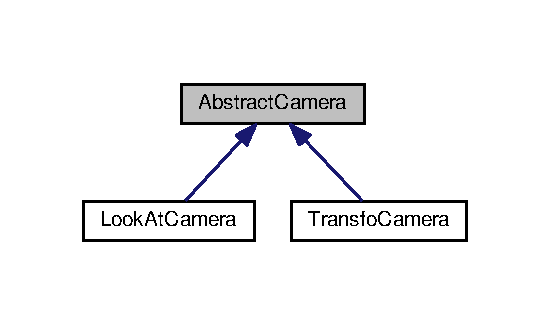
\includegraphics[width=264pt]{class_abstract_camera__inherit__graph}
\end{center}
\end{figure}
\subsection*{Public Types}
\begin{DoxyCompactItemize}
\item 
enum \hyperlink{class_abstract_camera_a4d3cc29d2eb150eada1bb387648eae98}{Type\+Repere} \{ \hyperlink{class_abstract_camera_a4d3cc29d2eb150eada1bb387648eae98a4136744a39efe4b86f6743eecc488eb8}{M\+O\+N\+D\+E} = 0, 
\hyperlink{class_abstract_camera_a4d3cc29d2eb150eada1bb387648eae98a7fc33f57f9cabf6771b5fdfa9c64494c}{C\+A\+M\+E\+R\+A} = 1
 \}
\end{DoxyCompactItemize}
\subsection*{Public Member Functions}
\begin{DoxyCompactItemize}
\item 
\hyperlink{class_abstract_camera_a66df51ce45fb8be484c56161fe326129}{Abstract\+Camera} (double px, double py, double pz, double vx, double vy, double vz, double vertx, double verty, double vertz, double zproche=1, double zeloigne=500, double angle\+Ouverture=50)
\item 
virtual \hyperlink{class_abstract_camera_addf550f9f41d04bd6651b19d795bdabe}{$\sim$\+Abstract\+Camera} ()
\item 
void \hyperlink{class_abstract_camera_a7231574aecbb95374f3b6f82349608a4}{Redimensionnement} (int w, int h)
\begin{DoxyCompactList}\small\item\em Redimensionnement de la fenêtre. \end{DoxyCompactList}\item 
void \hyperlink{class_abstract_camera_a14ae54182b566740e1285ad33dfc6b2b}{Changement\+Angle} (double angle\+Ouverture\+Y)
\begin{DoxyCompactList}\small\item\em Changement de l'angle d'ouverture. \end{DoxyCompactList}\item 
void \hyperlink{class_abstract_camera_a2685cf0a29e7dac3ca7c8b6d6b545810}{Apply\+Perspective\+Projection} (double angle\+Ouverture\+Y, double aspect, double z\+Proche, double z\+Eloigne)
\begin{DoxyCompactList}\small\item\em Application de la projection. \end{DoxyCompactList}\item 
virtual void \hyperlink{class_abstract_camera_aeaa6522c54a923a50137d2c0ca54238b}{Changer\+Repere\+Camera} (double position\mbox{[}3\mbox{]}, double point\+De\+Visee\mbox{[}3\mbox{]}, double vecteur\+Vertical\mbox{[}3\mbox{]})=0
\begin{DoxyCompactList}\small\item\em Changement du repère de la caméra. \end{DoxyCompactList}\item 
virtual void \hyperlink{class_abstract_camera_a4bfcc6ed8980d64cf1d43d7dcb60129b}{Changer\+Repere\+Camera} ()=0
\begin{DoxyCompactList}\small\item\em Changement du repère de la caméra. \end{DoxyCompactList}\item 
void \hyperlink{class_abstract_camera_a658752e59c42aacadb3e05b811c5b733}{Zoumage} (bool forward)
\begin{DoxyCompactList}\small\item\em Zoom de la caméra. \end{DoxyCompactList}\item 
void \hyperlink{class_abstract_camera_abce3fc447411ab866d33c80e3a787425}{Set\+Postion} (double px, double py, double pz)
\begin{DoxyCompactList}\small\item\em Setter de la position. \end{DoxyCompactList}\item 
void \hyperlink{class_abstract_camera_a6d987b85b99a72dc2dbae2bad3add3c2}{Set\+Visee} (double vx, double vy, double vz)
\begin{DoxyCompactList}\small\item\em Setter de la visée. \end{DoxyCompactList}\item 
void \hyperlink{class_abstract_camera_a18b29aed678919cf853368d6708dd218}{Set\+Vertical} (double vertx, double verty, double vertz)
\begin{DoxyCompactList}\small\item\em Setter de la verticale. \end{DoxyCompactList}\item 
void \hyperlink{class_abstract_camera_a2cc297f1c766623fc890030ce343a145}{Set\+Angle\+Ouverture} (double a)
\begin{DoxyCompactList}\small\item\em Setter de l'angle d'ouverture. \end{DoxyCompactList}\item 
double $\ast$ \hyperlink{class_abstract_camera_a59cd96f58f9bf36a8835f28c4b83f71d}{Get\+Position} ()
\begin{DoxyCompactList}\small\item\em Getter de la position. \end{DoxyCompactList}\item 
double $\ast$ \hyperlink{class_abstract_camera_ae78023d4ab2a0b5f09c9704d0358351e}{Get\+Visee} ()
\begin{DoxyCompactList}\small\item\em Getter de la visée. \end{DoxyCompactList}\item 
double $\ast$ \hyperlink{class_abstract_camera_a26576ea56602025af025c67b63c1a081}{Get\+Vertical} ()
\begin{DoxyCompactList}\small\item\em Getter de la verticale. \end{DoxyCompactList}\item 
double \hyperlink{class_abstract_camera_ada5eaaeda93679236af0700e932eccd6}{Get\+Angle\+Ouverture} () const 
\begin{DoxyCompactList}\small\item\em Getter de l'angle d'ouverture. \end{DoxyCompactList}\end{DoxyCompactItemize}
\subsection*{Protected Attributes}
\begin{DoxyCompactItemize}
\item 
double \hyperlink{class_abstract_camera_aacd5e7f2d881e719f254a1d6e2904b91}{m\+Position} \mbox{[}3\mbox{]}
\begin{DoxyCompactList}\small\item\em Position de la caméra. \end{DoxyCompactList}\item 
double \hyperlink{class_abstract_camera_a5c7db642de2add50fad69539a8b220d8}{m\+Visee} \mbox{[}3\mbox{]}
\begin{DoxyCompactList}\small\item\em Point de visée de la caméra. \end{DoxyCompactList}\item 
double \hyperlink{class_abstract_camera_a64675d12169d6383a9371d7fd710a441}{m\+Vertical} \mbox{[}3\mbox{]}
\begin{DoxyCompactList}\small\item\em Vecteur vertical de la caméra. \end{DoxyCompactList}\item 
double \hyperlink{class_abstract_camera_a408e219c2aed42b6aa4f9198c252d10a}{m\+Z\+\_\+proche}
\begin{DoxyCompactList}\small\item\em Distance du plan proche. \end{DoxyCompactList}\item 
double \hyperlink{class_abstract_camera_a8e076553a55c8e2f19948bdf4ea01be1}{m\+Z\+\_\+eloigne}
\begin{DoxyCompactList}\small\item\em Distance du plan éloigné \end{DoxyCompactList}\item 
double \hyperlink{class_abstract_camera_a5facdc9b6a67be951f8adea9d7ed8756}{m\+Angle\+Ouverture}
\begin{DoxyCompactList}\small\item\em Angle d'ouverture de la caméra. \end{DoxyCompactList}\item 
double \hyperlink{class_abstract_camera_a84ea352c679449eeef49d92274bfc9e0}{m\+Aspect}
\begin{DoxyCompactList}\small\item\em Aspect de la caméra. \end{DoxyCompactList}\end{DoxyCompactItemize}


\subsection{Detailed Description}
Classe de caméra abstraite Classe de caméra abstraite. 

\subsection{Member Enumeration Documentation}
\hypertarget{class_abstract_camera_a4d3cc29d2eb150eada1bb387648eae98}{\index{Abstract\+Camera@{Abstract\+Camera}!Type\+Repere@{Type\+Repere}}
\index{Type\+Repere@{Type\+Repere}!Abstract\+Camera@{Abstract\+Camera}}
\subsubsection[{Type\+Repere}]{\setlength{\rightskip}{0pt plus 5cm}enum {\bf Abstract\+Camera\+::\+Type\+Repere}}}\label{class_abstract_camera_a4d3cc29d2eb150eada1bb387648eae98}
Types de repères supportés ( repères du monde et de l a camé ra ) \begin{Desc}
\item[Enumerator]\par
\begin{description}
\index{M\+O\+N\+D\+E@{M\+O\+N\+D\+E}!Abstract\+Camera@{Abstract\+Camera}}\index{Abstract\+Camera@{Abstract\+Camera}!M\+O\+N\+D\+E@{M\+O\+N\+D\+E}}\item[{\em 
\hypertarget{class_abstract_camera_a4d3cc29d2eb150eada1bb387648eae98a4136744a39efe4b86f6743eecc488eb8}{M\+O\+N\+D\+E}\label{class_abstract_camera_a4d3cc29d2eb150eada1bb387648eae98a4136744a39efe4b86f6743eecc488eb8}
}]\index{C\+A\+M\+E\+R\+A@{C\+A\+M\+E\+R\+A}!Abstract\+Camera@{Abstract\+Camera}}\index{Abstract\+Camera@{Abstract\+Camera}!C\+A\+M\+E\+R\+A@{C\+A\+M\+E\+R\+A}}\item[{\em 
\hypertarget{class_abstract_camera_a4d3cc29d2eb150eada1bb387648eae98a7fc33f57f9cabf6771b5fdfa9c64494c}{C\+A\+M\+E\+R\+A}\label{class_abstract_camera_a4d3cc29d2eb150eada1bb387648eae98a7fc33f57f9cabf6771b5fdfa9c64494c}
}]\end{description}
\end{Desc}


\subsection{Constructor \& Destructor Documentation}
\hypertarget{class_abstract_camera_a66df51ce45fb8be484c56161fe326129}{\index{Abstract\+Camera@{Abstract\+Camera}!Abstract\+Camera@{Abstract\+Camera}}
\index{Abstract\+Camera@{Abstract\+Camera}!Abstract\+Camera@{Abstract\+Camera}}
\subsubsection[{Abstract\+Camera}]{\setlength{\rightskip}{0pt plus 5cm}Abstract\+Camera\+::\+Abstract\+Camera (
\begin{DoxyParamCaption}
\item[{double}]{px, }
\item[{double}]{py, }
\item[{double}]{pz, }
\item[{double}]{vx, }
\item[{double}]{vy, }
\item[{double}]{vz, }
\item[{double}]{vertx, }
\item[{double}]{verty, }
\item[{double}]{vertz, }
\item[{double}]{zproche = {\ttfamily 1}, }
\item[{double}]{zeloigne = {\ttfamily 500}, }
\item[{double}]{angle\+Ouverture = {\ttfamily 50}}
\end{DoxyParamCaption}
)}}\label{class_abstract_camera_a66df51ce45fb8be484c56161fe326129}
Constructeur \hypertarget{class_abstract_camera_addf550f9f41d04bd6651b19d795bdabe}{\index{Abstract\+Camera@{Abstract\+Camera}!````~Abstract\+Camera@{$\sim$\+Abstract\+Camera}}
\index{````~Abstract\+Camera@{$\sim$\+Abstract\+Camera}!Abstract\+Camera@{Abstract\+Camera}}
\subsubsection[{$\sim$\+Abstract\+Camera}]{\setlength{\rightskip}{0pt plus 5cm}Abstract\+Camera\+::$\sim$\+Abstract\+Camera (
\begin{DoxyParamCaption}
{}
\end{DoxyParamCaption}
)\hspace{0.3cm}{\ttfamily [virtual]}}}\label{class_abstract_camera_addf550f9f41d04bd6651b19d795bdabe}
Destructeur 

\subsection{Member Function Documentation}
\hypertarget{class_abstract_camera_a2685cf0a29e7dac3ca7c8b6d6b545810}{\index{Abstract\+Camera@{Abstract\+Camera}!Apply\+Perspective\+Projection@{Apply\+Perspective\+Projection}}
\index{Apply\+Perspective\+Projection@{Apply\+Perspective\+Projection}!Abstract\+Camera@{Abstract\+Camera}}
\subsubsection[{Apply\+Perspective\+Projection}]{\setlength{\rightskip}{0pt plus 5cm}void Abstract\+Camera\+::\+Apply\+Perspective\+Projection (
\begin{DoxyParamCaption}
\item[{double}]{angle\+Ouverture\+Y, }
\item[{double}]{aspect, }
\item[{double}]{z\+Proche, }
\item[{double}]{z\+Eloigne}
\end{DoxyParamCaption}
)}}\label{class_abstract_camera_a2685cf0a29e7dac3ca7c8b6d6b545810}


Application de la projection. 


\begin{DoxyParams}{Parameters}
{\em double} & \\
\hline
{\em double} & \\
\hline
{\em double} & \\
\hline
{\em double} & \\
\hline
\end{DoxyParams}
\begin{DoxyReturn}{Returns}
void 
\end{DoxyReturn}
\hypertarget{class_abstract_camera_a14ae54182b566740e1285ad33dfc6b2b}{\index{Abstract\+Camera@{Abstract\+Camera}!Changement\+Angle@{Changement\+Angle}}
\index{Changement\+Angle@{Changement\+Angle}!Abstract\+Camera@{Abstract\+Camera}}
\subsubsection[{Changement\+Angle}]{\setlength{\rightskip}{0pt plus 5cm}void Abstract\+Camera\+::\+Changement\+Angle (
\begin{DoxyParamCaption}
\item[{double}]{angle\+Ouverture\+Y}
\end{DoxyParamCaption}
)}}\label{class_abstract_camera_a14ae54182b566740e1285ad33dfc6b2b}


Changement de l'angle d'ouverture. 


\begin{DoxyParams}{Parameters}
{\em double} & \+: angle \\
\hline
\end{DoxyParams}
\hypertarget{class_abstract_camera_aeaa6522c54a923a50137d2c0ca54238b}{\index{Abstract\+Camera@{Abstract\+Camera}!Changer\+Repere\+Camera@{Changer\+Repere\+Camera}}
\index{Changer\+Repere\+Camera@{Changer\+Repere\+Camera}!Abstract\+Camera@{Abstract\+Camera}}
\subsubsection[{Changer\+Repere\+Camera}]{\setlength{\rightskip}{0pt plus 5cm}virtual void Abstract\+Camera\+::\+Changer\+Repere\+Camera (
\begin{DoxyParamCaption}
\item[{double}]{position\mbox{[}3\mbox{]}, }
\item[{double}]{point\+De\+Visee\mbox{[}3\mbox{]}, }
\item[{double}]{vecteur\+Vertical\mbox{[}3\mbox{]}}
\end{DoxyParamCaption}
)\hspace{0.3cm}{\ttfamily [pure virtual]}}}\label{class_abstract_camera_aeaa6522c54a923a50137d2c0ca54238b}


Changement du repère de la caméra. 


\begin{DoxyParams}{Parameters}
{\em double\mbox{[}$\,$\mbox{]}} & position de la caméra \\
\hline
{\em double\mbox{[}$\,$\mbox{]}} & point de visée de la caméra \\
\hline
{\em double\mbox{[}$\,$\mbox{]}} & vertical de la caméra \\
\hline
\end{DoxyParams}
\begin{DoxyReturn}{Returns}
void 
\end{DoxyReturn}


Implemented in \hyperlink{class_transfo_camera_af56c28b564652b71b7040084aaec8ff9}{Transfo\+Camera}, and \hyperlink{class_look_at_camera_a0904e7cb4cc17c9d8dd54d8a394eb9cc}{Look\+At\+Camera}.

\hypertarget{class_abstract_camera_a4bfcc6ed8980d64cf1d43d7dcb60129b}{\index{Abstract\+Camera@{Abstract\+Camera}!Changer\+Repere\+Camera@{Changer\+Repere\+Camera}}
\index{Changer\+Repere\+Camera@{Changer\+Repere\+Camera}!Abstract\+Camera@{Abstract\+Camera}}
\subsubsection[{Changer\+Repere\+Camera}]{\setlength{\rightskip}{0pt plus 5cm}virtual void Abstract\+Camera\+::\+Changer\+Repere\+Camera (
\begin{DoxyParamCaption}
{}
\end{DoxyParamCaption}
)\hspace{0.3cm}{\ttfamily [pure virtual]}}}\label{class_abstract_camera_a4bfcc6ed8980d64cf1d43d7dcb60129b}


Changement du repère de la caméra. 

\begin{DoxyReturn}{Returns}
void 
\end{DoxyReturn}


Implemented in \hyperlink{class_transfo_camera_a1d02bd6398256954713d1c239d2ebcba}{Transfo\+Camera}, and \hyperlink{class_look_at_camera_ac8ff2cf45773bf8f27fa9972e1f48c5d}{Look\+At\+Camera}.

\hypertarget{class_abstract_camera_ada5eaaeda93679236af0700e932eccd6}{\index{Abstract\+Camera@{Abstract\+Camera}!Get\+Angle\+Ouverture@{Get\+Angle\+Ouverture}}
\index{Get\+Angle\+Ouverture@{Get\+Angle\+Ouverture}!Abstract\+Camera@{Abstract\+Camera}}
\subsubsection[{Get\+Angle\+Ouverture}]{\setlength{\rightskip}{0pt plus 5cm}double Abstract\+Camera\+::\+Get\+Angle\+Ouverture (
\begin{DoxyParamCaption}
{}
\end{DoxyParamCaption}
) const}}\label{class_abstract_camera_ada5eaaeda93679236af0700e932eccd6}


Getter de l'angle d'ouverture. 


\begin{DoxyParams}{Parameters}
{\em void} & \\
\hline
\end{DoxyParams}
\begin{DoxyReturn}{Returns}
angle d'ouverture 
\end{DoxyReturn}
\hypertarget{class_abstract_camera_a59cd96f58f9bf36a8835f28c4b83f71d}{\index{Abstract\+Camera@{Abstract\+Camera}!Get\+Position@{Get\+Position}}
\index{Get\+Position@{Get\+Position}!Abstract\+Camera@{Abstract\+Camera}}
\subsubsection[{Get\+Position}]{\setlength{\rightskip}{0pt plus 5cm}double $\ast$ Abstract\+Camera\+::\+Get\+Position (
\begin{DoxyParamCaption}
{}
\end{DoxyParamCaption}
)}}\label{class_abstract_camera_a59cd96f58f9bf36a8835f28c4b83f71d}


Getter de la position. 


\begin{DoxyParams}{Parameters}
{\em void} & \\
\hline
\end{DoxyParams}
\begin{DoxyReturn}{Returns}
position 
\end{DoxyReturn}
\hypertarget{class_abstract_camera_a26576ea56602025af025c67b63c1a081}{\index{Abstract\+Camera@{Abstract\+Camera}!Get\+Vertical@{Get\+Vertical}}
\index{Get\+Vertical@{Get\+Vertical}!Abstract\+Camera@{Abstract\+Camera}}
\subsubsection[{Get\+Vertical}]{\setlength{\rightskip}{0pt plus 5cm}double $\ast$ Abstract\+Camera\+::\+Get\+Vertical (
\begin{DoxyParamCaption}
{}
\end{DoxyParamCaption}
)}}\label{class_abstract_camera_a26576ea56602025af025c67b63c1a081}


Getter de la verticale. 


\begin{DoxyParams}{Parameters}
{\em void} & \\
\hline
\end{DoxyParams}
\begin{DoxyReturn}{Returns}
verticale 
\end{DoxyReturn}
\hypertarget{class_abstract_camera_ae78023d4ab2a0b5f09c9704d0358351e}{\index{Abstract\+Camera@{Abstract\+Camera}!Get\+Visee@{Get\+Visee}}
\index{Get\+Visee@{Get\+Visee}!Abstract\+Camera@{Abstract\+Camera}}
\subsubsection[{Get\+Visee}]{\setlength{\rightskip}{0pt plus 5cm}double $\ast$ Abstract\+Camera\+::\+Get\+Visee (
\begin{DoxyParamCaption}
{}
\end{DoxyParamCaption}
)}}\label{class_abstract_camera_ae78023d4ab2a0b5f09c9704d0358351e}


Getter de la visée. 


\begin{DoxyParams}{Parameters}
{\em void} & \\
\hline
\end{DoxyParams}
\begin{DoxyReturn}{Returns}
visée 
\end{DoxyReturn}
\hypertarget{class_abstract_camera_a7231574aecbb95374f3b6f82349608a4}{\index{Abstract\+Camera@{Abstract\+Camera}!Redimensionnement@{Redimensionnement}}
\index{Redimensionnement@{Redimensionnement}!Abstract\+Camera@{Abstract\+Camera}}
\subsubsection[{Redimensionnement}]{\setlength{\rightskip}{0pt plus 5cm}void Abstract\+Camera\+::\+Redimensionnement (
\begin{DoxyParamCaption}
\item[{int}]{w, }
\item[{int}]{h}
\end{DoxyParamCaption}
)}}\label{class_abstract_camera_a7231574aecbb95374f3b6f82349608a4}


Redimensionnement de la fenêtre. 


\begin{DoxyParams}{Parameters}
{\em Largeur} & de la fenêtre \\
\hline
{\em Hauteur} & de la fenêtre \\
\hline
\end{DoxyParams}
\hypertarget{class_abstract_camera_a2cc297f1c766623fc890030ce343a145}{\index{Abstract\+Camera@{Abstract\+Camera}!Set\+Angle\+Ouverture@{Set\+Angle\+Ouverture}}
\index{Set\+Angle\+Ouverture@{Set\+Angle\+Ouverture}!Abstract\+Camera@{Abstract\+Camera}}
\subsubsection[{Set\+Angle\+Ouverture}]{\setlength{\rightskip}{0pt plus 5cm}void Abstract\+Camera\+::\+Set\+Angle\+Ouverture (
\begin{DoxyParamCaption}
\item[{double}]{a}
\end{DoxyParamCaption}
)}}\label{class_abstract_camera_a2cc297f1c766623fc890030ce343a145}


Setter de l'angle d'ouverture. 


\begin{DoxyParams}{Parameters}
{\em Nouvel} & angle \\
\hline
\end{DoxyParams}
\begin{DoxyReturn}{Returns}
void 
\end{DoxyReturn}
\hypertarget{class_abstract_camera_abce3fc447411ab866d33c80e3a787425}{\index{Abstract\+Camera@{Abstract\+Camera}!Set\+Postion@{Set\+Postion}}
\index{Set\+Postion@{Set\+Postion}!Abstract\+Camera@{Abstract\+Camera}}
\subsubsection[{Set\+Postion}]{\setlength{\rightskip}{0pt plus 5cm}void Abstract\+Camera\+::\+Set\+Postion (
\begin{DoxyParamCaption}
\item[{double}]{px, }
\item[{double}]{py, }
\item[{double}]{pz}
\end{DoxyParamCaption}
)}}\label{class_abstract_camera_abce3fc447411ab866d33c80e3a787425}


Setter de la position. 


\begin{DoxyParams}{Parameters}
{\em Nouvelle} & position \\
\hline
\end{DoxyParams}
\begin{DoxyReturn}{Returns}
void 
\end{DoxyReturn}
\hypertarget{class_abstract_camera_a18b29aed678919cf853368d6708dd218}{\index{Abstract\+Camera@{Abstract\+Camera}!Set\+Vertical@{Set\+Vertical}}
\index{Set\+Vertical@{Set\+Vertical}!Abstract\+Camera@{Abstract\+Camera}}
\subsubsection[{Set\+Vertical}]{\setlength{\rightskip}{0pt plus 5cm}void Abstract\+Camera\+::\+Set\+Vertical (
\begin{DoxyParamCaption}
\item[{double}]{vertx, }
\item[{double}]{verty, }
\item[{double}]{vertz}
\end{DoxyParamCaption}
)}}\label{class_abstract_camera_a18b29aed678919cf853368d6708dd218}


Setter de la verticale. 


\begin{DoxyParams}{Parameters}
{\em Nouvelle} & position \\
\hline
\end{DoxyParams}
\begin{DoxyReturn}{Returns}
void 
\end{DoxyReturn}
\hypertarget{class_abstract_camera_a6d987b85b99a72dc2dbae2bad3add3c2}{\index{Abstract\+Camera@{Abstract\+Camera}!Set\+Visee@{Set\+Visee}}
\index{Set\+Visee@{Set\+Visee}!Abstract\+Camera@{Abstract\+Camera}}
\subsubsection[{Set\+Visee}]{\setlength{\rightskip}{0pt plus 5cm}void Abstract\+Camera\+::\+Set\+Visee (
\begin{DoxyParamCaption}
\item[{double}]{vx, }
\item[{double}]{vy, }
\item[{double}]{vz}
\end{DoxyParamCaption}
)}}\label{class_abstract_camera_a6d987b85b99a72dc2dbae2bad3add3c2}


Setter de la visée. 


\begin{DoxyParams}{Parameters}
{\em Nouvelle} & position \\
\hline
\end{DoxyParams}
\begin{DoxyReturn}{Returns}
void 
\end{DoxyReturn}
\hypertarget{class_abstract_camera_a658752e59c42aacadb3e05b811c5b733}{\index{Abstract\+Camera@{Abstract\+Camera}!Zoumage@{Zoumage}}
\index{Zoumage@{Zoumage}!Abstract\+Camera@{Abstract\+Camera}}
\subsubsection[{Zoumage}]{\setlength{\rightskip}{0pt plus 5cm}void Abstract\+Camera\+::\+Zoumage (
\begin{DoxyParamCaption}
\item[{bool}]{forward}
\end{DoxyParamCaption}
)}}\label{class_abstract_camera_a658752e59c42aacadb3e05b811c5b733}


Zoom de la caméra. 


\begin{DoxyParams}{Parameters}
{\em true} & \+: avancer \\
\hline
\end{DoxyParams}
\begin{DoxyReturn}{Returns}
void 
\end{DoxyReturn}


\subsection{Member Data Documentation}
\hypertarget{class_abstract_camera_a5facdc9b6a67be951f8adea9d7ed8756}{\index{Abstract\+Camera@{Abstract\+Camera}!m\+Angle\+Ouverture@{m\+Angle\+Ouverture}}
\index{m\+Angle\+Ouverture@{m\+Angle\+Ouverture}!Abstract\+Camera@{Abstract\+Camera}}
\subsubsection[{m\+Angle\+Ouverture}]{\setlength{\rightskip}{0pt plus 5cm}double Abstract\+Camera\+::m\+Angle\+Ouverture\hspace{0.3cm}{\ttfamily [protected]}}}\label{class_abstract_camera_a5facdc9b6a67be951f8adea9d7ed8756}


Angle d'ouverture de la caméra. 

\hypertarget{class_abstract_camera_a84ea352c679449eeef49d92274bfc9e0}{\index{Abstract\+Camera@{Abstract\+Camera}!m\+Aspect@{m\+Aspect}}
\index{m\+Aspect@{m\+Aspect}!Abstract\+Camera@{Abstract\+Camera}}
\subsubsection[{m\+Aspect}]{\setlength{\rightskip}{0pt plus 5cm}double Abstract\+Camera\+::m\+Aspect\hspace{0.3cm}{\ttfamily [protected]}}}\label{class_abstract_camera_a84ea352c679449eeef49d92274bfc9e0}


Aspect de la caméra. 

\hypertarget{class_abstract_camera_aacd5e7f2d881e719f254a1d6e2904b91}{\index{Abstract\+Camera@{Abstract\+Camera}!m\+Position@{m\+Position}}
\index{m\+Position@{m\+Position}!Abstract\+Camera@{Abstract\+Camera}}
\subsubsection[{m\+Position}]{\setlength{\rightskip}{0pt plus 5cm}double Abstract\+Camera\+::m\+Position\mbox{[}3\mbox{]}\hspace{0.3cm}{\ttfamily [protected]}}}\label{class_abstract_camera_aacd5e7f2d881e719f254a1d6e2904b91}


Position de la caméra. 

\hypertarget{class_abstract_camera_a64675d12169d6383a9371d7fd710a441}{\index{Abstract\+Camera@{Abstract\+Camera}!m\+Vertical@{m\+Vertical}}
\index{m\+Vertical@{m\+Vertical}!Abstract\+Camera@{Abstract\+Camera}}
\subsubsection[{m\+Vertical}]{\setlength{\rightskip}{0pt plus 5cm}double Abstract\+Camera\+::m\+Vertical\mbox{[}3\mbox{]}\hspace{0.3cm}{\ttfamily [protected]}}}\label{class_abstract_camera_a64675d12169d6383a9371d7fd710a441}


Vecteur vertical de la caméra. 

\hypertarget{class_abstract_camera_a5c7db642de2add50fad69539a8b220d8}{\index{Abstract\+Camera@{Abstract\+Camera}!m\+Visee@{m\+Visee}}
\index{m\+Visee@{m\+Visee}!Abstract\+Camera@{Abstract\+Camera}}
\subsubsection[{m\+Visee}]{\setlength{\rightskip}{0pt plus 5cm}double Abstract\+Camera\+::m\+Visee\mbox{[}3\mbox{]}\hspace{0.3cm}{\ttfamily [protected]}}}\label{class_abstract_camera_a5c7db642de2add50fad69539a8b220d8}


Point de visée de la caméra. 

\hypertarget{class_abstract_camera_a8e076553a55c8e2f19948bdf4ea01be1}{\index{Abstract\+Camera@{Abstract\+Camera}!m\+Z\+\_\+eloigne@{m\+Z\+\_\+eloigne}}
\index{m\+Z\+\_\+eloigne@{m\+Z\+\_\+eloigne}!Abstract\+Camera@{Abstract\+Camera}}
\subsubsection[{m\+Z\+\_\+eloigne}]{\setlength{\rightskip}{0pt plus 5cm}double Abstract\+Camera\+::m\+Z\+\_\+eloigne\hspace{0.3cm}{\ttfamily [protected]}}}\label{class_abstract_camera_a8e076553a55c8e2f19948bdf4ea01be1}


Distance du plan éloigné 

\hypertarget{class_abstract_camera_a408e219c2aed42b6aa4f9198c252d10a}{\index{Abstract\+Camera@{Abstract\+Camera}!m\+Z\+\_\+proche@{m\+Z\+\_\+proche}}
\index{m\+Z\+\_\+proche@{m\+Z\+\_\+proche}!Abstract\+Camera@{Abstract\+Camera}}
\subsubsection[{m\+Z\+\_\+proche}]{\setlength{\rightskip}{0pt plus 5cm}double Abstract\+Camera\+::m\+Z\+\_\+proche\hspace{0.3cm}{\ttfamily [protected]}}}\label{class_abstract_camera_a408e219c2aed42b6aa4f9198c252d10a}


Distance du plan proche. 



The documentation for this class was generated from the following files\+:\begin{DoxyCompactItemize}
\item 
src/\hyperlink{abstract_camera_8hpp}{abstract\+Camera.\+hpp}\item 
src/\hyperlink{abstract_camera_8cpp}{abstract\+Camera.\+cpp}\end{DoxyCompactItemize}

\hypertarget{class_abstract_scene}{\section{Abstract\+Scene Class Reference}
\label{class_abstract_scene}\index{Abstract\+Scene@{Abstract\+Scene}}
}


{\ttfamily \#include $<$abstract\+Scene.\+hpp$>$}



Inheritance diagram for Abstract\+Scene\+:
\nopagebreak
\begin{figure}[H]
\begin{center}
\leavevmode
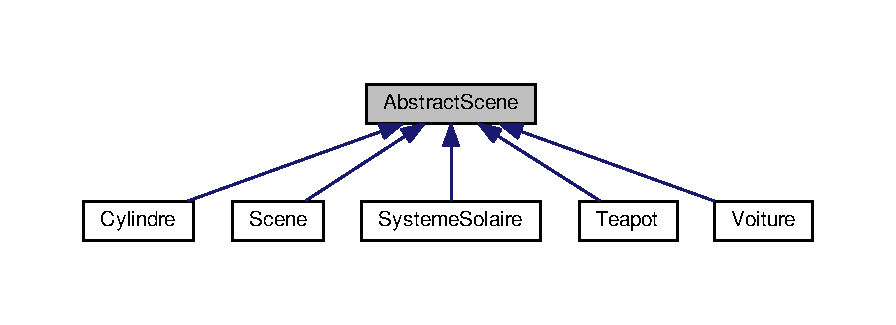
\includegraphics[width=350pt]{class_abstract_scene__inherit__graph}
\end{center}
\end{figure}


Collaboration diagram for Abstract\+Scene\+:
\nopagebreak
\begin{figure}[H]
\begin{center}
\leavevmode
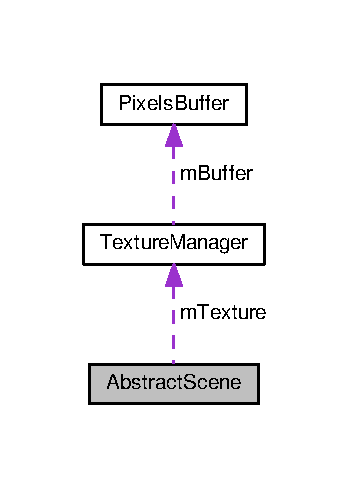
\includegraphics[width=169pt]{class_abstract_scene__coll__graph}
\end{center}
\end{figure}
\subsection*{Public Member Functions}
\begin{DoxyCompactItemize}
\item 
virtual \hyperlink{class_abstract_scene_a82b4811120763f71a5e81a9d72b339f3}{$\sim$\+Abstract\+Scene} ()
\item 
virtual void \hyperlink{class_abstract_scene_aaf2f4c7aa4a6401f66bed00a51d8e64f}{render} ()
\begin{DoxyCompactList}\small\item\em Affiche la scene courante. \end{DoxyCompactList}\end{DoxyCompactItemize}
\subsection*{Protected Member Functions}
\begin{DoxyCompactItemize}
\item 
\hyperlink{class_abstract_scene_ae4b1176cfbb35e9ffc3b7021d3274cc4}{Abstract\+Scene} ()
\item 
\hyperlink{class_abstract_scene_a6f42922b5dc67eb56aeb2246c39c02ae}{Abstract\+Scene} (const char $\ast$path)
\end{DoxyCompactItemize}
\subsection*{Protected Attributes}
\begin{DoxyCompactItemize}
\item 
\hyperlink{struct_texture_manager}{Texture\+Manager} \hyperlink{class_abstract_scene_af5c8041d61ff5700c02e365345c06f67}{m\+Texture}
\end{DoxyCompactItemize}


\subsection{Detailed Description}
Classe mere des types de scenes disponibles 

\subsection{Constructor \& Destructor Documentation}
\hypertarget{class_abstract_scene_ae4b1176cfbb35e9ffc3b7021d3274cc4}{\index{Abstract\+Scene@{Abstract\+Scene}!Abstract\+Scene@{Abstract\+Scene}}
\index{Abstract\+Scene@{Abstract\+Scene}!Abstract\+Scene@{Abstract\+Scene}}
\subsubsection[{Abstract\+Scene}]{\setlength{\rightskip}{0pt plus 5cm}Abstract\+Scene\+::\+Abstract\+Scene (
\begin{DoxyParamCaption}
{}
\end{DoxyParamCaption}
)\hspace{0.3cm}{\ttfamily [inline]}, {\ttfamily [protected]}}}\label{class_abstract_scene_ae4b1176cfbb35e9ffc3b7021d3274cc4}
\hypertarget{class_abstract_scene_a6f42922b5dc67eb56aeb2246c39c02ae}{\index{Abstract\+Scene@{Abstract\+Scene}!Abstract\+Scene@{Abstract\+Scene}}
\index{Abstract\+Scene@{Abstract\+Scene}!Abstract\+Scene@{Abstract\+Scene}}
\subsubsection[{Abstract\+Scene}]{\setlength{\rightskip}{0pt plus 5cm}Abstract\+Scene\+::\+Abstract\+Scene (
\begin{DoxyParamCaption}
\item[{const char $\ast$}]{path}
\end{DoxyParamCaption}
)\hspace{0.3cm}{\ttfamily [inline]}, {\ttfamily [protected]}}}\label{class_abstract_scene_a6f42922b5dc67eb56aeb2246c39c02ae}
\hypertarget{class_abstract_scene_a82b4811120763f71a5e81a9d72b339f3}{\index{Abstract\+Scene@{Abstract\+Scene}!````~Abstract\+Scene@{$\sim$\+Abstract\+Scene}}
\index{````~Abstract\+Scene@{$\sim$\+Abstract\+Scene}!Abstract\+Scene@{Abstract\+Scene}}
\subsubsection[{$\sim$\+Abstract\+Scene}]{\setlength{\rightskip}{0pt plus 5cm}virtual Abstract\+Scene\+::$\sim$\+Abstract\+Scene (
\begin{DoxyParamCaption}
{}
\end{DoxyParamCaption}
)\hspace{0.3cm}{\ttfamily [inline]}, {\ttfamily [virtual]}}}\label{class_abstract_scene_a82b4811120763f71a5e81a9d72b339f3}


\subsection{Member Function Documentation}
\hypertarget{class_abstract_scene_aaf2f4c7aa4a6401f66bed00a51d8e64f}{\index{Abstract\+Scene@{Abstract\+Scene}!render@{render}}
\index{render@{render}!Abstract\+Scene@{Abstract\+Scene}}
\subsubsection[{render}]{\setlength{\rightskip}{0pt plus 5cm}virtual void Abstract\+Scene\+::render (
\begin{DoxyParamCaption}
{}
\end{DoxyParamCaption}
)\hspace{0.3cm}{\ttfamily [inline]}, {\ttfamily [virtual]}}}\label{class_abstract_scene_aaf2f4c7aa4a6401f66bed00a51d8e64f}


Affiche la scene courante. 



Reimplemented in \hyperlink{class_cylindre_a1dfb851bf7fa789abb927361814ad1fe}{Cylindre}, \hyperlink{class_voiture_a4abe5b41fc48c9cbdd0da7780dcd9a53}{Voiture}, \hyperlink{class_scene_a4ddf2d16f371ee9533b3faf1dd5ddfb1}{Scene}, \hyperlink{class_systeme_solaire_a500de47c923d4284867416bc007b9c11}{Systeme\+Solaire}, and \hyperlink{class_teapot_aababf7bd2833ebd3c34564b45b902163}{Teapot}.



\subsection{Member Data Documentation}
\hypertarget{class_abstract_scene_af5c8041d61ff5700c02e365345c06f67}{\index{Abstract\+Scene@{Abstract\+Scene}!m\+Texture@{m\+Texture}}
\index{m\+Texture@{m\+Texture}!Abstract\+Scene@{Abstract\+Scene}}
\subsubsection[{m\+Texture}]{\setlength{\rightskip}{0pt plus 5cm}{\bf Texture\+Manager} Abstract\+Scene\+::m\+Texture\hspace{0.3cm}{\ttfamily [protected]}}}\label{class_abstract_scene_af5c8041d61ff5700c02e365345c06f67}


The documentation for this class was generated from the following file\+:\begin{DoxyCompactItemize}
\item 
src/\hyperlink{abstract_scene_8hpp}{abstract\+Scene.\+hpp}\end{DoxyCompactItemize}

\hypertarget{class_display_manager}{}\section{Display\+Manager Class Reference}
\label{class_display_manager}\index{Display\+Manager@{Display\+Manager}}


Classe de gestion de l\textquotesingle{}affichage. Classe de gestion de l\textquotesingle{}affichage.  




{\ttfamily \#include $<$vue.\+hpp$>$}



Collaboration diagram for Display\+Manager\+:
% FIG 0
\subsection*{Public Member Functions}
\begin{DoxyCompactItemize}
\item 
\hyperlink{class_display_manager_abf11523503126b8ee8ed26d79aba9974}{Display\+Manager} (G\+Lint largeur\+Fenetre, G\+Lint hauteur\+Fenetre)
\begin{DoxyCompactList}\small\item\em Constructeur prenant la géométrie de la fenêtre Initialise les données nécessaires à l\textquotesingle{}affichage. \end{DoxyCompactList}\item 
void \hyperlink{class_display_manager_a692eb24cc56a7ab15ab1fd5a88646a34}{Affichage} ()
\item 
void \hyperlink{class_display_manager_a5372587f56171ad81ac7c0ef686c61f4}{Redimensionnement} (G\+Lint l, G\+Lint h)
\end{DoxyCompactItemize}
\subsection*{Public Attributes}
\begin{DoxyCompactItemize}
\item 
G\+Lint \hyperlink{class_display_manager_a7078a2a1023ebe660ce2e3007a988a62}{m\+Largeur\+Fenetre}
\item 
G\+Lint \hyperlink{class_display_manager_a73b96e4ef8a0621077bcc83bc1dba2cf}{m\+Hauteur\+Fenetre}
\item 
\hyperlink{class_modele}{Modele} \hyperlink{class_display_manager_a0c8ba3fe8aece87fc924847fc8958398}{m\+Modele}
\item 
\hyperlink{class_look_at_camera}{Look\+At\+Camera} \hyperlink{class_display_manager_a17dd81e3974b51416a35c7e9d9232a60}{m\+Camera}
\item 
\hyperlink{struct_light_source_data}{Light\+Source\+Data} \hyperlink{class_display_manager_a012e14f7761f19a3d049aae93f5d694b}{m\+Light}
\end{DoxyCompactItemize}


\subsection{Detailed Description}
Classe de gestion de l\textquotesingle{}affichage. Classe de gestion de l\textquotesingle{}affichage. 

\subsection{Constructor \& Destructor Documentation}
\index{Display\+Manager@{Display\+Manager}!Display\+Manager@{Display\+Manager}}
\index{Display\+Manager@{Display\+Manager}!Display\+Manager@{Display\+Manager}}
\subsubsection[{\texorpdfstring{Display\+Manager(\+G\+Lint largeur\+Fenetre, G\+Lint hauteur\+Fenetre)}{DisplayManager(GLint largeurFenetre, GLint hauteurFenetre)}}]{\setlength{\rightskip}{0pt plus 5cm}Display\+Manager\+::\+Display\+Manager (
\begin{DoxyParamCaption}
\item[{G\+Lint}]{largeur\+Fenetre, }
\item[{G\+Lint}]{hauteur\+Fenetre}
\end{DoxyParamCaption}
)}\hypertarget{class_display_manager_abf11523503126b8ee8ed26d79aba9974}{}\label{class_display_manager_abf11523503126b8ee8ed26d79aba9974}


Constructeur prenant la géométrie de la fenêtre Initialise les données nécessaires à l\textquotesingle{}affichage. 



\subsection{Member Function Documentation}
\index{Display\+Manager@{Display\+Manager}!Affichage@{Affichage}}
\index{Affichage@{Affichage}!Display\+Manager@{Display\+Manager}}
\subsubsection[{\texorpdfstring{Affichage()}{Affichage()}}]{\setlength{\rightskip}{0pt plus 5cm}void Display\+Manager\+::\+Affichage (
\begin{DoxyParamCaption}
{}
\end{DoxyParamCaption}
)}\hypertarget{class_display_manager_a692eb24cc56a7ab15ab1fd5a88646a34}{}\label{class_display_manager_a692eb24cc56a7ab15ab1fd5a88646a34}
Méthode d\textquotesingle{}affichage \index{Display\+Manager@{Display\+Manager}!Redimensionnement@{Redimensionnement}}
\index{Redimensionnement@{Redimensionnement}!Display\+Manager@{Display\+Manager}}
\subsubsection[{\texorpdfstring{Redimensionnement(\+G\+Lint l, G\+Lint h)}{Redimensionnement(GLint l, GLint h)}}]{\setlength{\rightskip}{0pt plus 5cm}void Display\+Manager\+::\+Redimensionnement (
\begin{DoxyParamCaption}
\item[{G\+Lint}]{l, }
\item[{G\+Lint}]{h}
\end{DoxyParamCaption}
)}\hypertarget{class_display_manager_a5372587f56171ad81ac7c0ef686c61f4}{}\label{class_display_manager_a5372587f56171ad81ac7c0ef686c61f4}
Réglage du cadrage pour la vue Doit être rappelée si la taille de la vue change (S\+D\+L\+\_\+\+W\+I\+N\+D\+O\+W\+E\+V\+E\+NT) 
\begin{DoxyParams}{Parameters}
{\em l} & largeur de la (nouvelle) vue \\
\hline
{\em h} & hauteur de la (nouvelle) vue \\
\hline
\end{DoxyParams}


\subsection{Member Data Documentation}
\index{Display\+Manager@{Display\+Manager}!m\+Camera@{m\+Camera}}
\index{m\+Camera@{m\+Camera}!Display\+Manager@{Display\+Manager}}
\subsubsection[{\texorpdfstring{m\+Camera}{mCamera}}]{\setlength{\rightskip}{0pt plus 5cm}{\bf Look\+At\+Camera} Display\+Manager\+::m\+Camera}\hypertarget{class_display_manager_a17dd81e3974b51416a35c7e9d9232a60}{}\label{class_display_manager_a17dd81e3974b51416a35c7e9d9232a60}
\index{Display\+Manager@{Display\+Manager}!m\+Hauteur\+Fenetre@{m\+Hauteur\+Fenetre}}
\index{m\+Hauteur\+Fenetre@{m\+Hauteur\+Fenetre}!Display\+Manager@{Display\+Manager}}
\subsubsection[{\texorpdfstring{m\+Hauteur\+Fenetre}{mHauteurFenetre}}]{\setlength{\rightskip}{0pt plus 5cm}G\+Lint Display\+Manager\+::m\+Hauteur\+Fenetre}\hypertarget{class_display_manager_a73b96e4ef8a0621077bcc83bc1dba2cf}{}\label{class_display_manager_a73b96e4ef8a0621077bcc83bc1dba2cf}
\index{Display\+Manager@{Display\+Manager}!m\+Largeur\+Fenetre@{m\+Largeur\+Fenetre}}
\index{m\+Largeur\+Fenetre@{m\+Largeur\+Fenetre}!Display\+Manager@{Display\+Manager}}
\subsubsection[{\texorpdfstring{m\+Largeur\+Fenetre}{mLargeurFenetre}}]{\setlength{\rightskip}{0pt plus 5cm}G\+Lint Display\+Manager\+::m\+Largeur\+Fenetre}\hypertarget{class_display_manager_a7078a2a1023ebe660ce2e3007a988a62}{}\label{class_display_manager_a7078a2a1023ebe660ce2e3007a988a62}
\index{Display\+Manager@{Display\+Manager}!m\+Light@{m\+Light}}
\index{m\+Light@{m\+Light}!Display\+Manager@{Display\+Manager}}
\subsubsection[{\texorpdfstring{m\+Light}{mLight}}]{\setlength{\rightskip}{0pt plus 5cm}{\bf Light\+Source\+Data} Display\+Manager\+::m\+Light}\hypertarget{class_display_manager_a012e14f7761f19a3d049aae93f5d694b}{}\label{class_display_manager_a012e14f7761f19a3d049aae93f5d694b}
\index{Display\+Manager@{Display\+Manager}!m\+Modele@{m\+Modele}}
\index{m\+Modele@{m\+Modele}!Display\+Manager@{Display\+Manager}}
\subsubsection[{\texorpdfstring{m\+Modele}{mModele}}]{\setlength{\rightskip}{0pt plus 5cm}{\bf Modele} Display\+Manager\+::m\+Modele}\hypertarget{class_display_manager_a0c8ba3fe8aece87fc924847fc8958398}{}\label{class_display_manager_a0c8ba3fe8aece87fc924847fc8958398}


The documentation for this class was generated from the following files\+:\begin{DoxyCompactItemize}
\item 
src/\hyperlink{vue_8hpp}{vue.\+hpp}\item 
src/\hyperlink{vue_8cpp}{vue.\+cpp}\end{DoxyCompactItemize}

\hypertarget{struct_wrapper_s_d_l_1_1_event_controller}{}\section{Wrapper\+S\+DL\+:\+:Event\+Controller Struct Reference}
\label{struct_wrapper_s_d_l_1_1_event_controller}\index{Wrapper\+S\+D\+L\+::\+Event\+Controller@{Wrapper\+S\+D\+L\+::\+Event\+Controller}}


{\ttfamily \#include $<$gui.\+hpp$>$}

\subsection*{Static Public Member Functions}
\begin{DoxyCompactItemize}
\item 
static void \hyperlink{struct_wrapper_s_d_l_1_1_event_controller_a1d120644a13d32238f3372b601a67f80}{Init} (\hyperlink{class_display_manager}{Display\+Manager} $\ast$p\+\_\+\+Params\+Affichage)
\item 
static void \hyperlink{struct_wrapper_s_d_l_1_1_event_controller_a04b13cf306ca88f74c92efb91f4586a3}{Do\+Events\+Loop} (S\+D\+L\+\_\+\+Window $\ast$window, \hyperlink{class_display_manager}{Display\+Manager} $\ast$p\+\_\+\+Params\+Affichage)
\item 
static bool \hyperlink{struct_wrapper_s_d_l_1_1_event_controller_a07cffdf5cf9e8ed68e645239602819d4}{Handle\+\_\+\+S\+D\+L\+\_\+\+Event} (S\+D\+L\+\_\+\+Event $\ast$p\+\_\+evenement, S\+D\+L\+\_\+\+Window $\ast$window, \hyperlink{class_display_manager}{Display\+Manager} $\ast$p\+\_\+\+Params\+Affichage)
\begin{DoxyCompactList}\small\item\em Gestion d\textquotesingle{}un événement S\+DL extrait de la file. \end{DoxyCompactList}\item 
static Uint32 \hyperlink{struct_wrapper_s_d_l_1_1_event_controller_ad4516dc1813e1ab583659ae8386b84af}{Create\+Timer\+Refresh\+Frame} (Uint32 interval, void $\ast$p\+\_\+\+Display\+Manager)
\begin{DoxyCompactList}\small\item\em Callback du timer de raffraichissement de la vue. \end{DoxyCompactList}\end{DoxyCompactItemize}
\subsection*{Static Public Attributes}
\begin{DoxyCompactItemize}
\item 
static S\+D\+L\+\_\+\+Timer\+ID \hyperlink{struct_wrapper_s_d_l_1_1_event_controller_a9d7e9e2326802d622fc1bd9e5a22677b}{m\+Timer\+Id}
\end{DoxyCompactItemize}


\subsection{Detailed Description}
Classe Controleur d\textquotesingle{}événements 

\subsection{Member Function Documentation}
\index{Wrapper\+S\+D\+L\+::\+Event\+Controller@{Wrapper\+S\+D\+L\+::\+Event\+Controller}!Create\+Timer\+Refresh\+Frame@{Create\+Timer\+Refresh\+Frame}}
\index{Create\+Timer\+Refresh\+Frame@{Create\+Timer\+Refresh\+Frame}!Wrapper\+S\+D\+L\+::\+Event\+Controller@{Wrapper\+S\+D\+L\+::\+Event\+Controller}}
\subsubsection[{\texorpdfstring{Create\+Timer\+Refresh\+Frame(\+Uint32 interval, void $\ast$p\+\_\+\+Display\+Manager)}{CreateTimerRefreshFrame(Uint32 interval, void *p_DisplayManager)}}]{\setlength{\rightskip}{0pt plus 5cm}Uint32 Wrapper\+S\+D\+L\+::\+Event\+Controller\+::\+Create\+Timer\+Refresh\+Frame (
\begin{DoxyParamCaption}
\item[{Uint32}]{interval, }
\item[{void $\ast$}]{p\+\_\+\+Display\+Manager}
\end{DoxyParamCaption}
)\hspace{0.3cm}{\ttfamily [static]}}\hypertarget{struct_wrapper_s_d_l_1_1_event_controller_ad4516dc1813e1ab583659ae8386b84af}{}\label{struct_wrapper_s_d_l_1_1_event_controller_ad4516dc1813e1ab583659ae8386b84af}


Callback du timer de raffraichissement de la vue. 

\begin{DoxySeeAlso}{See also}
\href{http://sdl.beuc.net/sdl.wiki/SDL_AddTimer}{\tt http\+://sdl.\+beuc.\+net/sdl.\+wiki/\+S\+D\+L\+\_\+\+Add\+Timer} 
\end{DoxySeeAlso}
\index{Wrapper\+S\+D\+L\+::\+Event\+Controller@{Wrapper\+S\+D\+L\+::\+Event\+Controller}!Do\+Events\+Loop@{Do\+Events\+Loop}}
\index{Do\+Events\+Loop@{Do\+Events\+Loop}!Wrapper\+S\+D\+L\+::\+Event\+Controller@{Wrapper\+S\+D\+L\+::\+Event\+Controller}}
\subsubsection[{\texorpdfstring{Do\+Events\+Loop(\+S\+D\+L\+\_\+\+Window $\ast$window, Display\+Manager $\ast$p\+\_\+\+Params\+Affichage)}{DoEventsLoop(SDL_Window *window, DisplayManager *p_ParamsAffichage)}}]{\setlength{\rightskip}{0pt plus 5cm}void Wrapper\+S\+D\+L\+::\+Event\+Controller\+::\+Do\+Events\+Loop (
\begin{DoxyParamCaption}
\item[{S\+D\+L\+\_\+\+Window $\ast$}]{window, }
\item[{{\bf Display\+Manager} $\ast$}]{p\+\_\+\+Params\+Affichage}
\end{DoxyParamCaption}
)\hspace{0.3cm}{\ttfamily [static]}}\hypertarget{struct_wrapper_s_d_l_1_1_event_controller_a04b13cf306ca88f74c92efb91f4586a3}{}\label{struct_wrapper_s_d_l_1_1_event_controller_a04b13cf306ca88f74c92efb91f4586a3}
Boucle d\textquotesingle{}attente des événements 
\begin{DoxyParams}{Parameters}
{\em window} & Fenêtre S\+DL (pour gérer les S\+D\+L\+\_\+\+W\+I\+N\+D\+O\+W\+E\+V\+E\+NT) \\
\hline
{\em p\+\_\+\+Params\+Affichage} & instance de la classe Vue \\
\hline
\end{DoxyParams}
\index{Wrapper\+S\+D\+L\+::\+Event\+Controller@{Wrapper\+S\+D\+L\+::\+Event\+Controller}!Handle\+\_\+\+S\+D\+L\+\_\+\+Event@{Handle\+\_\+\+S\+D\+L\+\_\+\+Event}}
\index{Handle\+\_\+\+S\+D\+L\+\_\+\+Event@{Handle\+\_\+\+S\+D\+L\+\_\+\+Event}!Wrapper\+S\+D\+L\+::\+Event\+Controller@{Wrapper\+S\+D\+L\+::\+Event\+Controller}}
\subsubsection[{\texorpdfstring{Handle\+\_\+\+S\+D\+L\+\_\+\+Event(\+S\+D\+L\+\_\+\+Event $\ast$p\+\_\+evenement, S\+D\+L\+\_\+\+Window $\ast$window, Display\+Manager $\ast$p\+\_\+\+Params\+Affichage)}{Handle_SDL_Event(SDL_Event *p_evenement, SDL_Window *window, DisplayManager *p_ParamsAffichage)}}]{\setlength{\rightskip}{0pt plus 5cm}bool Wrapper\+S\+D\+L\+::\+Event\+Controller\+::\+Handle\+\_\+\+S\+D\+L\+\_\+\+Event (
\begin{DoxyParamCaption}
\item[{S\+D\+L\+\_\+\+Event $\ast$}]{p\+\_\+evenement, }
\item[{S\+D\+L\+\_\+\+Window $\ast$}]{window, }
\item[{{\bf Display\+Manager} $\ast$}]{p\+\_\+\+Params\+Affichage}
\end{DoxyParamCaption}
)\hspace{0.3cm}{\ttfamily [static]}}\hypertarget{struct_wrapper_s_d_l_1_1_event_controller_a07cffdf5cf9e8ed68e645239602819d4}{}\label{struct_wrapper_s_d_l_1_1_event_controller_a07cffdf5cf9e8ed68e645239602819d4}


Gestion d\textquotesingle{}un événement S\+DL extrait de la file. 

Capture des évènements S\+DL.


\begin{DoxyParams}{Parameters}
{\em p\+\_\+evenement} & données de l\textquotesingle{}événement \\
\hline
{\em window} & Fenêtre S\+DL (pour gérer les S\+D\+L\+\_\+\+W\+I\+N\+D\+O\+W\+E\+V\+E\+NT) \\
\hline
{\em p\+\_\+\+Params\+Affichage} & instance de la classe Vue \\
\hline
\end{DoxyParams}
\begin{DoxyReturn}{Returns}
true si l\textquotesingle{}événement est S\+D\+L\+\_\+\+Q\+U\+IT (fermeture de la fenêtre) 
\end{DoxyReturn}
\index{Wrapper\+S\+D\+L\+::\+Event\+Controller@{Wrapper\+S\+D\+L\+::\+Event\+Controller}!Init@{Init}}
\index{Init@{Init}!Wrapper\+S\+D\+L\+::\+Event\+Controller@{Wrapper\+S\+D\+L\+::\+Event\+Controller}}
\subsubsection[{\texorpdfstring{Init(\+Display\+Manager $\ast$p\+\_\+\+Params\+Affichage)}{Init(DisplayManager *p_ParamsAffichage)}}]{\setlength{\rightskip}{0pt plus 5cm}void Wrapper\+S\+D\+L\+::\+Event\+Controller\+::\+Init (
\begin{DoxyParamCaption}
\item[{{\bf Display\+Manager} $\ast$}]{p\+\_\+\+Params\+Affichage}
\end{DoxyParamCaption}
)\hspace{0.3cm}{\ttfamily [static]}}\hypertarget{struct_wrapper_s_d_l_1_1_event_controller_a1d120644a13d32238f3372b601a67f80}{}\label{struct_wrapper_s_d_l_1_1_event_controller_a1d120644a13d32238f3372b601a67f80}
Initialisation du timer 

\subsection{Member Data Documentation}
\index{Wrapper\+S\+D\+L\+::\+Event\+Controller@{Wrapper\+S\+D\+L\+::\+Event\+Controller}!m\+Timer\+Id@{m\+Timer\+Id}}
\index{m\+Timer\+Id@{m\+Timer\+Id}!Wrapper\+S\+D\+L\+::\+Event\+Controller@{Wrapper\+S\+D\+L\+::\+Event\+Controller}}
\subsubsection[{\texorpdfstring{m\+Timer\+Id}{mTimerId}}]{\setlength{\rightskip}{0pt plus 5cm}S\+D\+L\+\_\+\+Timer\+ID Wrapper\+S\+D\+L\+::\+Event\+Controller\+::m\+Timer\+Id\hspace{0.3cm}{\ttfamily [static]}}\hypertarget{struct_wrapper_s_d_l_1_1_event_controller_a9d7e9e2326802d622fc1bd9e5a22677b}{}\label{struct_wrapper_s_d_l_1_1_event_controller_a9d7e9e2326802d622fc1bd9e5a22677b}


The documentation for this struct was generated from the following files\+:\begin{DoxyCompactItemize}
\item 
src/\hyperlink{gui_8hpp}{gui.\+hpp}\item 
src/\hyperlink{events_handling_8cpp}{events\+Handling.\+cpp}\item 
src/\hyperlink{gui_8cpp}{gui.\+cpp}\end{DoxyCompactItemize}

\hypertarget{class_frames_data}{}\section{Frames\+Data Class Reference}
\label{class_frames_data}\index{Frames\+Data@{Frames\+Data}}


{\ttfamily \#include $<$frames.\+hpp$>$}

\subsection*{Static Public Member Functions}
\begin{DoxyCompactItemize}
\item 
static void \hyperlink{class_frames_data_adb376443cd35cdf789334e5216799632}{Init} ()
\item 
static bool \hyperlink{class_frames_data_a0a13292d2ffde616533d2185de424af1}{Update} ()
\item 
static const char $\ast$ \hyperlink{class_frames_data_a2e4c0df27e34dd492dae0b3c674838aa}{get\+Description\+F\+PS} ()
\end{DoxyCompactItemize}
\subsection*{Static Public Attributes}
\begin{DoxyCompactItemize}
\item 
static int \hyperlink{class_frames_data_a56de1cc7ef9d170fe22887138d8addbf}{m\+Nb\+Seconds} = 0
\item 
static int \hyperlink{class_frames_data_a10cfddde5c0b9b229af867f2ed7af153}{m\+Nb\+Frames} =0
\item 
static int \hyperlink{class_frames_data_ad0b7497c5a449779d7dd01de39f592d0}{m\+Last\+Nb\+Frames} =0
\item 
static int \hyperlink{class_frames_data_ac0c60108ce1672499d5d69d9c8ea9111}{m\+Next\+Due\+Frame\+Date} = 0
\item 
static int \hyperlink{class_frames_data_a6a6d7c603d09b1ba203e72a82d499eae}{m\+Fps} = 0
\end{DoxyCompactItemize}


\subsection{Detailed Description}
D\+O\+N\+NÉ\+ES P\+O\+UR LE T\+I\+M\+ER ET LE C\+A\+L\+C\+UL D\+ES F\+R\+A\+M\+ES P\+ER S\+E\+C\+O\+N\+DS 

\subsection{Member Function Documentation}
\index{Frames\+Data@{Frames\+Data}!get\+Description\+F\+PS@{get\+Description\+F\+PS}}
\index{get\+Description\+F\+PS@{get\+Description\+F\+PS}!Frames\+Data@{Frames\+Data}}
\subsubsection[{\texorpdfstring{get\+Description\+F\+P\+S()}{getDescriptionFPS()}}]{\setlength{\rightskip}{0pt plus 5cm}const char $\ast$ Frames\+Data\+::get\+Description\+F\+PS (
\begin{DoxyParamCaption}
{}
\end{DoxyParamCaption}
)\hspace{0.3cm}{\ttfamily [static]}}\hypertarget{class_frames_data_a2e4c0df27e34dd492dae0b3c674838aa}{}\label{class_frames_data_a2e4c0df27e34dd492dae0b3c674838aa}
\begin{DoxyReturn}{Returns}
description des numéro de frame, durée, et F\+PS 
\end{DoxyReturn}
\index{Frames\+Data@{Frames\+Data}!Init@{Init}}
\index{Init@{Init}!Frames\+Data@{Frames\+Data}}
\subsubsection[{\texorpdfstring{Init()}{Init()}}]{\setlength{\rightskip}{0pt plus 5cm}void Frames\+Data\+::\+Init (
\begin{DoxyParamCaption}
{}
\end{DoxyParamCaption}
)\hspace{0.3cm}{\ttfamily [static]}}\hypertarget{class_frames_data_adb376443cd35cdf789334e5216799632}{}\label{class_frames_data_adb376443cd35cdf789334e5216799632}
\index{Frames\+Data@{Frames\+Data}!Update@{Update}}
\index{Update@{Update}!Frames\+Data@{Frames\+Data}}
\subsubsection[{\texorpdfstring{Update()}{Update()}}]{\setlength{\rightskip}{0pt plus 5cm}bool Frames\+Data\+::\+Update (
\begin{DoxyParamCaption}
{}
\end{DoxyParamCaption}
)\hspace{0.3cm}{\ttfamily [static]}}\hypertarget{class_frames_data_a0a13292d2ffde616533d2185de424af1}{}\label{class_frames_data_a0a13292d2ffde616533d2185de424af1}
Met à jour l\textquotesingle{}information du Frame Rate \begin{DoxyReturn}{Returns}
true si une mise à jour a eu lieu (chaque seconde) 
\end{DoxyReturn}


\subsection{Member Data Documentation}
\index{Frames\+Data@{Frames\+Data}!m\+Fps@{m\+Fps}}
\index{m\+Fps@{m\+Fps}!Frames\+Data@{Frames\+Data}}
\subsubsection[{\texorpdfstring{m\+Fps}{mFps}}]{\setlength{\rightskip}{0pt plus 5cm}int Frames\+Data\+::m\+Fps = 0\hspace{0.3cm}{\ttfamily [static]}}\hypertarget{class_frames_data_a6a6d7c603d09b1ba203e72a82d499eae}{}\label{class_frames_data_a6a6d7c603d09b1ba203e72a82d499eae}
\index{Frames\+Data@{Frames\+Data}!m\+Last\+Nb\+Frames@{m\+Last\+Nb\+Frames}}
\index{m\+Last\+Nb\+Frames@{m\+Last\+Nb\+Frames}!Frames\+Data@{Frames\+Data}}
\subsubsection[{\texorpdfstring{m\+Last\+Nb\+Frames}{mLastNbFrames}}]{\setlength{\rightskip}{0pt plus 5cm}int Frames\+Data\+::m\+Last\+Nb\+Frames =0\hspace{0.3cm}{\ttfamily [static]}}\hypertarget{class_frames_data_ad0b7497c5a449779d7dd01de39f592d0}{}\label{class_frames_data_ad0b7497c5a449779d7dd01de39f592d0}
\index{Frames\+Data@{Frames\+Data}!m\+Nb\+Frames@{m\+Nb\+Frames}}
\index{m\+Nb\+Frames@{m\+Nb\+Frames}!Frames\+Data@{Frames\+Data}}
\subsubsection[{\texorpdfstring{m\+Nb\+Frames}{mNbFrames}}]{\setlength{\rightskip}{0pt plus 5cm}int Frames\+Data\+::m\+Nb\+Frames =0\hspace{0.3cm}{\ttfamily [static]}}\hypertarget{class_frames_data_a10cfddde5c0b9b229af867f2ed7af153}{}\label{class_frames_data_a10cfddde5c0b9b229af867f2ed7af153}
\index{Frames\+Data@{Frames\+Data}!m\+Nb\+Seconds@{m\+Nb\+Seconds}}
\index{m\+Nb\+Seconds@{m\+Nb\+Seconds}!Frames\+Data@{Frames\+Data}}
\subsubsection[{\texorpdfstring{m\+Nb\+Seconds}{mNbSeconds}}]{\setlength{\rightskip}{0pt plus 5cm}int Frames\+Data\+::m\+Nb\+Seconds = 0\hspace{0.3cm}{\ttfamily [static]}}\hypertarget{class_frames_data_a56de1cc7ef9d170fe22887138d8addbf}{}\label{class_frames_data_a56de1cc7ef9d170fe22887138d8addbf}
\index{Frames\+Data@{Frames\+Data}!m\+Next\+Due\+Frame\+Date@{m\+Next\+Due\+Frame\+Date}}
\index{m\+Next\+Due\+Frame\+Date@{m\+Next\+Due\+Frame\+Date}!Frames\+Data@{Frames\+Data}}
\subsubsection[{\texorpdfstring{m\+Next\+Due\+Frame\+Date}{mNextDueFrameDate}}]{\setlength{\rightskip}{0pt plus 5cm}int Frames\+Data\+::m\+Next\+Due\+Frame\+Date = 0\hspace{0.3cm}{\ttfamily [static]}}\hypertarget{class_frames_data_ac0c60108ce1672499d5d69d9c8ea9111}{}\label{class_frames_data_ac0c60108ce1672499d5d69d9c8ea9111}


The documentation for this class was generated from the following files\+:\begin{DoxyCompactItemize}
\item 
src/\hyperlink{frames_8hpp}{frames.\+hpp}\item 
src/\hyperlink{frames_8cpp}{frames.\+cpp}\end{DoxyCompactItemize}

\hypertarget{struct_geometric_transform}{\section{Geometric\+Transform Struct Reference}
\label{struct_geometric_transform}\index{Geometric\+Transform@{Geometric\+Transform}}
}


{\ttfamily \#include $<$transform.\+hpp$>$}

\subsection*{Static Public Member Functions}
\begin{DoxyCompactItemize}
\item 
static void \hyperlink{struct_geometric_transform_a568c9eddb625b6d6a8e513efed1f08f5}{Viewport} (int32\+\_\+t view\+Center\+X, int32\+\_\+t view\+Center\+Y, uint32\+\_\+t view\+Width, uint32\+\_\+t view\+Height)
\item 
static void \hyperlink{struct_geometric_transform_a33174eb94f0ff24be29b8704c8ee99fd}{Apply\+Perspective\+Projection} (double angle\+Ouverture\+Y, double aspect, double z\+Proche, double z\+Eloigne)
\item 
static void \hyperlink{struct_geometric_transform_a1a64fda32bc67f6e414a08b55a904ad6}{Clear\+Model\+View} ()
\item 
static void \hyperlink{struct_geometric_transform_aa67fe82887937c72ee486521a3828c51}{Clear\+Projection} ()
\item 
static void \hyperlink{struct_geometric_transform_a11df6454b17b6ed7a9327cfd837cef0d}{Look\+At} (double position\mbox{[}3\mbox{]}, double point\+De\+Visee\mbox{[}3\mbox{]}, double vecteur\+Vertical\mbox{[}3\mbox{]})
\item 
static void \hyperlink{struct_geometric_transform_aa1ce970125c307eae8e67732abfc2223}{Translate} (double vec\+X, double vec\+Y, double vec\+Z)
\item 
static void \hyperlink{struct_geometric_transform_a6d5739ab72a5de90da8992dfb9d73cf2}{Rotate} (double vec\+X, double vec\+Y, double vec\+Z, double angle)
\item 
static void \hyperlink{struct_geometric_transform_a86dfbf0890a23aa7983b64cbd9fe6fd5}{Scale} (double factor\+X, double factor\+Y, double factor\+Z)
\end{DoxyCompactItemize}


\subsection{Detailed Description}
G\+E\+S\+T\+I\+O\+N D\+E\+S T\+R\+A\+N\+S\+F\+O\+R\+M\+A\+T\+I\+O\+N\+S G\+E\+O\+M\+E\+T\+R\+I\+Q\+U\+E (W\+R\+A\+P\+P\+E\+R) 

\subsection{Member Function Documentation}
\hypertarget{struct_geometric_transform_a33174eb94f0ff24be29b8704c8ee99fd}{\index{Geometric\+Transform@{Geometric\+Transform}!Apply\+Perspective\+Projection@{Apply\+Perspective\+Projection}}
\index{Apply\+Perspective\+Projection@{Apply\+Perspective\+Projection}!Geometric\+Transform@{Geometric\+Transform}}
\subsubsection[{Apply\+Perspective\+Projection}]{\setlength{\rightskip}{0pt plus 5cm}static void Geometric\+Transform\+::\+Apply\+Perspective\+Projection (
\begin{DoxyParamCaption}
\item[{double}]{angle\+Ouverture\+Y, }
\item[{double}]{aspect, }
\item[{double}]{z\+Proche, }
\item[{double}]{z\+Eloigne}
\end{DoxyParamCaption}
)\hspace{0.3cm}{\ttfamily [inline]}, {\ttfamily [static]}}}\label{struct_geometric_transform_a33174eb94f0ff24be29b8704c8ee99fd}
Applique la nouvelle projection en perspectives sur les primitives graphiques Seuls les objets affichés ultérieurement sont affectés \hypertarget{struct_geometric_transform_a1a64fda32bc67f6e414a08b55a904ad6}{\index{Geometric\+Transform@{Geometric\+Transform}!Clear\+Model\+View@{Clear\+Model\+View}}
\index{Clear\+Model\+View@{Clear\+Model\+View}!Geometric\+Transform@{Geometric\+Transform}}
\subsubsection[{Clear\+Model\+View}]{\setlength{\rightskip}{0pt plus 5cm}static void Geometric\+Transform\+::\+Clear\+Model\+View (
\begin{DoxyParamCaption}
{}
\end{DoxyParamCaption}
)\hspace{0.3cm}{\ttfamily [inline]}, {\ttfamily [static]}}}\label{struct_geometric_transform_a1a64fda32bc67f6e414a08b55a904ad6}
Réinitialise la transformation Model\+View à l'identité \hypertarget{struct_geometric_transform_aa67fe82887937c72ee486521a3828c51}{\index{Geometric\+Transform@{Geometric\+Transform}!Clear\+Projection@{Clear\+Projection}}
\index{Clear\+Projection@{Clear\+Projection}!Geometric\+Transform@{Geometric\+Transform}}
\subsubsection[{Clear\+Projection}]{\setlength{\rightskip}{0pt plus 5cm}static void Geometric\+Transform\+::\+Clear\+Projection (
\begin{DoxyParamCaption}
{}
\end{DoxyParamCaption}
)\hspace{0.3cm}{\ttfamily [inline]}, {\ttfamily [static]}}}\label{struct_geometric_transform_aa67fe82887937c72ee486521a3828c51}
Réinitialise la transformation Projection à l'identité \hypertarget{struct_geometric_transform_a11df6454b17b6ed7a9327cfd837cef0d}{\index{Geometric\+Transform@{Geometric\+Transform}!Look\+At@{Look\+At}}
\index{Look\+At@{Look\+At}!Geometric\+Transform@{Geometric\+Transform}}
\subsubsection[{Look\+At}]{\setlength{\rightskip}{0pt plus 5cm}static void Geometric\+Transform\+::\+Look\+At (
\begin{DoxyParamCaption}
\item[{double}]{position\mbox{[}3\mbox{]}, }
\item[{double}]{point\+De\+Visee\mbox{[}3\mbox{]}, }
\item[{double}]{vecteur\+Vertical\mbox{[}3\mbox{]}}
\end{DoxyParamCaption}
)\hspace{0.3cm}{\ttfamily [inline]}, {\ttfamily [static]}}}\label{struct_geometric_transform_a11df6454b17b6ed7a9327cfd837cef0d}
Redéfinit la position et l'orientation de la caméra \hypertarget{struct_geometric_transform_a6d5739ab72a5de90da8992dfb9d73cf2}{\index{Geometric\+Transform@{Geometric\+Transform}!Rotate@{Rotate}}
\index{Rotate@{Rotate}!Geometric\+Transform@{Geometric\+Transform}}
\subsubsection[{Rotate}]{\setlength{\rightskip}{0pt plus 5cm}static void Geometric\+Transform\+::\+Rotate (
\begin{DoxyParamCaption}
\item[{double}]{vec\+X, }
\item[{double}]{vec\+Y, }
\item[{double}]{vec\+Z, }
\item[{double}]{angle}
\end{DoxyParamCaption}
)\hspace{0.3cm}{\ttfamily [inline]}, {\ttfamily [static]}}}\label{struct_geometric_transform_a6d5739ab72a5de90da8992dfb9d73cf2}
Applique une rotation autour de l'axe passant par O dirigé par un vecteur \hypertarget{struct_geometric_transform_a86dfbf0890a23aa7983b64cbd9fe6fd5}{\index{Geometric\+Transform@{Geometric\+Transform}!Scale@{Scale}}
\index{Scale@{Scale}!Geometric\+Transform@{Geometric\+Transform}}
\subsubsection[{Scale}]{\setlength{\rightskip}{0pt plus 5cm}static void Geometric\+Transform\+::\+Scale (
\begin{DoxyParamCaption}
\item[{double}]{factor\+X, }
\item[{double}]{factor\+Y, }
\item[{double}]{factor\+Z}
\end{DoxyParamCaption}
)\hspace{0.3cm}{\ttfamily [inline]}, {\ttfamily [static]}}}\label{struct_geometric_transform_a86dfbf0890a23aa7983b64cbd9fe6fd5}
Applique un changement d'échelle (affinités orthogonales) sur chaque axe \hypertarget{struct_geometric_transform_aa1ce970125c307eae8e67732abfc2223}{\index{Geometric\+Transform@{Geometric\+Transform}!Translate@{Translate}}
\index{Translate@{Translate}!Geometric\+Transform@{Geometric\+Transform}}
\subsubsection[{Translate}]{\setlength{\rightskip}{0pt plus 5cm}static void Geometric\+Transform\+::\+Translate (
\begin{DoxyParamCaption}
\item[{double}]{vec\+X, }
\item[{double}]{vec\+Y, }
\item[{double}]{vec\+Z}
\end{DoxyParamCaption}
)\hspace{0.3cm}{\ttfamily [inline]}, {\ttfamily [static]}}}\label{struct_geometric_transform_aa1ce970125c307eae8e67732abfc2223}
Applique une translation d'un vecteur \hypertarget{struct_geometric_transform_a568c9eddb625b6d6a8e513efed1f08f5}{\index{Geometric\+Transform@{Geometric\+Transform}!Viewport@{Viewport}}
\index{Viewport@{Viewport}!Geometric\+Transform@{Geometric\+Transform}}
\subsubsection[{Viewport}]{\setlength{\rightskip}{0pt plus 5cm}static void Geometric\+Transform\+::\+Viewport (
\begin{DoxyParamCaption}
\item[{int32\+\_\+t}]{view\+Center\+X, }
\item[{int32\+\_\+t}]{view\+Center\+Y, }
\item[{uint32\+\_\+t}]{view\+Width, }
\item[{uint32\+\_\+t}]{view\+Height}
\end{DoxyParamCaption}
)\hspace{0.3cm}{\ttfamily [inline]}, {\ttfamily [static]}}}\label{struct_geometric_transform_a568c9eddb625b6d6a8e513efed1f08f5}


The documentation for this struct was generated from the following file\+:\begin{DoxyCompactItemize}
\item 
src/camera\+Params/\hyperlink{transform_8hpp}{transform.\+hpp}\end{DoxyCompactItemize}

\hypertarget{struct_light_source_data}{\section{Light\+Source\+Data Struct Reference}
\label{struct_light_source_data}\index{Light\+Source\+Data@{Light\+Source\+Data}}
}


{\ttfamily \#include $<$light.\+hpp$>$}

\subsection*{Classes}
\begin{DoxyCompactItemize}
\item 
struct \hyperlink{struct_light_source_data_1_1_point_light_source}{Point\+Light\+Source}
\end{DoxyCompactItemize}
\subsection*{Public Member Functions}
\begin{DoxyCompactItemize}
\item 
\hyperlink{struct_light_source_data_a0862cd4423045f379a724594f5a7f7f2}{Light\+Source\+Data} ()
\begin{DoxyCompactList}\small\item\em Intensite commune. \end{DoxyCompactList}\item 
\hyperlink{struct_light_source_data_a6b7b1d0213c0aa6eccf9a521794aca9f}{$\sim$\+Light\+Source\+Data} ()=default
\item 
std\+::vector$<$ \hyperlink{struct_light_source_data_1_1_point_light_source}{Point\+Light\+Source} $>$ \& \hyperlink{struct_light_source_data_a4243a55e8ef7a65d58403bc7be09e7db}{Get\+Sources\+By\+Repere} (\hyperlink{class_abstract_camera_a4d3cc29d2eb150eada1bb387648eae98}{Abstract\+Camera\+::\+Type\+Repere} type\+Repere, bool reverse=false)
\item 
bool \hyperlink{struct_light_source_data_a575b34d80813c9057e8e4bdbc60e53c1}{Add\+Source} (\hyperlink{class_abstract_camera_a4d3cc29d2eb150eada1bb387648eae98}{Abstract\+Camera\+::\+Type\+Repere} type\+Repere, int light\+Id, float light\+Position\+X, float light\+Position\+Y, float light\+Position\+Z, float diffuse\+Intensity\+R, float diffuse\+Intensity\+G, float diffuse\+Intensity\+B, float specular\+Intensity\+R, float specular\+Intensity\+G, float specular\+Intensity\+B)
\item 
bool \hyperlink{struct_light_source_data_a586f688bed495b5e65c44a7abb3a4aa5}{Delete\+Source} (int light\+Id)
\item 
void \hyperlink{struct_light_source_data_a3e8626770e095c13a5516d98e4fe4979}{Apply\+Light\+Positions} (\hyperlink{class_abstract_camera_a4d3cc29d2eb150eada1bb387648eae98}{Abstract\+Camera\+::\+Type\+Repere} type\+Repere)
\item 
void \hyperlink{struct_light_source_data_a1a6b5906207c5db3d0b31b39df05ee2d}{Set\+Intensities} (float intensity)
\item 
\hyperlink{struct_light_source_data_1_1_point_light_source}{Point\+Light\+Source} $\ast$ \hyperlink{struct_light_source_data_a9e714f885cb556ccb658a80f4045dc1e}{get\+By\+Id} (int light\+Id)
\item 
void \hyperlink{struct_light_source_data_abc7c8e215ee1d29fdd774f01c92e7563}{Set\+Position} (int light\+Id, float light\+Position\+X, float light\+Position\+Y, float light\+Position\+Z)
\item 
void \hyperlink{struct_light_source_data_a9127f39068b76f1f68e86d8f393f5bb8}{Apply\+Light\+Intensities} ()
\item 
void \hyperlink{struct_light_source_data_a2544f01b74dd0fb023b9edbee74181f8}{Disbale\+Light\+Sources} (\hyperlink{class_abstract_camera_a4d3cc29d2eb150eada1bb387648eae98}{Abstract\+Camera\+::\+Type\+Repere} type\+Repere)
\end{DoxyCompactItemize}
\subsection*{Public Attributes}
\begin{DoxyCompactItemize}
\item 
std\+::vector$<$ \hyperlink{struct_light_source_data_1_1_point_light_source}{Point\+Light\+Source} $>$ \hyperlink{struct_light_source_data_a417d68f7115516f98c7e73f2c842bdfe}{m\+Sources\+Repere\+Camera}
\item 
std\+::vector$<$ \hyperlink{struct_light_source_data_1_1_point_light_source}{Point\+Light\+Source} $>$ \hyperlink{struct_light_source_data_a0a57718838c562b42402e732685fd334}{m\+Sources\+Repere\+Monde}
\begin{DoxyCompactList}\small\item\em vecteurs des sources lumineuses liees a la camera \end{DoxyCompactList}\item 
float \hyperlink{struct_light_source_data_a7571892de2637c65348ab3fc7308ba7d}{m\+Intensity}
\end{DoxyCompactItemize}


\subsection{Detailed Description}
MÉ\+T\+H\+O\+D\+E\+S C\+O\+N\+C\+E\+R\+N\+A\+N\+T L\+E\+S M\+O\+DÈ\+L\+E\+S D\+E S\+O\+U\+R\+C\+E\+S L\+U\+M\+I\+N\+E\+U\+S\+E\+S 

\subsection{Constructor \& Destructor Documentation}
\hypertarget{struct_light_source_data_a0862cd4423045f379a724594f5a7f7f2}{\index{Light\+Source\+Data@{Light\+Source\+Data}!Light\+Source\+Data@{Light\+Source\+Data}}
\index{Light\+Source\+Data@{Light\+Source\+Data}!Light\+Source\+Data@{Light\+Source\+Data}}
\subsubsection[{Light\+Source\+Data}]{\setlength{\rightskip}{0pt plus 5cm}Light\+Source\+Data\+::\+Light\+Source\+Data (
\begin{DoxyParamCaption}
{}
\end{DoxyParamCaption}
)\hspace{0.3cm}{\ttfamily [inline]}}}\label{struct_light_source_data_a0862cd4423045f379a724594f5a7f7f2}


Intensite commune. 

Constructeur par défaut (ne crée aucune source lumineuse) \hypertarget{struct_light_source_data_a6b7b1d0213c0aa6eccf9a521794aca9f}{\index{Light\+Source\+Data@{Light\+Source\+Data}!````~Light\+Source\+Data@{$\sim$\+Light\+Source\+Data}}
\index{````~Light\+Source\+Data@{$\sim$\+Light\+Source\+Data}!Light\+Source\+Data@{Light\+Source\+Data}}
\subsubsection[{$\sim$\+Light\+Source\+Data}]{\setlength{\rightskip}{0pt plus 5cm}Light\+Source\+Data\+::$\sim$\+Light\+Source\+Data (
\begin{DoxyParamCaption}
{}
\end{DoxyParamCaption}
)\hspace{0.3cm}{\ttfamily [default]}}}\label{struct_light_source_data_a6b7b1d0213c0aa6eccf9a521794aca9f}
Destructeur 

\subsection{Member Function Documentation}
\hypertarget{struct_light_source_data_a575b34d80813c9057e8e4bdbc60e53c1}{\index{Light\+Source\+Data@{Light\+Source\+Data}!Add\+Source@{Add\+Source}}
\index{Add\+Source@{Add\+Source}!Light\+Source\+Data@{Light\+Source\+Data}}
\subsubsection[{Add\+Source}]{\setlength{\rightskip}{0pt plus 5cm}bool Light\+Source\+Data\+::\+Add\+Source (
\begin{DoxyParamCaption}
\item[{{\bf Abstract\+Camera\+::\+Type\+Repere}}]{type\+Repere, }
\item[{int}]{light\+Id, }
\item[{float}]{light\+Position\+X, }
\item[{float}]{light\+Position\+Y, }
\item[{float}]{light\+Position\+Z, }
\item[{float}]{diffuse\+Intensity\+R, }
\item[{float}]{diffuse\+Intensity\+G, }
\item[{float}]{diffuse\+Intensity\+B, }
\item[{float}]{specular\+Intensity\+R, }
\item[{float}]{specular\+Intensity\+G, }
\item[{float}]{specular\+Intensity\+B}
\end{DoxyParamCaption}
)\hspace{0.3cm}{\ttfamily [inline]}}}\label{struct_light_source_data_a575b34d80813c9057e8e4bdbc60e53c1}
Ajoute une source lumineuse dans un certain repère \begin{DoxyReturn}{Returns}
true en case de succès, false en cas d'I\+D light\+Id déjà pris 
\end{DoxyReturn}
\hypertarget{struct_light_source_data_a9127f39068b76f1f68e86d8f393f5bb8}{\index{Light\+Source\+Data@{Light\+Source\+Data}!Apply\+Light\+Intensities@{Apply\+Light\+Intensities}}
\index{Apply\+Light\+Intensities@{Apply\+Light\+Intensities}!Light\+Source\+Data@{Light\+Source\+Data}}
\subsubsection[{Apply\+Light\+Intensities}]{\setlength{\rightskip}{0pt plus 5cm}void Light\+Source\+Data\+::\+Apply\+Light\+Intensities (
\begin{DoxyParamCaption}
{}
\end{DoxyParamCaption}
)\hspace{0.3cm}{\ttfamily [inline]}}}\label{struct_light_source_data_a9127f39068b76f1f68e86d8f393f5bb8}
Applique les intensités de toutes les sources de la scène \hypertarget{struct_light_source_data_a3e8626770e095c13a5516d98e4fe4979}{\index{Light\+Source\+Data@{Light\+Source\+Data}!Apply\+Light\+Positions@{Apply\+Light\+Positions}}
\index{Apply\+Light\+Positions@{Apply\+Light\+Positions}!Light\+Source\+Data@{Light\+Source\+Data}}
\subsubsection[{Apply\+Light\+Positions}]{\setlength{\rightskip}{0pt plus 5cm}void Light\+Source\+Data\+::\+Apply\+Light\+Positions (
\begin{DoxyParamCaption}
\item[{{\bf Abstract\+Camera\+::\+Type\+Repere}}]{type\+Repere}
\end{DoxyParamCaption}
)\hspace{0.3cm}{\ttfamily [inline]}}}\label{struct_light_source_data_a3e8626770e095c13a5516d98e4fe4979}
Positionner les sources qui se trouvent dans un certain repère 
\begin{DoxyParams}{Parameters}
{\em \hyperlink{class_abstract_camera_a4d3cc29d2eb150eada1bb387648eae98}{Abstract\+Camera\+::\+Type\+Repere}} & type\+Repere permet de ne faire l'application que sur un type de source \\
\hline
\end{DoxyParams}
\hypertarget{struct_light_source_data_a586f688bed495b5e65c44a7abb3a4aa5}{\index{Light\+Source\+Data@{Light\+Source\+Data}!Delete\+Source@{Delete\+Source}}
\index{Delete\+Source@{Delete\+Source}!Light\+Source\+Data@{Light\+Source\+Data}}
\subsubsection[{Delete\+Source}]{\setlength{\rightskip}{0pt plus 5cm}bool Light\+Source\+Data\+::\+Delete\+Source (
\begin{DoxyParamCaption}
\item[{int}]{light\+Id}
\end{DoxyParamCaption}
)\hspace{0.3cm}{\ttfamily [inline]}}}\label{struct_light_source_data_a586f688bed495b5e65c44a7abb3a4aa5}
Supprime une source lumineuse dans un certain repère La méthode est un peu lourde pour garder des tableaux contigus. \begin{DoxyReturn}{Returns}
true en case de succès, false en case d'I\+D inexistant 
\end{DoxyReturn}
\hypertarget{struct_light_source_data_a2544f01b74dd0fb023b9edbee74181f8}{\index{Light\+Source\+Data@{Light\+Source\+Data}!Disbale\+Light\+Sources@{Disbale\+Light\+Sources}}
\index{Disbale\+Light\+Sources@{Disbale\+Light\+Sources}!Light\+Source\+Data@{Light\+Source\+Data}}
\subsubsection[{Disbale\+Light\+Sources}]{\setlength{\rightskip}{0pt plus 5cm}void Light\+Source\+Data\+::\+Disbale\+Light\+Sources (
\begin{DoxyParamCaption}
\item[{{\bf Abstract\+Camera\+::\+Type\+Repere}}]{type\+Repere}
\end{DoxyParamCaption}
)\hspace{0.3cm}{\ttfamily [inline]}}}\label{struct_light_source_data_a2544f01b74dd0fb023b9edbee74181f8}
Applique les intensités de toutes les sources de la scène \hypertarget{struct_light_source_data_a9e714f885cb556ccb658a80f4045dc1e}{\index{Light\+Source\+Data@{Light\+Source\+Data}!get\+By\+Id@{get\+By\+Id}}
\index{get\+By\+Id@{get\+By\+Id}!Light\+Source\+Data@{Light\+Source\+Data}}
\subsubsection[{get\+By\+Id}]{\setlength{\rightskip}{0pt plus 5cm}{\bf Point\+Light\+Source}$\ast$ Light\+Source\+Data\+::get\+By\+Id (
\begin{DoxyParamCaption}
\item[{int}]{light\+Id}
\end{DoxyParamCaption}
)\hspace{0.3cm}{\ttfamily [inline]}}}\label{struct_light_source_data_a9e714f885cb556ccb658a80f4045dc1e}
Renvoie la source en fonction de son id 
\begin{DoxyParams}{Parameters}
{\em int} & light\+Id id de la source recherchee \\
\hline
\end{DoxyParams}
\begin{DoxyReturn}{Returns}
Point\+Light\+Source$\ast$ Renvoie la source demandee 
\end{DoxyReturn}
\hypertarget{struct_light_source_data_a4243a55e8ef7a65d58403bc7be09e7db}{\index{Light\+Source\+Data@{Light\+Source\+Data}!Get\+Sources\+By\+Repere@{Get\+Sources\+By\+Repere}}
\index{Get\+Sources\+By\+Repere@{Get\+Sources\+By\+Repere}!Light\+Source\+Data@{Light\+Source\+Data}}
\subsubsection[{Get\+Sources\+By\+Repere}]{\setlength{\rightskip}{0pt plus 5cm}std\+::vector$<${\bf Point\+Light\+Source}$>$\& Light\+Source\+Data\+::\+Get\+Sources\+By\+Repere (
\begin{DoxyParamCaption}
\item[{{\bf Abstract\+Camera\+::\+Type\+Repere}}]{type\+Repere, }
\item[{bool}]{reverse = {\ttfamily false}}
\end{DoxyParamCaption}
)\hspace{0.3cm}{\ttfamily [inline]}}}\label{struct_light_source_data_a4243a55e8ef7a65d58403bc7be09e7db}
Obtient l'ensemble des sources à placer dans un certain repère 
\begin{DoxyParams}{Parameters}
{\em reverse} & true pour les sources de l'autre repère que type\+Repere \\
\hline
\end{DoxyParams}
\hypertarget{struct_light_source_data_a1a6b5906207c5db3d0b31b39df05ee2d}{\index{Light\+Source\+Data@{Light\+Source\+Data}!Set\+Intensities@{Set\+Intensities}}
\index{Set\+Intensities@{Set\+Intensities}!Light\+Source\+Data@{Light\+Source\+Data}}
\subsubsection[{Set\+Intensities}]{\setlength{\rightskip}{0pt plus 5cm}void Light\+Source\+Data\+::\+Set\+Intensities (
\begin{DoxyParamCaption}
\item[{float}]{intensity}
\end{DoxyParamCaption}
)\hspace{0.3cm}{\ttfamily [inline]}}}\label{struct_light_source_data_a1a6b5906207c5db3d0b31b39df05ee2d}
Applique les intensités de toutes les sources de la scène 
\begin{DoxyParams}{Parameters}
{\em float} & intensity nouvelle valeur de l'intensite \\
\hline
\end{DoxyParams}
\hypertarget{struct_light_source_data_abc7c8e215ee1d29fdd774f01c92e7563}{\index{Light\+Source\+Data@{Light\+Source\+Data}!Set\+Position@{Set\+Position}}
\index{Set\+Position@{Set\+Position}!Light\+Source\+Data@{Light\+Source\+Data}}
\subsubsection[{Set\+Position}]{\setlength{\rightskip}{0pt plus 5cm}void Light\+Source\+Data\+::\+Set\+Position (
\begin{DoxyParamCaption}
\item[{int}]{light\+Id, }
\item[{float}]{light\+Position\+X, }
\item[{float}]{light\+Position\+Y, }
\item[{float}]{light\+Position\+Z}
\end{DoxyParamCaption}
)\hspace{0.3cm}{\ttfamily [inline]}}}\label{struct_light_source_data_abc7c8e215ee1d29fdd774f01c92e7563}
Setter de la position d'une source en fct de son id 
\begin{DoxyParams}{Parameters}
{\em int} & light\+Id id de la lumiere \\
\hline
{\em float} & light\+Position\+X nouvelle valeur de la position X \\
\hline
{\em float} & light\+Position\+Y nouvelle valeur de la position Y \\
\hline
{\em float} & light\+Position\+Z nouvelle valeur de la position Z \\
\hline
\end{DoxyParams}


\subsection{Member Data Documentation}
\hypertarget{struct_light_source_data_a7571892de2637c65348ab3fc7308ba7d}{\index{Light\+Source\+Data@{Light\+Source\+Data}!m\+Intensity@{m\+Intensity}}
\index{m\+Intensity@{m\+Intensity}!Light\+Source\+Data@{Light\+Source\+Data}}
\subsubsection[{m\+Intensity}]{\setlength{\rightskip}{0pt plus 5cm}float Light\+Source\+Data\+::m\+Intensity}}\label{struct_light_source_data_a7571892de2637c65348ab3fc7308ba7d}
\hypertarget{struct_light_source_data_a417d68f7115516f98c7e73f2c842bdfe}{\index{Light\+Source\+Data@{Light\+Source\+Data}!m\+Sources\+Repere\+Camera@{m\+Sources\+Repere\+Camera}}
\index{m\+Sources\+Repere\+Camera@{m\+Sources\+Repere\+Camera}!Light\+Source\+Data@{Light\+Source\+Data}}
\subsubsection[{m\+Sources\+Repere\+Camera}]{\setlength{\rightskip}{0pt plus 5cm}std\+::vector$<${\bf Point\+Light\+Source}$>$ Light\+Source\+Data\+::m\+Sources\+Repere\+Camera}}\label{struct_light_source_data_a417d68f7115516f98c7e73f2c842bdfe}
\hypertarget{struct_light_source_data_a0a57718838c562b42402e732685fd334}{\index{Light\+Source\+Data@{Light\+Source\+Data}!m\+Sources\+Repere\+Monde@{m\+Sources\+Repere\+Monde}}
\index{m\+Sources\+Repere\+Monde@{m\+Sources\+Repere\+Monde}!Light\+Source\+Data@{Light\+Source\+Data}}
\subsubsection[{m\+Sources\+Repere\+Monde}]{\setlength{\rightskip}{0pt plus 5cm}std\+::vector$<${\bf Point\+Light\+Source}$>$ Light\+Source\+Data\+::m\+Sources\+Repere\+Monde}}\label{struct_light_source_data_a0a57718838c562b42402e732685fd334}


vecteurs des sources lumineuses liees a la camera 



The documentation for this struct was generated from the following file\+:\begin{DoxyCompactItemize}
\item 
src/source\+Shading/\hyperlink{light_8hpp}{light.\+hpp}\end{DoxyCompactItemize}

\hypertarget{class_look_at_camera}{}\section{Look\+At\+Camera Class Reference}
\label{class_look_at_camera}\index{Look\+At\+Camera@{Look\+At\+Camera}}


Classe de caméra utilisant glu\+Look\+At Classe de caméra utilisant glu\+Look\+At et héritant de \hyperlink{class_abstract_camera}{Abstract\+Camera}.  




{\ttfamily \#include $<$look\+At\+Camera.\+hpp$>$}



Inheritance diagram for Look\+At\+Camera\+:
% FIG 0


Collaboration diagram for Look\+At\+Camera\+:
% FIG 1
\subsection*{Public Member Functions}
\begin{DoxyCompactItemize}
\item 
\hyperlink{class_look_at_camera_a14d523ff4ea3cc37abf726e2ffd981ec}{Look\+At\+Camera} (double px, double py, double pz, double vx, double vy, double vz, double vertx, double verty, double vertz, double zproche=1, double zeloigne=500, double angle\+Ouverture=50)
\item 
virtual \hyperlink{class_look_at_camera_a88d62e1f68d1ccf9dd3a80fd951e3632}{$\sim$\+Look\+At\+Camera} ()
\item 
virtual void \hyperlink{class_look_at_camera_a0904e7cb4cc17c9d8dd54d8a394eb9cc}{Changer\+Repere\+Camera} (double position\mbox{[}3\mbox{]}, double point\+De\+Visee\mbox{[}3\mbox{]}, double vecteur\+Vertical\mbox{[}3\mbox{]})
\begin{DoxyCompactList}\small\item\em Changement du repère de la caméra. \end{DoxyCompactList}\item 
virtual void \hyperlink{class_look_at_camera_ac8ff2cf45773bf8f27fa9972e1f48c5d}{Changer\+Repere\+Camera} ()
\begin{DoxyCompactList}\small\item\em Changement du repère de la caméra. \end{DoxyCompactList}\end{DoxyCompactItemize}
\subsection*{Additional Inherited Members}


\subsection{Detailed Description}
Classe de caméra utilisant glu\+Look\+At Classe de caméra utilisant glu\+Look\+At et héritant de \hyperlink{class_abstract_camera}{Abstract\+Camera}. 

\subsection{Constructor \& Destructor Documentation}
\index{Look\+At\+Camera@{Look\+At\+Camera}!Look\+At\+Camera@{Look\+At\+Camera}}
\index{Look\+At\+Camera@{Look\+At\+Camera}!Look\+At\+Camera@{Look\+At\+Camera}}
\subsubsection[{\texorpdfstring{Look\+At\+Camera(double px, double py, double pz, double vx, double vy, double vz, double vertx, double verty, double vertz, double zproche=1, double zeloigne=500, double angle\+Ouverture=50)}{LookAtCamera(double px, double py, double pz, double vx, double vy, double vz, double vertx, double verty, double vertz, double zproche=1, double zeloigne=500, double angleOuverture=50)}}]{\setlength{\rightskip}{0pt plus 5cm}Look\+At\+Camera\+::\+Look\+At\+Camera (
\begin{DoxyParamCaption}
\item[{double}]{px, }
\item[{double}]{py, }
\item[{double}]{pz, }
\item[{double}]{vx, }
\item[{double}]{vy, }
\item[{double}]{vz, }
\item[{double}]{vertx, }
\item[{double}]{verty, }
\item[{double}]{vertz, }
\item[{double}]{zproche = {\ttfamily 1}, }
\item[{double}]{zeloigne = {\ttfamily 500}, }
\item[{double}]{angle\+Ouverture = {\ttfamily 50}}
\end{DoxyParamCaption}
)}\hypertarget{class_look_at_camera_a14d523ff4ea3cc37abf726e2ffd981ec}{}\label{class_look_at_camera_a14d523ff4ea3cc37abf726e2ffd981ec}
Constructeur \index{Look\+At\+Camera@{Look\+At\+Camera}!````~Look\+At\+Camera@{$\sim$\+Look\+At\+Camera}}
\index{````~Look\+At\+Camera@{$\sim$\+Look\+At\+Camera}!Look\+At\+Camera@{Look\+At\+Camera}}
\subsubsection[{\texorpdfstring{$\sim$\+Look\+At\+Camera()}{~LookAtCamera()}}]{\setlength{\rightskip}{0pt plus 5cm}Look\+At\+Camera\+::$\sim$\+Look\+At\+Camera (
\begin{DoxyParamCaption}
{}
\end{DoxyParamCaption}
)\hspace{0.3cm}{\ttfamily [virtual]}}\hypertarget{class_look_at_camera_a88d62e1f68d1ccf9dd3a80fd951e3632}{}\label{class_look_at_camera_a88d62e1f68d1ccf9dd3a80fd951e3632}
Destructeur par défaut 

\subsection{Member Function Documentation}
\index{Look\+At\+Camera@{Look\+At\+Camera}!Changer\+Repere\+Camera@{Changer\+Repere\+Camera}}
\index{Changer\+Repere\+Camera@{Changer\+Repere\+Camera}!Look\+At\+Camera@{Look\+At\+Camera}}
\subsubsection[{\texorpdfstring{Changer\+Repere\+Camera(double position[3], double point\+De\+Visee[3], double vecteur\+Vertical[3])}{ChangerRepereCamera(double position[3], double pointDeVisee[3], double vecteurVertical[3])}}]{\setlength{\rightskip}{0pt plus 5cm}void Look\+At\+Camera\+::\+Changer\+Repere\+Camera (
\begin{DoxyParamCaption}
\item[{double}]{position\mbox{[}3\mbox{]}, }
\item[{double}]{point\+De\+Visee\mbox{[}3\mbox{]}, }
\item[{double}]{vecteur\+Vertical\mbox{[}3\mbox{]}}
\end{DoxyParamCaption}
)\hspace{0.3cm}{\ttfamily [virtual]}}\hypertarget{class_look_at_camera_a0904e7cb4cc17c9d8dd54d8a394eb9cc}{}\label{class_look_at_camera_a0904e7cb4cc17c9d8dd54d8a394eb9cc}


Changement du repère de la caméra. 


\begin{DoxyParams}{Parameters}
{\em double\mbox{[}$\,$\mbox{]}} & position de la caméra \\
\hline
{\em double\mbox{[}$\,$\mbox{]}} & point de visée de la caméra \\
\hline
{\em double\mbox{[}$\,$\mbox{]}} & vertical de la caméra \\
\hline
\end{DoxyParams}
\begin{DoxyReturn}{Returns}
void 
\end{DoxyReturn}


Implements \hyperlink{class_abstract_camera_aeaa6522c54a923a50137d2c0ca54238b}{Abstract\+Camera}.

\index{Look\+At\+Camera@{Look\+At\+Camera}!Changer\+Repere\+Camera@{Changer\+Repere\+Camera}}
\index{Changer\+Repere\+Camera@{Changer\+Repere\+Camera}!Look\+At\+Camera@{Look\+At\+Camera}}
\subsubsection[{\texorpdfstring{Changer\+Repere\+Camera()}{ChangerRepereCamera()}}]{\setlength{\rightskip}{0pt plus 5cm}void Look\+At\+Camera\+::\+Changer\+Repere\+Camera (
\begin{DoxyParamCaption}
{}
\end{DoxyParamCaption}
)\hspace{0.3cm}{\ttfamily [virtual]}}\hypertarget{class_look_at_camera_ac8ff2cf45773bf8f27fa9972e1f48c5d}{}\label{class_look_at_camera_ac8ff2cf45773bf8f27fa9972e1f48c5d}


Changement du repère de la caméra. 


\begin{DoxyParams}{Parameters}
{\em void} & \\
\hline
\end{DoxyParams}
\begin{DoxyReturn}{Returns}
void 
\end{DoxyReturn}


Implements \hyperlink{class_abstract_camera_a4bfcc6ed8980d64cf1d43d7dcb60129b}{Abstract\+Camera}.



The documentation for this class was generated from the following files\+:\begin{DoxyCompactItemize}
\item 
architecture/\hyperlink{look_at_camera_8hpp}{look\+At\+Camera.\+hpp}\item 
architecture/\hyperlink{look_at_camera_8cpp}{look\+At\+Camera.\+cpp}\end{DoxyCompactItemize}

\hypertarget{class_maillage}{\section{Maillage Class Reference}
\label{class_maillage}\index{Maillage@{Maillage}}
}


{\ttfamily \#include $<$maillage.\+hpp$>$}

\subsection*{Public Member Functions}
\begin{DoxyCompactItemize}
\item 
\hyperlink{class_maillage_a296104d8e2eacc14ed75a6410c00ba59}{Maillage} ()
\begin{DoxyCompactList}\small\item\em Pointeur vers le mesh opengl. \end{DoxyCompactList}\item 
\hyperlink{class_maillage_ad0d19d31a998c63802c6b6eeb4390894}{Maillage} (ai\+Mesh $\ast$maillage)
\item 
virtual \hyperlink{class_maillage_a6920b6d80a055589e19c684a924f1b0f}{$\sim$\+Maillage} ()
\item 
std\+::vector$<$ \hyperlink{class_vecteur3_d}{Vecteur3\+D} $>$ \hyperlink{class_maillage_ad77833666dce6bc9853c5b900d6a5da1}{get\+Vertices} ()
\begin{DoxyCompactList}\small\item\em Renvoie la liste des vertices de la scene. \end{DoxyCompactList}\item 
std\+::vector$<$ \hyperlink{class_vecteur3_d}{Vecteur3\+D} $>$ \hyperlink{class_maillage_a979dfc1cbfde99689d8784af28d71cc6}{get\+Normals} ()
\begin{DoxyCompactList}\small\item\em Revoie la liste des normales de la scene. \end{DoxyCompactList}\end{DoxyCompactItemize}


\subsection{Detailed Description}
Classe de maillage, c'est a dire un ensemble de vecteur3\+D representant un objet 3\+D ainsi que les vecteurs normaux associes 

\subsection{Constructor \& Destructor Documentation}
\hypertarget{class_maillage_a296104d8e2eacc14ed75a6410c00ba59}{\index{Maillage@{Maillage}!Maillage@{Maillage}}
\index{Maillage@{Maillage}!Maillage@{Maillage}}
\subsubsection[{Maillage}]{\setlength{\rightskip}{0pt plus 5cm}Maillage\+::\+Maillage (
\begin{DoxyParamCaption}
{}
\end{DoxyParamCaption}
)}}\label{class_maillage_a296104d8e2eacc14ed75a6410c00ba59}


Pointeur vers le mesh opengl. 

\hypertarget{class_maillage_ad0d19d31a998c63802c6b6eeb4390894}{\index{Maillage@{Maillage}!Maillage@{Maillage}}
\index{Maillage@{Maillage}!Maillage@{Maillage}}
\subsubsection[{Maillage}]{\setlength{\rightskip}{0pt plus 5cm}Maillage\+::\+Maillage (
\begin{DoxyParamCaption}
\item[{ai\+Mesh $\ast$}]{maillage}
\end{DoxyParamCaption}
)}}\label{class_maillage_ad0d19d31a998c63802c6b6eeb4390894}
\hypertarget{class_maillage_a6920b6d80a055589e19c684a924f1b0f}{\index{Maillage@{Maillage}!````~Maillage@{$\sim$\+Maillage}}
\index{````~Maillage@{$\sim$\+Maillage}!Maillage@{Maillage}}
\subsubsection[{$\sim$\+Maillage}]{\setlength{\rightskip}{0pt plus 5cm}Maillage\+::$\sim$\+Maillage (
\begin{DoxyParamCaption}
{}
\end{DoxyParamCaption}
)\hspace{0.3cm}{\ttfamily [virtual]}}}\label{class_maillage_a6920b6d80a055589e19c684a924f1b0f}


\subsection{Member Function Documentation}
\hypertarget{class_maillage_a979dfc1cbfde99689d8784af28d71cc6}{\index{Maillage@{Maillage}!get\+Normals@{get\+Normals}}
\index{get\+Normals@{get\+Normals}!Maillage@{Maillage}}
\subsubsection[{get\+Normals}]{\setlength{\rightskip}{0pt plus 5cm}std\+::vector$<$ {\bf Vecteur3\+D} $>$ Maillage\+::get\+Normals (
\begin{DoxyParamCaption}
{}
\end{DoxyParamCaption}
)}}\label{class_maillage_a979dfc1cbfde99689d8784af28d71cc6}


Revoie la liste des normales de la scene. 

\hypertarget{class_maillage_ad77833666dce6bc9853c5b900d6a5da1}{\index{Maillage@{Maillage}!get\+Vertices@{get\+Vertices}}
\index{get\+Vertices@{get\+Vertices}!Maillage@{Maillage}}
\subsubsection[{get\+Vertices}]{\setlength{\rightskip}{0pt plus 5cm}std\+::vector$<$ {\bf Vecteur3\+D} $>$ Maillage\+::get\+Vertices (
\begin{DoxyParamCaption}
{}
\end{DoxyParamCaption}
)}}\label{class_maillage_ad77833666dce6bc9853c5b900d6a5da1}


Renvoie la liste des vertices de la scene. 



The documentation for this class was generated from the following files\+:\begin{DoxyCompactItemize}
\item 
src/\hyperlink{maillage_8hpp}{maillage.\+hpp}\item 
src/\hyperlink{maillage_8cpp}{maillage.\+cpp}\end{DoxyCompactItemize}

\hypertarget{struct_main_application}{}\section{Main\+Application Struct Reference}
\label{struct_main_application}\index{Main\+Application@{Main\+Application}}


Collaboration diagram for Main\+Application\+:
% FIG 0
\subsection*{Public Member Functions}
\begin{DoxyCompactItemize}
\item 
\hyperlink{struct_main_application_ad1e259bb34972221793fefdb28967398}{Main\+Application} (int largeur\+Fenetre\+Init, int hauteur\+Fenetre\+Init, const char $\ast$window\+Title)
\item 
void \hyperlink{struct_main_application_a78dc7f7ce43e64e50eb74d1a0167aefb}{Do\+Events\+Loop} ()
\end{DoxyCompactItemize}
\subsection*{Public Attributes}
\begin{DoxyCompactItemize}
\item 
\hyperlink{struct_wrapper_s_d_l}{Wrapper\+S\+DL} \hyperlink{struct_main_application_a02a37af569312e07b3bd8f8995ef50ec}{m\+Gui\+Manager}
\item 
\hyperlink{class_display_manager}{Display\+Manager} \hyperlink{struct_main_application_a6d4bd1a7fbe48146153e7cb5082d6c15}{m\+Params\+Affichage}
\end{DoxyCompactItemize}


\subsection{Detailed Description}
C\+L\+A\+S\+SE T\+O\+U\+T\+ES L\+ES D\+O\+N\+NÉ\+ES DE L\textquotesingle{}A\+P\+P\+L\+I\+C\+A\+T\+I\+ON RÉ\+A\+L\+I\+SE L\+ES I\+N\+I\+T\+I\+A\+L\+I\+S\+A\+T\+I\+O\+NS \begin{DoxyWarning}{Warning}
Le gestionnaire de G\+UI initialise le contexte Open\+GL qui peut être utilisé par les contructeurs les paramètres de la vue (choix du mode graphique, etc.) Le gestionnaire de G\+UI initialise doit donc être initialisé avant les paramètres de l\textquotesingle{}affichage. 
\end{DoxyWarning}


\subsection{Constructor \& Destructor Documentation}
\index{Main\+Application@{Main\+Application}!Main\+Application@{Main\+Application}}
\index{Main\+Application@{Main\+Application}!Main\+Application@{Main\+Application}}
\subsubsection[{\texorpdfstring{Main\+Application(int largeur\+Fenetre\+Init, int hauteur\+Fenetre\+Init, const char $\ast$window\+Title)}{MainApplication(int largeurFenetreInit, int hauteurFenetreInit, const char *windowTitle)}}]{\setlength{\rightskip}{0pt plus 5cm}Main\+Application\+::\+Main\+Application (
\begin{DoxyParamCaption}
\item[{int}]{largeur\+Fenetre\+Init, }
\item[{int}]{hauteur\+Fenetre\+Init, }
\item[{const char $\ast$}]{window\+Title}
\end{DoxyParamCaption}
)\hspace{0.3cm}{\ttfamily [inline]}}\hypertarget{struct_main_application_ad1e259bb34972221793fefdb28967398}{}\label{struct_main_application_ad1e259bb34972221793fefdb28967398}

\begin{DoxyParams}{Parameters}
{\em largeur\+Fenetre\+Init} & largeur initiale de la fenêtre graphique \\
\hline
{\em hauteur\+Fenetre\+Init} & hauteur initiale de la fenêtre graphique \\
\hline
\end{DoxyParams}


\subsection{Member Function Documentation}
\index{Main\+Application@{Main\+Application}!Do\+Events\+Loop@{Do\+Events\+Loop}}
\index{Do\+Events\+Loop@{Do\+Events\+Loop}!Main\+Application@{Main\+Application}}
\subsubsection[{\texorpdfstring{Do\+Events\+Loop()}{DoEventsLoop()}}]{\setlength{\rightskip}{0pt plus 5cm}void Main\+Application\+::\+Do\+Events\+Loop (
\begin{DoxyParamCaption}
{}
\end{DoxyParamCaption}
)\hspace{0.3cm}{\ttfamily [inline]}}\hypertarget{struct_main_application_a78dc7f7ce43e64e50eb74d1a0167aefb}{}\label{struct_main_application_a78dc7f7ce43e64e50eb74d1a0167aefb}
Boucle d\textquotesingle{}attente des événements 

\subsection{Member Data Documentation}
\index{Main\+Application@{Main\+Application}!m\+Gui\+Manager@{m\+Gui\+Manager}}
\index{m\+Gui\+Manager@{m\+Gui\+Manager}!Main\+Application@{Main\+Application}}
\subsubsection[{\texorpdfstring{m\+Gui\+Manager}{mGuiManager}}]{\setlength{\rightskip}{0pt plus 5cm}{\bf Wrapper\+S\+DL} Main\+Application\+::m\+Gui\+Manager}\hypertarget{struct_main_application_a02a37af569312e07b3bd8f8995ef50ec}{}\label{struct_main_application_a02a37af569312e07b3bd8f8995ef50ec}
\index{Main\+Application@{Main\+Application}!m\+Params\+Affichage@{m\+Params\+Affichage}}
\index{m\+Params\+Affichage@{m\+Params\+Affichage}!Main\+Application@{Main\+Application}}
\subsubsection[{\texorpdfstring{m\+Params\+Affichage}{mParamsAffichage}}]{\setlength{\rightskip}{0pt plus 5cm}{\bf Display\+Manager} Main\+Application\+::m\+Params\+Affichage}\hypertarget{struct_main_application_a6d4bd1a7fbe48146153e7cb5082d6c15}{}\label{struct_main_application_a6d4bd1a7fbe48146153e7cb5082d6c15}


The documentation for this struct was generated from the following file\+:\begin{DoxyCompactItemize}
\item 
src/\hyperlink{main_8cpp}{main.\+cpp}\end{DoxyCompactItemize}

\hypertarget{struct_material}{\section{Material Struct Reference}
\label{struct_material}\index{Material@{Material}}
}


{\ttfamily \#include $<$rendering\+Model.\+hpp$>$}

\subsection*{Public Member Functions}
\begin{DoxyCompactItemize}
\item 
\hyperlink{struct_material_ad2dfa8adf3cec0143e3f804c47588b8c}{Material} (G\+Lfloat ambient\+R, G\+Lfloat ambient\+G, G\+Lfloat ambient\+B, G\+Lfloat diffuse\+R, G\+Lfloat diffuse\+G, G\+Lfloat diffuse\+B, G\+Lfloat specular\+R, G\+Lfloat specular\+G, G\+Lfloat specular\+B, G\+Lfloat shininess)
\end{DoxyCompactItemize}
\subsection*{Public Attributes}
\begin{DoxyCompactItemize}
\item 
G\+Lfloat \hyperlink{struct_material_a9df39adc76f8131ff7c071339bd09eac}{m\+Ambient} \mbox{[}4\mbox{]}
\item 
G\+Lfloat \hyperlink{struct_material_acedb2e5253e0891df7870845793f5ca2}{m\+Diffuse} \mbox{[}4\mbox{]}
\item 
G\+Lfloat \hyperlink{struct_material_a1cab5986665fe4aaa3c9657ad513f596}{m\+Specular} \mbox{[}4\mbox{]}
\item 
G\+Lfloat \hyperlink{struct_material_a6b74b1568a229d6f3306ce9c127ae256}{m\+Shininess} \mbox{[}1\mbox{]}
\end{DoxyCompactItemize}


\subsection{Detailed Description}
Structure qui contient les proprietes d ’un materiau 

\subsection{Constructor \& Destructor Documentation}
\hypertarget{struct_material_ad2dfa8adf3cec0143e3f804c47588b8c}{\index{Material@{Material}!Material@{Material}}
\index{Material@{Material}!Material@{Material}}
\subsubsection[{Material}]{\setlength{\rightskip}{0pt plus 5cm}Material\+::\+Material (
\begin{DoxyParamCaption}
\item[{G\+Lfloat}]{ambient\+R, }
\item[{G\+Lfloat}]{ambient\+G, }
\item[{G\+Lfloat}]{ambient\+B, }
\item[{G\+Lfloat}]{diffuse\+R, }
\item[{G\+Lfloat}]{diffuse\+G, }
\item[{G\+Lfloat}]{diffuse\+B, }
\item[{G\+Lfloat}]{specular\+R, }
\item[{G\+Lfloat}]{specular\+G, }
\item[{G\+Lfloat}]{specular\+B, }
\item[{G\+Lfloat}]{shininess}
\end{DoxyParamCaption}
)\hspace{0.3cm}{\ttfamily [inline]}}}\label{struct_material_ad2dfa8adf3cec0143e3f804c47588b8c}
Initialise les attributs en mettant 1.\+0 dans l e canal alpha 

\subsection{Member Data Documentation}
\hypertarget{struct_material_a9df39adc76f8131ff7c071339bd09eac}{\index{Material@{Material}!m\+Ambient@{m\+Ambient}}
\index{m\+Ambient@{m\+Ambient}!Material@{Material}}
\subsubsection[{m\+Ambient}]{\setlength{\rightskip}{0pt plus 5cm}G\+Lfloat Material\+::m\+Ambient\mbox{[}4\mbox{]}}}\label{struct_material_a9df39adc76f8131ff7c071339bd09eac}
\hypertarget{struct_material_acedb2e5253e0891df7870845793f5ca2}{\index{Material@{Material}!m\+Diffuse@{m\+Diffuse}}
\index{m\+Diffuse@{m\+Diffuse}!Material@{Material}}
\subsubsection[{m\+Diffuse}]{\setlength{\rightskip}{0pt plus 5cm}G\+Lfloat Material\+::m\+Diffuse\mbox{[}4\mbox{]}}}\label{struct_material_acedb2e5253e0891df7870845793f5ca2}
\hypertarget{struct_material_a6b74b1568a229d6f3306ce9c127ae256}{\index{Material@{Material}!m\+Shininess@{m\+Shininess}}
\index{m\+Shininess@{m\+Shininess}!Material@{Material}}
\subsubsection[{m\+Shininess}]{\setlength{\rightskip}{0pt plus 5cm}G\+Lfloat Material\+::m\+Shininess\mbox{[}1\mbox{]}}}\label{struct_material_a6b74b1568a229d6f3306ce9c127ae256}
\hypertarget{struct_material_a1cab5986665fe4aaa3c9657ad513f596}{\index{Material@{Material}!m\+Specular@{m\+Specular}}
\index{m\+Specular@{m\+Specular}!Material@{Material}}
\subsubsection[{m\+Specular}]{\setlength{\rightskip}{0pt plus 5cm}G\+Lfloat Material\+::m\+Specular\mbox{[}4\mbox{]}}}\label{struct_material_a1cab5986665fe4aaa3c9657ad513f596}


The documentation for this struct was generated from the following file\+:\begin{DoxyCompactItemize}
\item 
src/source\+Shading/\hyperlink{rendering_model_8hpp}{rendering\+Model.\+hpp}\end{DoxyCompactItemize}

\hypertarget{class_modele}{}\section{Modele Class Reference}
\label{class_modele}\index{Modele@{Modele}}


{\ttfamily \#include $<$modele.\+hpp$>$}

\subsection*{Public Member Functions}
\begin{DoxyCompactItemize}
\item 
\hyperlink{class_modele_ae9d6a289deaebe7e8eeda46693d79d23}{Modele} ()
\begin{DoxyCompactList}\small\item\em constructeur par défaut Initialise les données nécessaires à l\textquotesingle{}affichage. \end{DoxyCompactList}\item 
void \hyperlink{class_modele_a4e09a90f4eac78fa17d362fe4ff23b2f}{Update} ()
\item 
void \hyperlink{class_modele_a3a5fdb6f258abb35347ba0610eef5ff2}{add\+Teapot} (int size)
\item 
void \hyperlink{class_modele_a01924068a9a20616cdfe667caaa0e0e5}{add\+Systeme\+Solaire} (int size\+Sun)
\item 
void \hyperlink{class_modele_a9f572a21d86fa69563b9020ddcf7eef9}{add\+Voiture} (double vitesse)
\item 
void \hyperlink{class_modele_a2b9ce0869e6965e9247eaa91587d37b7}{add\+Scene} (std\+::string path)
\item 
void \hyperlink{class_modele_a8c611c3edf341892ceefebd9c3e00136}{render} (int i)
\item 
void \hyperlink{class_modele_a78714b95cdb2f63e76c9e122f41e6bbd}{render\+All} ()
\item 
void \hyperlink{class_modele_a1f02ee40382488479be64890e53ea348}{clear} ()
\end{DoxyCompactItemize}
\subsection*{Public Attributes}
\begin{DoxyCompactItemize}
\item 
float \hyperlink{class_modele_a3ab26b711a9452193a341479b3294464}{m\+Niveau\+Gris}
\item 
std\+::vector$<$ \hyperlink{class_abstract_scene}{Abstract\+Scene} $\ast$ $>$ \hyperlink{class_modele_a5b1fde589f17e1f6a87c00022ae2821e}{m\+Scene\+List}
\end{DoxyCompactItemize}


\subsection{Detailed Description}
Modèle de données 

\subsection{Constructor \& Destructor Documentation}
\index{Modele@{Modele}!Modele@{Modele}}
\index{Modele@{Modele}!Modele@{Modele}}
\subsubsection[{\texorpdfstring{Modele()}{Modele()}}]{\setlength{\rightskip}{0pt plus 5cm}Modele\+::\+Modele (
\begin{DoxyParamCaption}
{}
\end{DoxyParamCaption}
)}\hypertarget{class_modele_ae9d6a289deaebe7e8eeda46693d79d23}{}\label{class_modele_ae9d6a289deaebe7e8eeda46693d79d23}


constructeur par défaut Initialise les données nécessaires à l\textquotesingle{}affichage. 



\subsection{Member Function Documentation}
\index{Modele@{Modele}!add\+Scene@{add\+Scene}}
\index{add\+Scene@{add\+Scene}!Modele@{Modele}}
\subsubsection[{\texorpdfstring{add\+Scene(std\+::string path)}{addScene(std::string path)}}]{\setlength{\rightskip}{0pt plus 5cm}void Modele\+::add\+Scene (
\begin{DoxyParamCaption}
\item[{std\+::string}]{path}
\end{DoxyParamCaption}
)}\hypertarget{class_modele_a2b9ce0869e6965e9247eaa91587d37b7}{}\label{class_modele_a2b9ce0869e6965e9247eaa91587d37b7}
\index{Modele@{Modele}!add\+Systeme\+Solaire@{add\+Systeme\+Solaire}}
\index{add\+Systeme\+Solaire@{add\+Systeme\+Solaire}!Modele@{Modele}}
\subsubsection[{\texorpdfstring{add\+Systeme\+Solaire(int size\+Sun)}{addSystemeSolaire(int sizeSun)}}]{\setlength{\rightskip}{0pt plus 5cm}void Modele\+::add\+Systeme\+Solaire (
\begin{DoxyParamCaption}
\item[{int}]{size\+Sun}
\end{DoxyParamCaption}
)}\hypertarget{class_modele_a01924068a9a20616cdfe667caaa0e0e5}{}\label{class_modele_a01924068a9a20616cdfe667caaa0e0e5}
\index{Modele@{Modele}!add\+Teapot@{add\+Teapot}}
\index{add\+Teapot@{add\+Teapot}!Modele@{Modele}}
\subsubsection[{\texorpdfstring{add\+Teapot(int size)}{addTeapot(int size)}}]{\setlength{\rightskip}{0pt plus 5cm}void Modele\+::add\+Teapot (
\begin{DoxyParamCaption}
\item[{int}]{size}
\end{DoxyParamCaption}
)}\hypertarget{class_modele_a3a5fdb6f258abb35347ba0610eef5ff2}{}\label{class_modele_a3a5fdb6f258abb35347ba0610eef5ff2}
\index{Modele@{Modele}!add\+Voiture@{add\+Voiture}}
\index{add\+Voiture@{add\+Voiture}!Modele@{Modele}}
\subsubsection[{\texorpdfstring{add\+Voiture(double vitesse)}{addVoiture(double vitesse)}}]{\setlength{\rightskip}{0pt plus 5cm}void Modele\+::add\+Voiture (
\begin{DoxyParamCaption}
\item[{double}]{vitesse}
\end{DoxyParamCaption}
)}\hypertarget{class_modele_a9f572a21d86fa69563b9020ddcf7eef9}{}\label{class_modele_a9f572a21d86fa69563b9020ddcf7eef9}
\index{Modele@{Modele}!clear@{clear}}
\index{clear@{clear}!Modele@{Modele}}
\subsubsection[{\texorpdfstring{clear()}{clear()}}]{\setlength{\rightskip}{0pt plus 5cm}void Modele\+::clear (
\begin{DoxyParamCaption}
{}
\end{DoxyParamCaption}
)}\hypertarget{class_modele_a1f02ee40382488479be64890e53ea348}{}\label{class_modele_a1f02ee40382488479be64890e53ea348}
\index{Modele@{Modele}!render@{render}}
\index{render@{render}!Modele@{Modele}}
\subsubsection[{\texorpdfstring{render(int i)}{render(int i)}}]{\setlength{\rightskip}{0pt plus 5cm}void Modele\+::render (
\begin{DoxyParamCaption}
\item[{int}]{i}
\end{DoxyParamCaption}
)}\hypertarget{class_modele_a8c611c3edf341892ceefebd9c3e00136}{}\label{class_modele_a8c611c3edf341892ceefebd9c3e00136}
\index{Modele@{Modele}!render\+All@{render\+All}}
\index{render\+All@{render\+All}!Modele@{Modele}}
\subsubsection[{\texorpdfstring{render\+All()}{renderAll()}}]{\setlength{\rightskip}{0pt plus 5cm}void Modele\+::render\+All (
\begin{DoxyParamCaption}
{}
\end{DoxyParamCaption}
)}\hypertarget{class_modele_a78714b95cdb2f63e76c9e122f41e6bbd}{}\label{class_modele_a78714b95cdb2f63e76c9e122f41e6bbd}
\index{Modele@{Modele}!Update@{Update}}
\index{Update@{Update}!Modele@{Modele}}
\subsubsection[{\texorpdfstring{Update()}{Update()}}]{\setlength{\rightskip}{0pt plus 5cm}void Modele\+::\+Update (
\begin{DoxyParamCaption}
{}
\end{DoxyParamCaption}
)}\hypertarget{class_modele_a4e09a90f4eac78fa17d362fe4ff23b2f}{}\label{class_modele_a4e09a90f4eac78fa17d362fe4ff23b2f}
Mise à jour du modèle appelée à chaque événement timer 

\subsection{Member Data Documentation}
\index{Modele@{Modele}!m\+Niveau\+Gris@{m\+Niveau\+Gris}}
\index{m\+Niveau\+Gris@{m\+Niveau\+Gris}!Modele@{Modele}}
\subsubsection[{\texorpdfstring{m\+Niveau\+Gris}{mNiveauGris}}]{\setlength{\rightskip}{0pt plus 5cm}float Modele\+::m\+Niveau\+Gris}\hypertarget{class_modele_a3ab26b711a9452193a341479b3294464}{}\label{class_modele_a3ab26b711a9452193a341479b3294464}
\index{Modele@{Modele}!m\+Scene\+List@{m\+Scene\+List}}
\index{m\+Scene\+List@{m\+Scene\+List}!Modele@{Modele}}
\subsubsection[{\texorpdfstring{m\+Scene\+List}{mSceneList}}]{\setlength{\rightskip}{0pt plus 5cm}std\+::vector$<${\bf Abstract\+Scene} $\ast$$>$ Modele\+::m\+Scene\+List}\hypertarget{class_modele_a5b1fde589f17e1f6a87c00022ae2821e}{}\label{class_modele_a5b1fde589f17e1f6a87c00022ae2821e}


The documentation for this class was generated from the following files\+:\begin{DoxyCompactItemize}
\item 
architecture/\hyperlink{modele_8hpp}{modele.\+hpp}\item 
architecture/\hyperlink{modele_8cpp}{modele.\+cpp}\end{DoxyCompactItemize}

\hypertarget{class_mouse_data}{}\section{Mouse\+Data Class Reference}
\label{class_mouse_data}\index{Mouse\+Data@{Mouse\+Data}}


Modèle pour la souris (interaction utilisateur) Paramètres concernant la souris (état, vitesse, etc)  




{\ttfamily \#include $<$mouse.\+hpp$>$}

\subsection*{Static Public Member Functions}
\begin{DoxyCompactItemize}
\item 
static void \hyperlink{class_mouse_data_aee9c88eaf22f3ca6dce4d12ac60604b3}{update\+Position} (int x, int y)
\begin{DoxyCompactList}\small\item\em Mise à jour des coordonnées de la souris. \end{DoxyCompactList}\end{DoxyCompactItemize}
\subsection*{Static Public Attributes}
\begin{DoxyCompactItemize}
\item 
static int \hyperlink{class_mouse_data_a97eb3138f2f52f859b0d16e683d8cfcb}{mousex} = 0
\begin{DoxyCompactList}\small\item\em mémorise la dernière position de la souris \end{DoxyCompactList}\item 
static int \hyperlink{class_mouse_data_aea43f059e0ff26829a0a8d8619b3f18c}{mousey} = 0
\begin{DoxyCompactList}\small\item\em mémorise la dernière position de la souris \end{DoxyCompactList}\item 
static int \hyperlink{class_mouse_data_a7694431e993365b4817ff2e9ac161555}{pmousex} = 0
\begin{DoxyCompactList}\small\item\em mémorise la precedente position de la souris \end{DoxyCompactList}\item 
static int \hyperlink{class_mouse_data_a35be8fdf24f27e0de5ba01e44bd6eb33}{pmousey} = 0
\begin{DoxyCompactList}\small\item\em mémorise la precedente position de la souris \end{DoxyCompactList}\item 
static bool \hyperlink{class_mouse_data_a0aba8d6075bdc8237efa484ffaeae14a}{left\+Button\+Pressed} = false
\begin{DoxyCompactList}\small\item\em État des boutons de la souris. \end{DoxyCompactList}\item 
static bool \hyperlink{class_mouse_data_a00962824d35b75221cc3198467cc8907}{middle\+Button\+Pressed} = false
\begin{DoxyCompactList}\small\item\em État des boutons de la souris. \end{DoxyCompactList}\item 
static bool \hyperlink{class_mouse_data_a224b54f7b421bdb8443133db38c1ae4b}{right\+Button\+Pressed} = false
\begin{DoxyCompactList}\small\item\em État des boutons de la souris. \end{DoxyCompactList}\item 
static float \hyperlink{class_mouse_data_a86d3b28c7d10597467bb0288e6863941}{vitesse} = 0.\+2f
\begin{DoxyCompactList}\small\item\em facteur vitesse de la souris \end{DoxyCompactList}\end{DoxyCompactItemize}


\subsection{Detailed Description}
Modèle pour la souris (interaction utilisateur) Paramètres concernant la souris (état, vitesse, etc) 

\subsection{Member Function Documentation}
\index{Mouse\+Data@{Mouse\+Data}!update\+Position@{update\+Position}}
\index{update\+Position@{update\+Position}!Mouse\+Data@{Mouse\+Data}}
\subsubsection[{\texorpdfstring{update\+Position(int x, int y)}{updatePosition(int x, int y)}}]{\setlength{\rightskip}{0pt plus 5cm}void Mouse\+Data\+::update\+Position (
\begin{DoxyParamCaption}
\item[{int}]{x, }
\item[{int}]{y}
\end{DoxyParamCaption}
)\hspace{0.3cm}{\ttfamily [static]}}\hypertarget{class_mouse_data_aee9c88eaf22f3ca6dce4d12ac60604b3}{}\label{class_mouse_data_aee9c88eaf22f3ca6dce4d12ac60604b3}


Mise à jour des coordonnées de la souris. 


\begin{DoxyParams}{Parameters}
{\em Coordonnée} & x \\
\hline
{\em Coordonnée} & y \\
\hline
\end{DoxyParams}


\subsection{Member Data Documentation}
\index{Mouse\+Data@{Mouse\+Data}!left\+Button\+Pressed@{left\+Button\+Pressed}}
\index{left\+Button\+Pressed@{left\+Button\+Pressed}!Mouse\+Data@{Mouse\+Data}}
\subsubsection[{\texorpdfstring{left\+Button\+Pressed}{leftButtonPressed}}]{\setlength{\rightskip}{0pt plus 5cm}bool Mouse\+Data\+::left\+Button\+Pressed = false\hspace{0.3cm}{\ttfamily [static]}}\hypertarget{class_mouse_data_a0aba8d6075bdc8237efa484ffaeae14a}{}\label{class_mouse_data_a0aba8d6075bdc8237efa484ffaeae14a}


État des boutons de la souris. 

\index{Mouse\+Data@{Mouse\+Data}!middle\+Button\+Pressed@{middle\+Button\+Pressed}}
\index{middle\+Button\+Pressed@{middle\+Button\+Pressed}!Mouse\+Data@{Mouse\+Data}}
\subsubsection[{\texorpdfstring{middle\+Button\+Pressed}{middleButtonPressed}}]{\setlength{\rightskip}{0pt plus 5cm}bool Mouse\+Data\+::middle\+Button\+Pressed = false\hspace{0.3cm}{\ttfamily [static]}}\hypertarget{class_mouse_data_a00962824d35b75221cc3198467cc8907}{}\label{class_mouse_data_a00962824d35b75221cc3198467cc8907}


État des boutons de la souris. 

\index{Mouse\+Data@{Mouse\+Data}!mousex@{mousex}}
\index{mousex@{mousex}!Mouse\+Data@{Mouse\+Data}}
\subsubsection[{\texorpdfstring{mousex}{mousex}}]{\setlength{\rightskip}{0pt plus 5cm}int Mouse\+Data\+::mousex = 0\hspace{0.3cm}{\ttfamily [static]}}\hypertarget{class_mouse_data_a97eb3138f2f52f859b0d16e683d8cfcb}{}\label{class_mouse_data_a97eb3138f2f52f859b0d16e683d8cfcb}


mémorise la dernière position de la souris 

\index{Mouse\+Data@{Mouse\+Data}!mousey@{mousey}}
\index{mousey@{mousey}!Mouse\+Data@{Mouse\+Data}}
\subsubsection[{\texorpdfstring{mousey}{mousey}}]{\setlength{\rightskip}{0pt plus 5cm}int Mouse\+Data\+::mousey = 0\hspace{0.3cm}{\ttfamily [static]}}\hypertarget{class_mouse_data_aea43f059e0ff26829a0a8d8619b3f18c}{}\label{class_mouse_data_aea43f059e0ff26829a0a8d8619b3f18c}


mémorise la dernière position de la souris 

\index{Mouse\+Data@{Mouse\+Data}!pmousex@{pmousex}}
\index{pmousex@{pmousex}!Mouse\+Data@{Mouse\+Data}}
\subsubsection[{\texorpdfstring{pmousex}{pmousex}}]{\setlength{\rightskip}{0pt plus 5cm}int Mouse\+Data\+::pmousex = 0\hspace{0.3cm}{\ttfamily [static]}}\hypertarget{class_mouse_data_a7694431e993365b4817ff2e9ac161555}{}\label{class_mouse_data_a7694431e993365b4817ff2e9ac161555}


mémorise la precedente position de la souris 

\index{Mouse\+Data@{Mouse\+Data}!pmousey@{pmousey}}
\index{pmousey@{pmousey}!Mouse\+Data@{Mouse\+Data}}
\subsubsection[{\texorpdfstring{pmousey}{pmousey}}]{\setlength{\rightskip}{0pt plus 5cm}int Mouse\+Data\+::pmousey = 0\hspace{0.3cm}{\ttfamily [static]}}\hypertarget{class_mouse_data_a35be8fdf24f27e0de5ba01e44bd6eb33}{}\label{class_mouse_data_a35be8fdf24f27e0de5ba01e44bd6eb33}


mémorise la precedente position de la souris 

\index{Mouse\+Data@{Mouse\+Data}!right\+Button\+Pressed@{right\+Button\+Pressed}}
\index{right\+Button\+Pressed@{right\+Button\+Pressed}!Mouse\+Data@{Mouse\+Data}}
\subsubsection[{\texorpdfstring{right\+Button\+Pressed}{rightButtonPressed}}]{\setlength{\rightskip}{0pt plus 5cm}bool Mouse\+Data\+::right\+Button\+Pressed = false\hspace{0.3cm}{\ttfamily [static]}}\hypertarget{class_mouse_data_a224b54f7b421bdb8443133db38c1ae4b}{}\label{class_mouse_data_a224b54f7b421bdb8443133db38c1ae4b}


État des boutons de la souris. 

\index{Mouse\+Data@{Mouse\+Data}!vitesse@{vitesse}}
\index{vitesse@{vitesse}!Mouse\+Data@{Mouse\+Data}}
\subsubsection[{\texorpdfstring{vitesse}{vitesse}}]{\setlength{\rightskip}{0pt plus 5cm}float Mouse\+Data\+::vitesse = 0.\+2f\hspace{0.3cm}{\ttfamily [static]}}\hypertarget{class_mouse_data_a86d3b28c7d10597467bb0288e6863941}{}\label{class_mouse_data_a86d3b28c7d10597467bb0288e6863941}


facteur vitesse de la souris 



The documentation for this class was generated from the following files\+:\begin{DoxyCompactItemize}
\item 
src/\hyperlink{mouse_8hpp}{mouse.\+hpp}\item 
src/\hyperlink{mouse_8cpp}{mouse.\+cpp}\end{DoxyCompactItemize}

\hypertarget{class_noeud}{}\section{Noeud Class Reference}
\label{class_noeud}\index{Noeud@{Noeud}}


{\ttfamily \#include $<$noeud.\+hpp$>$}

\subsection*{Public Member Functions}
\begin{DoxyCompactItemize}
\item 
\hyperlink{class_noeud_a1b2d968cd5d897a20e98df79a9b3025a}{Noeud} ()
\begin{DoxyCompactList}\small\item\em Pointeur vers le node opengl. \end{DoxyCompactList}\item 
\hyperlink{class_noeud_a056ce126e5499b532eef8a018de5db40}{Noeud} (std\+::string name)
\item 
\hyperlink{class_noeud_ac7a95437aba1bb8dd1c847e6c8d8c319}{Noeud} (ai\+Node $\ast$noeud)
\item 
virtual \hyperlink{class_noeud_a7e6b05e6c7ce6b99c2e198334a44bb65}{$\sim$\+Noeud} ()
\item 
\hyperlink{class_noeud}{Noeud} \hyperlink{class_noeud_a12cc0b8657ac507713fac3390ac0a395}{find\+Node} (std\+::string name)
\begin{DoxyCompactList}\small\item\em permet de trouver un noeud en fonction de son nom \end{DoxyCompactList}\end{DoxyCompactItemize}


\subsection{Detailed Description}
Classe de noeud, contenant les sous noeuds representant l\textquotesingle{}objet 3D Il sont lies au maillage grace a un attribut donnant un id de maillage 

\subsection{Constructor \& Destructor Documentation}
\index{Noeud@{Noeud}!Noeud@{Noeud}}
\index{Noeud@{Noeud}!Noeud@{Noeud}}
\subsubsection[{\texorpdfstring{Noeud()}{Noeud()}}]{\setlength{\rightskip}{0pt plus 5cm}Noeud\+::\+Noeud (
\begin{DoxyParamCaption}
{}
\end{DoxyParamCaption}
)}\hypertarget{class_noeud_a1b2d968cd5d897a20e98df79a9b3025a}{}\label{class_noeud_a1b2d968cd5d897a20e98df79a9b3025a}


Pointeur vers le node opengl. 

\index{Noeud@{Noeud}!Noeud@{Noeud}}
\index{Noeud@{Noeud}!Noeud@{Noeud}}
\subsubsection[{\texorpdfstring{Noeud(std\+::string name)}{Noeud(std::string name)}}]{\setlength{\rightskip}{0pt plus 5cm}Noeud\+::\+Noeud (
\begin{DoxyParamCaption}
\item[{std\+::string}]{name}
\end{DoxyParamCaption}
)}\hypertarget{class_noeud_a056ce126e5499b532eef8a018de5db40}{}\label{class_noeud_a056ce126e5499b532eef8a018de5db40}
\index{Noeud@{Noeud}!Noeud@{Noeud}}
\index{Noeud@{Noeud}!Noeud@{Noeud}}
\subsubsection[{\texorpdfstring{Noeud(ai\+Node $\ast$noeud)}{Noeud(aiNode *noeud)}}]{\setlength{\rightskip}{0pt plus 5cm}Noeud\+::\+Noeud (
\begin{DoxyParamCaption}
\item[{ai\+Node $\ast$}]{noeud}
\end{DoxyParamCaption}
)}\hypertarget{class_noeud_ac7a95437aba1bb8dd1c847e6c8d8c319}{}\label{class_noeud_ac7a95437aba1bb8dd1c847e6c8d8c319}
\index{Noeud@{Noeud}!````~Noeud@{$\sim$\+Noeud}}
\index{````~Noeud@{$\sim$\+Noeud}!Noeud@{Noeud}}
\subsubsection[{\texorpdfstring{$\sim$\+Noeud()}{~Noeud()}}]{\setlength{\rightskip}{0pt plus 5cm}Noeud\+::$\sim$\+Noeud (
\begin{DoxyParamCaption}
{}
\end{DoxyParamCaption}
)\hspace{0.3cm}{\ttfamily [virtual]}}\hypertarget{class_noeud_a7e6b05e6c7ce6b99c2e198334a44bb65}{}\label{class_noeud_a7e6b05e6c7ce6b99c2e198334a44bb65}


\subsection{Member Function Documentation}
\index{Noeud@{Noeud}!find\+Node@{find\+Node}}
\index{find\+Node@{find\+Node}!Noeud@{Noeud}}
\subsubsection[{\texorpdfstring{find\+Node(std\+::string name)}{findNode(std::string name)}}]{\setlength{\rightskip}{0pt plus 5cm}{\bf Noeud} Noeud\+::find\+Node (
\begin{DoxyParamCaption}
\item[{std\+::string}]{name}
\end{DoxyParamCaption}
)}\hypertarget{class_noeud_a12cc0b8657ac507713fac3390ac0a395}{}\label{class_noeud_a12cc0b8657ac507713fac3390ac0a395}


permet de trouver un noeud en fonction de son nom 



The documentation for this class was generated from the following files\+:\begin{DoxyCompactItemize}
\item 
src/\hyperlink{noeud_8hpp}{noeud.\+hpp}\item 
src/\hyperlink{noeud_8cpp}{noeud.\+cpp}\end{DoxyCompactItemize}

\hypertarget{struct_light_source_data_1_1_point_light_source}{}\section{Light\+Source\+Data\+:\+:Point\+Light\+Source Struct Reference}
\label{struct_light_source_data_1_1_point_light_source}\index{Light\+Source\+Data\+::\+Point\+Light\+Source@{Light\+Source\+Data\+::\+Point\+Light\+Source}}


{\ttfamily \#include $<$light.\+hpp$>$}

\subsection*{Public Member Functions}
\begin{DoxyCompactItemize}
\item 
\hyperlink{struct_light_source_data_1_1_point_light_source_abcf0248c30097a775fee01fac024c69f}{Point\+Light\+Source} (int light\+Id, float intensity, float light\+PositionX, float light\+PositionY, float light\+PositionZ, float diffuse\+IntensityR, float diffuse\+IntensityG, float diffuse\+IntensityB, float specular\+IntensityR, float specular\+IntensityG, float specular\+IntensityB)
\item 
void \hyperlink{struct_light_source_data_1_1_point_light_source_a282a80169cee9f93ce61517463ec1599}{Apply\+Position} () const 
\item 
void \hyperlink{struct_light_source_data_1_1_point_light_source_a1e3f2921341e5c76d5e6a7c86806518e}{Apply\+Intensity} () const 
\item 
void \hyperlink{struct_light_source_data_1_1_point_light_source_aaf6c53acb771b0d12d9eb7170a32768a}{Disable} () const 
\item 
void \hyperlink{struct_light_source_data_1_1_point_light_source_a5ed61c49ceb54686c205b91a3673378e}{set\+Intensity} (float new\+Intensity)
\end{DoxyCompactItemize}
\subsection*{Public Attributes}
\begin{DoxyCompactItemize}
\item 
int \hyperlink{struct_light_source_data_1_1_point_light_source_af1e590645aa46ca01388ee4204f17eb7}{m\+Light\+Id}
\item 
float \hyperlink{struct_light_source_data_1_1_point_light_source_af7c91e317104049245c90bc39cdc9d7c}{m\+Intensity}
\begin{DoxyCompactList}\small\item\em A\+T\+T\+E\+N\+T\+I\+ON NE F\+O\+N\+C\+T\+I\+O\+N\+NE QU\textquotesingle{}A\+V\+EC G\+L\+\_\+\+L\+I\+G\+H\+T0, G\+L\+\_\+\+L\+I\+G\+H\+T1, etc. \end{DoxyCompactList}\item 
float \hyperlink{struct_light_source_data_1_1_point_light_source_a54b8bcb5e6c8779065b39137b54e7a4a}{m\+Light\+Position} \mbox{[}4\mbox{]} = \{0.\+0f,0.\+0f,10.\+0f,0.\+0f\}
\item 
float \hyperlink{struct_light_source_data_1_1_point_light_source_ad13d5b37ea396ed9b299943605f0bf42}{m\+Diffuse\+Intensity} \mbox{[}4\mbox{]} = \{0.\+6f,0.\+6f,0.\+6f,1.\+0f\}
\item 
float \hyperlink{struct_light_source_data_1_1_point_light_source_ad561b4571eac75209782dd6a5ac2cabd}{m\+Specular\+Intensity} \mbox{[}4\mbox{]} = \{0.\+6f,0.\+6f,0.\+6f,1.\+0f\}
\end{DoxyCompactItemize}


\subsection{Detailed Description}
Classe représentant une source lumineuse 

\subsection{Constructor \& Destructor Documentation}
\index{Light\+Source\+Data\+::\+Point\+Light\+Source@{Light\+Source\+Data\+::\+Point\+Light\+Source}!Point\+Light\+Source@{Point\+Light\+Source}}
\index{Point\+Light\+Source@{Point\+Light\+Source}!Light\+Source\+Data\+::\+Point\+Light\+Source@{Light\+Source\+Data\+::\+Point\+Light\+Source}}
\subsubsection[{\texorpdfstring{Point\+Light\+Source(int light\+Id, float intensity, float light\+Position\+X, float light\+Position\+Y, float light\+Position\+Z, float diffuse\+Intensity\+R, float diffuse\+Intensity\+G, float diffuse\+Intensity\+B, float specular\+Intensity\+R, float specular\+Intensity\+G, float specular\+Intensity\+B)}{PointLightSource(int lightId, float intensity, float lightPositionX, float lightPositionY, float lightPositionZ, float diffuseIntensityR, float diffuseIntensityG, float diffuseIntensityB, float specularIntensityR, float specularIntensityG, float specularIntensityB)}}]{\setlength{\rightskip}{0pt plus 5cm}Light\+Source\+Data\+::\+Point\+Light\+Source\+::\+Point\+Light\+Source (
\begin{DoxyParamCaption}
\item[{int}]{light\+Id, }
\item[{float}]{intensity, }
\item[{float}]{light\+PositionX, }
\item[{float}]{light\+PositionY, }
\item[{float}]{light\+PositionZ, }
\item[{float}]{diffuse\+IntensityR, }
\item[{float}]{diffuse\+IntensityG, }
\item[{float}]{diffuse\+IntensityB, }
\item[{float}]{specular\+IntensityR, }
\item[{float}]{specular\+IntensityG, }
\item[{float}]{specular\+IntensityB}
\end{DoxyParamCaption}
)\hspace{0.3cm}{\ttfamily [inline]}}\hypertarget{struct_light_source_data_1_1_point_light_source_abcf0248c30097a775fee01fac024c69f}{}\label{struct_light_source_data_1_1_point_light_source_abcf0248c30097a775fee01fac024c69f}
Constructeur initialisant toutes les propriétés de la source 

\subsection{Member Function Documentation}
\index{Light\+Source\+Data\+::\+Point\+Light\+Source@{Light\+Source\+Data\+::\+Point\+Light\+Source}!Apply\+Intensity@{Apply\+Intensity}}
\index{Apply\+Intensity@{Apply\+Intensity}!Light\+Source\+Data\+::\+Point\+Light\+Source@{Light\+Source\+Data\+::\+Point\+Light\+Source}}
\subsubsection[{\texorpdfstring{Apply\+Intensity() const }{ApplyIntensity() const }}]{\setlength{\rightskip}{0pt plus 5cm}void Light\+Source\+Data\+::\+Point\+Light\+Source\+::\+Apply\+Intensity (
\begin{DoxyParamCaption}
{}
\end{DoxyParamCaption}
) const\hspace{0.3cm}{\ttfamily [inline]}}\hypertarget{struct_light_source_data_1_1_point_light_source_a1e3f2921341e5c76d5e6a7c86806518e}{}\label{struct_light_source_data_1_1_point_light_source_a1e3f2921341e5c76d5e6a7c86806518e}
Applique l\textquotesingle{}intensité de la source et active la source \index{Light\+Source\+Data\+::\+Point\+Light\+Source@{Light\+Source\+Data\+::\+Point\+Light\+Source}!Apply\+Position@{Apply\+Position}}
\index{Apply\+Position@{Apply\+Position}!Light\+Source\+Data\+::\+Point\+Light\+Source@{Light\+Source\+Data\+::\+Point\+Light\+Source}}
\subsubsection[{\texorpdfstring{Apply\+Position() const }{ApplyPosition() const }}]{\setlength{\rightskip}{0pt plus 5cm}void Light\+Source\+Data\+::\+Point\+Light\+Source\+::\+Apply\+Position (
\begin{DoxyParamCaption}
{}
\end{DoxyParamCaption}
) const\hspace{0.3cm}{\ttfamily [inline]}}\hypertarget{struct_light_source_data_1_1_point_light_source_a282a80169cee9f93ce61517463ec1599}{}\label{struct_light_source_data_1_1_point_light_source_a282a80169cee9f93ce61517463ec1599}
Positionner la source dans le repère courant \index{Light\+Source\+Data\+::\+Point\+Light\+Source@{Light\+Source\+Data\+::\+Point\+Light\+Source}!Disable@{Disable}}
\index{Disable@{Disable}!Light\+Source\+Data\+::\+Point\+Light\+Source@{Light\+Source\+Data\+::\+Point\+Light\+Source}}
\subsubsection[{\texorpdfstring{Disable() const }{Disable() const }}]{\setlength{\rightskip}{0pt plus 5cm}void Light\+Source\+Data\+::\+Point\+Light\+Source\+::\+Disable (
\begin{DoxyParamCaption}
{}
\end{DoxyParamCaption}
) const\hspace{0.3cm}{\ttfamily [inline]}}\hypertarget{struct_light_source_data_1_1_point_light_source_aaf6c53acb771b0d12d9eb7170a32768a}{}\label{struct_light_source_data_1_1_point_light_source_aaf6c53acb771b0d12d9eb7170a32768a}
Désactive la source \index{Light\+Source\+Data\+::\+Point\+Light\+Source@{Light\+Source\+Data\+::\+Point\+Light\+Source}!set\+Intensity@{set\+Intensity}}
\index{set\+Intensity@{set\+Intensity}!Light\+Source\+Data\+::\+Point\+Light\+Source@{Light\+Source\+Data\+::\+Point\+Light\+Source}}
\subsubsection[{\texorpdfstring{set\+Intensity(float new\+Intensity)}{setIntensity(float newIntensity)}}]{\setlength{\rightskip}{0pt plus 5cm}void Light\+Source\+Data\+::\+Point\+Light\+Source\+::set\+Intensity (
\begin{DoxyParamCaption}
\item[{float}]{new\+Intensity}
\end{DoxyParamCaption}
)\hspace{0.3cm}{\ttfamily [inline]}}\hypertarget{struct_light_source_data_1_1_point_light_source_a5ed61c49ceb54686c205b91a3673378e}{}\label{struct_light_source_data_1_1_point_light_source_a5ed61c49ceb54686c205b91a3673378e}


\subsection{Member Data Documentation}
\index{Light\+Source\+Data\+::\+Point\+Light\+Source@{Light\+Source\+Data\+::\+Point\+Light\+Source}!m\+Diffuse\+Intensity@{m\+Diffuse\+Intensity}}
\index{m\+Diffuse\+Intensity@{m\+Diffuse\+Intensity}!Light\+Source\+Data\+::\+Point\+Light\+Source@{Light\+Source\+Data\+::\+Point\+Light\+Source}}
\subsubsection[{\texorpdfstring{m\+Diffuse\+Intensity}{mDiffuseIntensity}}]{\setlength{\rightskip}{0pt plus 5cm}float Light\+Source\+Data\+::\+Point\+Light\+Source\+::m\+Diffuse\+Intensity\mbox{[}4\mbox{]} = \{0.\+6f,0.\+6f,0.\+6f,1.\+0f\}}\hypertarget{struct_light_source_data_1_1_point_light_source_ad13d5b37ea396ed9b299943605f0bf42}{}\label{struct_light_source_data_1_1_point_light_source_ad13d5b37ea396ed9b299943605f0bf42}
\index{Light\+Source\+Data\+::\+Point\+Light\+Source@{Light\+Source\+Data\+::\+Point\+Light\+Source}!m\+Intensity@{m\+Intensity}}
\index{m\+Intensity@{m\+Intensity}!Light\+Source\+Data\+::\+Point\+Light\+Source@{Light\+Source\+Data\+::\+Point\+Light\+Source}}
\subsubsection[{\texorpdfstring{m\+Intensity}{mIntensity}}]{\setlength{\rightskip}{0pt plus 5cm}float Light\+Source\+Data\+::\+Point\+Light\+Source\+::m\+Intensity}\hypertarget{struct_light_source_data_1_1_point_light_source_af7c91e317104049245c90bc39cdc9d7c}{}\label{struct_light_source_data_1_1_point_light_source_af7c91e317104049245c90bc39cdc9d7c}


A\+T\+T\+E\+N\+T\+I\+ON NE F\+O\+N\+C\+T\+I\+O\+N\+NE QU\textquotesingle{}A\+V\+EC G\+L\+\_\+\+L\+I\+G\+H\+T0, G\+L\+\_\+\+L\+I\+G\+H\+T1, etc. 

\index{Light\+Source\+Data\+::\+Point\+Light\+Source@{Light\+Source\+Data\+::\+Point\+Light\+Source}!m\+Light\+Id@{m\+Light\+Id}}
\index{m\+Light\+Id@{m\+Light\+Id}!Light\+Source\+Data\+::\+Point\+Light\+Source@{Light\+Source\+Data\+::\+Point\+Light\+Source}}
\subsubsection[{\texorpdfstring{m\+Light\+Id}{mLightId}}]{\setlength{\rightskip}{0pt plus 5cm}int Light\+Source\+Data\+::\+Point\+Light\+Source\+::m\+Light\+Id}\hypertarget{struct_light_source_data_1_1_point_light_source_af1e590645aa46ca01388ee4204f17eb7}{}\label{struct_light_source_data_1_1_point_light_source_af1e590645aa46ca01388ee4204f17eb7}
\index{Light\+Source\+Data\+::\+Point\+Light\+Source@{Light\+Source\+Data\+::\+Point\+Light\+Source}!m\+Light\+Position@{m\+Light\+Position}}
\index{m\+Light\+Position@{m\+Light\+Position}!Light\+Source\+Data\+::\+Point\+Light\+Source@{Light\+Source\+Data\+::\+Point\+Light\+Source}}
\subsubsection[{\texorpdfstring{m\+Light\+Position}{mLightPosition}}]{\setlength{\rightskip}{0pt plus 5cm}float Light\+Source\+Data\+::\+Point\+Light\+Source\+::m\+Light\+Position\mbox{[}4\mbox{]} = \{0.\+0f,0.\+0f,10.\+0f,0.\+0f\}}\hypertarget{struct_light_source_data_1_1_point_light_source_a54b8bcb5e6c8779065b39137b54e7a4a}{}\label{struct_light_source_data_1_1_point_light_source_a54b8bcb5e6c8779065b39137b54e7a4a}
\index{Light\+Source\+Data\+::\+Point\+Light\+Source@{Light\+Source\+Data\+::\+Point\+Light\+Source}!m\+Specular\+Intensity@{m\+Specular\+Intensity}}
\index{m\+Specular\+Intensity@{m\+Specular\+Intensity}!Light\+Source\+Data\+::\+Point\+Light\+Source@{Light\+Source\+Data\+::\+Point\+Light\+Source}}
\subsubsection[{\texorpdfstring{m\+Specular\+Intensity}{mSpecularIntensity}}]{\setlength{\rightskip}{0pt plus 5cm}float Light\+Source\+Data\+::\+Point\+Light\+Source\+::m\+Specular\+Intensity\mbox{[}4\mbox{]} = \{0.\+6f,0.\+6f,0.\+6f,1.\+0f\}}\hypertarget{struct_light_source_data_1_1_point_light_source_ad561b4571eac75209782dd6a5ac2cabd}{}\label{struct_light_source_data_1_1_point_light_source_ad561b4571eac75209782dd6a5ac2cabd}


The documentation for this struct was generated from the following file\+:\begin{DoxyCompactItemize}
\item 
src/source\+Shading/\hyperlink{light_8hpp}{light.\+hpp}\end{DoxyCompactItemize}

\hypertarget{struct_rendering_model}{\section{Rendering\+Model Struct Reference}
\label{struct_rendering_model}\index{Rendering\+Model@{Rendering\+Model}}
}


{\ttfamily \#include $<$rendering\+Model.\+hpp$>$}

\subsection*{Static Public Member Functions}
\begin{DoxyCompactItemize}
\item 
static void \hyperlink{struct_rendering_model_aacbef0bb16dc69563ec64034f31acd58}{Init} ()
\item 
static void \hyperlink{struct_rendering_model_adabaa9b1f8ba171e50a62f4ef78ff28b}{Init\+View} ()
\item 
static void \hyperlink{struct_rendering_model_a0b2c2babe4ea5154ef783e229729f1c9}{Apply\+Point\+Light\+Position} (G\+Lint light\+Id, const G\+Lfloat position\mbox{[}4\mbox{]})
\item 
static void \hyperlink{struct_rendering_model_aadeef00a15e4310a0f0ea69f87884735}{Apply\+Point\+Light\+Intensity} (G\+Lint light\+Id, const G\+Lfloat diffuse\+Intensity\mbox{[}4\mbox{]}, const G\+Lfloat specular\+Intensity\mbox{[}4\mbox{]})
\item 
static void \hyperlink{struct_rendering_model_a00bf18c5a373fbd8d80edebd093362df}{Disable\+Point\+Light} (G\+Lint light\+Id)
\item 
static void \hyperlink{struct_rendering_model_a561385fa01420555b97f2bf22912eae6}{Apply\+Material} (\hyperlink{struct_material}{Material} material)
\item 
static void \hyperlink{struct_rendering_model_ad70a68f53f3d8f9802677fa21b5b9c16}{Draw\+Teapot} ()
\end{DoxyCompactItemize}


\subsection{Detailed Description}
MÉ\+T\+H\+O\+D\+E\+S C\+O\+N\+C\+E\+R\+N\+A\+N\+T L\+E\+S M\+O\+DÈ\+L\+E\+S D\+E R\+E\+N\+D\+U E\+T D’É\+C\+L\+A\+I\+R\+E\+M\+E\+N\+T 

\subsection{Member Function Documentation}
\hypertarget{struct_rendering_model_a561385fa01420555b97f2bf22912eae6}{\index{Rendering\+Model@{Rendering\+Model}!Apply\+Material@{Apply\+Material}}
\index{Apply\+Material@{Apply\+Material}!Rendering\+Model@{Rendering\+Model}}
\subsubsection[{Apply\+Material}]{\setlength{\rightskip}{0pt plus 5cm}static void Rendering\+Model\+::\+Apply\+Material (
\begin{DoxyParamCaption}
\item[{{\bf Material}}]{material}
\end{DoxyParamCaption}
)\hspace{0.3cm}{\ttfamily [inline]}, {\ttfamily [static]}}}\label{struct_rendering_model_a561385fa01420555b97f2bf22912eae6}
Applique des propriétés de matériaux pour les rendus qui vont suivre 
\begin{DoxyParams}{Parameters}
{\em \hyperlink{struct_material}{Material}} & materiau a appliquer \\
\hline
\end{DoxyParams}
\hypertarget{struct_rendering_model_aadeef00a15e4310a0f0ea69f87884735}{\index{Rendering\+Model@{Rendering\+Model}!Apply\+Point\+Light\+Intensity@{Apply\+Point\+Light\+Intensity}}
\index{Apply\+Point\+Light\+Intensity@{Apply\+Point\+Light\+Intensity}!Rendering\+Model@{Rendering\+Model}}
\subsubsection[{Apply\+Point\+Light\+Intensity}]{\setlength{\rightskip}{0pt plus 5cm}static void Rendering\+Model\+::\+Apply\+Point\+Light\+Intensity (
\begin{DoxyParamCaption}
\item[{G\+Lint}]{light\+Id, }
\item[{const G\+Lfloat}]{diffuse\+Intensity\mbox{[}4\mbox{]}, }
\item[{const G\+Lfloat}]{specular\+Intensity\mbox{[}4\mbox{]}}
\end{DoxyParamCaption}
)\hspace{0.3cm}{\ttfamily [inline]}, {\ttfamily [static]}}}\label{struct_rendering_model_aadeef00a15e4310a0f0ea69f87884735}
Applique l’intensité d'une source lumineuse donnée par son I\+D et active la source 
\begin{DoxyParams}{Parameters}
{\em G\+Lint} & light\+Id id de la source lumineuse a activer \\
\hline
{\em G\+Lfloat\mbox{[}$\,$\mbox{]}} & diffuse\+Intensity valeur diffuse \\
\hline
{\em G\+Lfloat\mbox{[}$\,$\mbox{]}} & specular\+Intensity valeur speculaire \\
\hline
\end{DoxyParams}
\hypertarget{struct_rendering_model_a0b2c2babe4ea5154ef783e229729f1c9}{\index{Rendering\+Model@{Rendering\+Model}!Apply\+Point\+Light\+Position@{Apply\+Point\+Light\+Position}}
\index{Apply\+Point\+Light\+Position@{Apply\+Point\+Light\+Position}!Rendering\+Model@{Rendering\+Model}}
\subsubsection[{Apply\+Point\+Light\+Position}]{\setlength{\rightskip}{0pt plus 5cm}static void Rendering\+Model\+::\+Apply\+Point\+Light\+Position (
\begin{DoxyParamCaption}
\item[{G\+Lint}]{light\+Id, }
\item[{const G\+Lfloat}]{position\mbox{[}4\mbox{]}}
\end{DoxyParamCaption}
)\hspace{0.3cm}{\ttfamily [inline]}, {\ttfamily [static]}}}\label{struct_rendering_model_a0b2c2babe4ea5154ef783e229729f1c9}
Positionner la source dans le repère courant 
\begin{DoxyParams}{Parameters}
{\em G\+Lint} & light\+Id id de la source lumineuse a activer \\
\hline
{\em G\+Lfloat\mbox{[}$\,$\mbox{]}} & position nouvelle position \\
\hline
\end{DoxyParams}
\hypertarget{struct_rendering_model_a00bf18c5a373fbd8d80edebd093362df}{\index{Rendering\+Model@{Rendering\+Model}!Disable\+Point\+Light@{Disable\+Point\+Light}}
\index{Disable\+Point\+Light@{Disable\+Point\+Light}!Rendering\+Model@{Rendering\+Model}}
\subsubsection[{Disable\+Point\+Light}]{\setlength{\rightskip}{0pt plus 5cm}static void Rendering\+Model\+::\+Disable\+Point\+Light (
\begin{DoxyParamCaption}
\item[{G\+Lint}]{light\+Id}
\end{DoxyParamCaption}
)\hspace{0.3cm}{\ttfamily [inline]}, {\ttfamily [static]}}}\label{struct_rendering_model_a00bf18c5a373fbd8d80edebd093362df}
Désactive une source lumineuse donnée par son I\+D 
\begin{DoxyParams}{Parameters}
{\em id} & de la lumiere a desactiver \\
\hline
\end{DoxyParams}
\hypertarget{struct_rendering_model_ad70a68f53f3d8f9802677fa21b5b9c16}{\index{Rendering\+Model@{Rendering\+Model}!Draw\+Teapot@{Draw\+Teapot}}
\index{Draw\+Teapot@{Draw\+Teapot}!Rendering\+Model@{Rendering\+Model}}
\subsubsection[{Draw\+Teapot}]{\setlength{\rightskip}{0pt plus 5cm}static void Rendering\+Model\+::\+Draw\+Teapot (
\begin{DoxyParamCaption}
{}
\end{DoxyParamCaption}
)\hspace{0.3cm}{\ttfamily [inline]}, {\ttfamily [static]}}}\label{struct_rendering_model_ad70a68f53f3d8f9802677fa21b5b9c16}
Dessin d’une théière ( ajouterglut\+Init(\&argc,argv) dans le main) \hypertarget{struct_rendering_model_aacbef0bb16dc69563ec64034f31acd58}{\index{Rendering\+Model@{Rendering\+Model}!Init@{Init}}
\index{Init@{Init}!Rendering\+Model@{Rendering\+Model}}
\subsubsection[{Init}]{\setlength{\rightskip}{0pt plus 5cm}static void Rendering\+Model\+::\+Init (
\begin{DoxyParamCaption}
{}
\end{DoxyParamCaption}
)\hspace{0.3cm}{\ttfamily [inline]}, {\ttfamily [static]}}}\label{struct_rendering_model_aacbef0bb16dc69563ec64034f31acd58}
Initialise les paramètres globaux du rendu de la scène \hypertarget{struct_rendering_model_adabaa9b1f8ba171e50a62f4ef78ff28b}{\index{Rendering\+Model@{Rendering\+Model}!Init\+View@{Init\+View}}
\index{Init\+View@{Init\+View}!Rendering\+Model@{Rendering\+Model}}
\subsubsection[{Init\+View}]{\setlength{\rightskip}{0pt plus 5cm}static void Rendering\+Model\+::\+Init\+View (
\begin{DoxyParamCaption}
{}
\end{DoxyParamCaption}
)\hspace{0.3cm}{\ttfamily [inline]}, {\ttfamily [static]}}}\label{struct_rendering_model_adabaa9b1f8ba171e50a62f4ef78ff28b}
Réinitialise la vue ( efface l’écran ) 

The documentation for this struct was generated from the following file\+:\begin{DoxyCompactItemize}
\item 
src/source\+Shading/\hyperlink{rendering_model_8hpp}{rendering\+Model.\+hpp}\end{DoxyCompactItemize}

\hypertarget{class_scene}{\section{Scene Class Reference}
\label{class_scene}\index{Scene@{Scene}}
}


{\ttfamily \#include $<$scene.\+hpp$>$}



Inheritance diagram for Scene\+:
\nopagebreak
\begin{figure}[H]
\begin{center}
\leavevmode
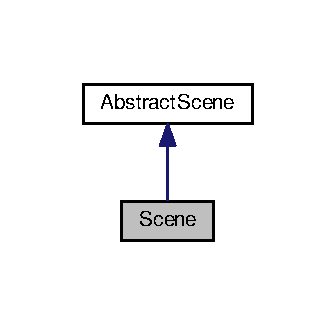
\includegraphics[width=161pt]{class_scene__inherit__graph}
\end{center}
\end{figure}


Collaboration diagram for Scene\+:
\nopagebreak
\begin{figure}[H]
\begin{center}
\leavevmode
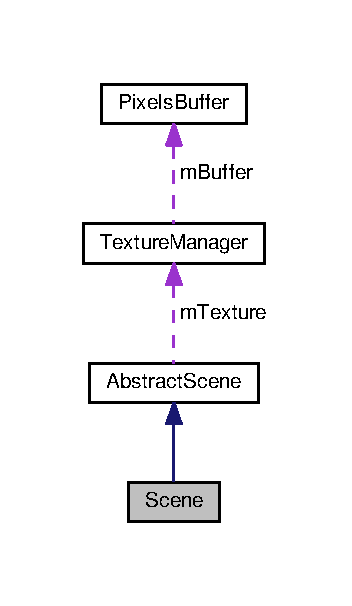
\includegraphics[width=169pt]{class_scene__coll__graph}
\end{center}
\end{figure}
\subsection*{Public Member Functions}
\begin{DoxyCompactItemize}
\item 
\hyperlink{class_scene_a91c732aff24d5b35d65a0f6e2fdfcd3a}{Scene} (const std\+::string path, const std\+::string texture, bool reshape=false)
\item 
virtual \hyperlink{class_scene_a3b8cec2e32546713915f8c6303c951f1}{$\sim$\+Scene} ()
\item 
void \hyperlink{class_scene_a4ddf2d16f371ee9533b3faf1dd5ddfb1}{render} ()
\begin{DoxyCompactList}\small\item\em Affiche la scene courante. \end{DoxyCompactList}\item 
void \hyperlink{class_scene_af0747116905b9098ba3bd2c9d4b67162}{render} (\hyperlink{class_noeud}{Noeud} noeud)
\item 
void \hyperlink{class_scene_a1184bf60ec953a9ae9f6b979cfcc8f69}{center} ()
\item 
\hyperlink{class_noeud}{Noeud} \hyperlink{class_scene_a6d9239ca059ca24b0a767aebc1c9a63b}{get\+Racine} ()
\begin{DoxyCompactList}\small\item\em Recupere le noeud mere de la scene. \end{DoxyCompactList}\item 
\hyperlink{class_vecteur3_d}{Vecteur3\+D} \hyperlink{class_scene_ada5afef61a8061abb6d3dfb38802f551}{get\+Center} ()
\begin{DoxyCompactList}\small\item\em Renvoie le center de la scene. \end{DoxyCompactList}\item 
std\+::vector$<$ \hyperlink{class_vecteur3_d}{Vecteur3\+D} $>$ \hyperlink{class_scene_a899e0ef799504383505743ebecc58406}{get\+Vertices} ()
\begin{DoxyCompactList}\small\item\em Renvoie la liste des vertices de la scene. \end{DoxyCompactList}\item 
std\+::vector$<$ \hyperlink{class_vecteur3_d}{Vecteur3\+D} $>$ \hyperlink{class_scene_a98442b4ed5ff289a695d9a6eea7b6ebd}{get\+Normals} ()
\begin{DoxyCompactList}\small\item\em Revoie la liste des normales de la scene. \end{DoxyCompactList}\end{DoxyCompactItemize}
\subsection*{Additional Inherited Members}


\subsection{Detailed Description}
\hyperlink{class_scene}{Scene} chargee par fichier 

\subsection{Constructor \& Destructor Documentation}
\hypertarget{class_scene_a91c732aff24d5b35d65a0f6e2fdfcd3a}{\index{Scene@{Scene}!Scene@{Scene}}
\index{Scene@{Scene}!Scene@{Scene}}
\subsubsection[{Scene}]{\setlength{\rightskip}{0pt plus 5cm}Scene\+::\+Scene (
\begin{DoxyParamCaption}
\item[{const std\+::string}]{path, }
\item[{const std\+::string}]{texture, }
\item[{bool}]{reshape = {\ttfamily false}}
\end{DoxyParamCaption}
)}}\label{class_scene_a91c732aff24d5b35d65a0f6e2fdfcd3a}
\hypertarget{class_scene_a3b8cec2e32546713915f8c6303c951f1}{\index{Scene@{Scene}!````~Scene@{$\sim$\+Scene}}
\index{````~Scene@{$\sim$\+Scene}!Scene@{Scene}}
\subsubsection[{$\sim$\+Scene}]{\setlength{\rightskip}{0pt plus 5cm}Scene\+::$\sim$\+Scene (
\begin{DoxyParamCaption}
{}
\end{DoxyParamCaption}
)\hspace{0.3cm}{\ttfamily [virtual]}}}\label{class_scene_a3b8cec2e32546713915f8c6303c951f1}


\subsection{Member Function Documentation}
\hypertarget{class_scene_a1184bf60ec953a9ae9f6b979cfcc8f69}{\index{Scene@{Scene}!center@{center}}
\index{center@{center}!Scene@{Scene}}
\subsubsection[{center}]{\setlength{\rightskip}{0pt plus 5cm}void Scene\+::center (
\begin{DoxyParamCaption}
{}
\end{DoxyParamCaption}
)}}\label{class_scene_a1184bf60ec953a9ae9f6b979cfcc8f69}
\hypertarget{class_scene_ada5afef61a8061abb6d3dfb38802f551}{\index{Scene@{Scene}!get\+Center@{get\+Center}}
\index{get\+Center@{get\+Center}!Scene@{Scene}}
\subsubsection[{get\+Center}]{\setlength{\rightskip}{0pt plus 5cm}{\bf Vecteur3\+D} Scene\+::get\+Center (
\begin{DoxyParamCaption}
{}
\end{DoxyParamCaption}
)\hspace{0.3cm}{\ttfamily [inline]}}}\label{class_scene_ada5afef61a8061abb6d3dfb38802f551}


Renvoie le center de la scene. 

\hypertarget{class_scene_a98442b4ed5ff289a695d9a6eea7b6ebd}{\index{Scene@{Scene}!get\+Normals@{get\+Normals}}
\index{get\+Normals@{get\+Normals}!Scene@{Scene}}
\subsubsection[{get\+Normals}]{\setlength{\rightskip}{0pt plus 5cm}std\+::vector$<$ {\bf Vecteur3\+D} $>$ Scene\+::get\+Normals (
\begin{DoxyParamCaption}
{}
\end{DoxyParamCaption}
)}}\label{class_scene_a98442b4ed5ff289a695d9a6eea7b6ebd}


Revoie la liste des normales de la scene. 

\hypertarget{class_scene_a6d9239ca059ca24b0a767aebc1c9a63b}{\index{Scene@{Scene}!get\+Racine@{get\+Racine}}
\index{get\+Racine@{get\+Racine}!Scene@{Scene}}
\subsubsection[{get\+Racine}]{\setlength{\rightskip}{0pt plus 5cm}{\bf Noeud} Scene\+::get\+Racine (
\begin{DoxyParamCaption}
{}
\end{DoxyParamCaption}
)}}\label{class_scene_a6d9239ca059ca24b0a767aebc1c9a63b}


Recupere le noeud mere de la scene. 

\begin{DoxyReturn}{Returns}
le \hyperlink{class_noeud}{Noeud} mere 
\end{DoxyReturn}
\hypertarget{class_scene_a899e0ef799504383505743ebecc58406}{\index{Scene@{Scene}!get\+Vertices@{get\+Vertices}}
\index{get\+Vertices@{get\+Vertices}!Scene@{Scene}}
\subsubsection[{get\+Vertices}]{\setlength{\rightskip}{0pt plus 5cm}std\+::vector$<$ {\bf Vecteur3\+D} $>$ Scene\+::get\+Vertices (
\begin{DoxyParamCaption}
{}
\end{DoxyParamCaption}
)}}\label{class_scene_a899e0ef799504383505743ebecc58406}


Renvoie la liste des vertices de la scene. 

\hypertarget{class_scene_a4ddf2d16f371ee9533b3faf1dd5ddfb1}{\index{Scene@{Scene}!render@{render}}
\index{render@{render}!Scene@{Scene}}
\subsubsection[{render}]{\setlength{\rightskip}{0pt plus 5cm}void Scene\+::render (
\begin{DoxyParamCaption}
{}
\end{DoxyParamCaption}
)\hspace{0.3cm}{\ttfamily [virtual]}}}\label{class_scene_a4ddf2d16f371ee9533b3faf1dd5ddfb1}


Affiche la scene courante. 



Reimplemented from \hyperlink{class_abstract_scene_aaf2f4c7aa4a6401f66bed00a51d8e64f}{Abstract\+Scene}.

\hypertarget{class_scene_af0747116905b9098ba3bd2c9d4b67162}{\index{Scene@{Scene}!render@{render}}
\index{render@{render}!Scene@{Scene}}
\subsubsection[{render}]{\setlength{\rightskip}{0pt plus 5cm}void Scene\+::render (
\begin{DoxyParamCaption}
\item[{{\bf Noeud}}]{noeud}
\end{DoxyParamCaption}
)}}\label{class_scene_af0747116905b9098ba3bd2c9d4b67162}


The documentation for this class was generated from the following files\+:\begin{DoxyCompactItemize}
\item 
src/\hyperlink{scene_8hpp}{scene.\+hpp}\item 
src/\hyperlink{scene_8cpp}{scene.\+cpp}\end{DoxyCompactItemize}

\hypertarget{class_systeme_solaire}{\section{Systeme\+Solaire Class Reference}
\label{class_systeme_solaire}\index{Systeme\+Solaire@{Systeme\+Solaire}}
}


{\ttfamily \#include $<$computed\+Scene.\+hpp$>$}



Inheritance diagram for Systeme\+Solaire\+:
\nopagebreak
\begin{figure}[H]
\begin{center}
\leavevmode
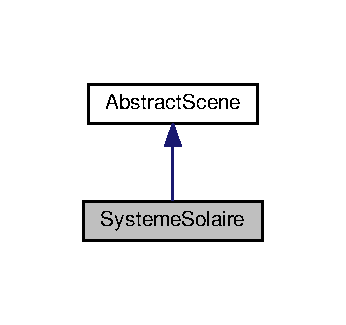
\includegraphics[width=166pt]{class_systeme_solaire__inherit__graph}
\end{center}
\end{figure}


Collaboration diagram for Systeme\+Solaire\+:
\nopagebreak
\begin{figure}[H]
\begin{center}
\leavevmode
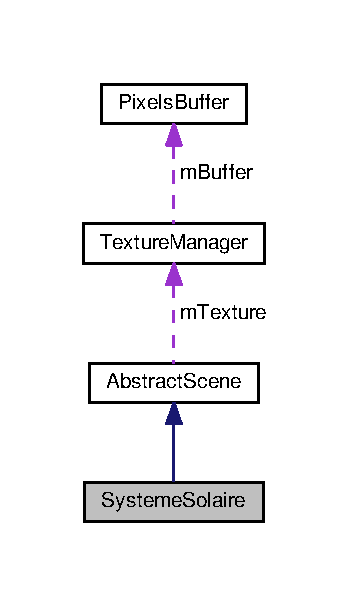
\includegraphics[width=169pt]{class_systeme_solaire__coll__graph}
\end{center}
\end{figure}
\subsection*{Public Member Functions}
\begin{DoxyCompactItemize}
\item 
\hyperlink{class_systeme_solaire_abaac51f06025a687641f20af2e82b22f}{Systeme\+Solaire} (int rayon\+Soleil)
\begin{DoxyCompactList}\small\item\em Etat de la rotation actuelle de la planete autour du soleil. \end{DoxyCompactList}\item 
\hyperlink{class_systeme_solaire_a8666eef6941cc92e325c2fa2eaa186f2}{$\sim$\+Systeme\+Solaire} ()
\item 
void \hyperlink{class_systeme_solaire_a500de47c923d4284867416bc007b9c11}{render} ()
\begin{DoxyCompactList}\small\item\em Affiche la scene courante. \end{DoxyCompactList}\end{DoxyCompactItemize}
\subsection*{Additional Inherited Members}


\subsection{Detailed Description}
\hyperlink{class_scene}{Scene} renvoyant un systeme solaire anime par transformation, calculee par Open\+G\+L 

\subsection{Constructor \& Destructor Documentation}
\hypertarget{class_systeme_solaire_abaac51f06025a687641f20af2e82b22f}{\index{Systeme\+Solaire@{Systeme\+Solaire}!Systeme\+Solaire@{Systeme\+Solaire}}
\index{Systeme\+Solaire@{Systeme\+Solaire}!Systeme\+Solaire@{Systeme\+Solaire}}
\subsubsection[{Systeme\+Solaire}]{\setlength{\rightskip}{0pt plus 5cm}Systeme\+Solaire\+::\+Systeme\+Solaire (
\begin{DoxyParamCaption}
\item[{int}]{rayon\+Soleil}
\end{DoxyParamCaption}
)\hspace{0.3cm}{\ttfamily [inline]}}}\label{class_systeme_solaire_abaac51f06025a687641f20af2e82b22f}


Etat de la rotation actuelle de la planete autour du soleil. 

\hypertarget{class_systeme_solaire_a8666eef6941cc92e325c2fa2eaa186f2}{\index{Systeme\+Solaire@{Systeme\+Solaire}!````~Systeme\+Solaire@{$\sim$\+Systeme\+Solaire}}
\index{````~Systeme\+Solaire@{$\sim$\+Systeme\+Solaire}!Systeme\+Solaire@{Systeme\+Solaire}}
\subsubsection[{$\sim$\+Systeme\+Solaire}]{\setlength{\rightskip}{0pt plus 5cm}Systeme\+Solaire\+::$\sim$\+Systeme\+Solaire (
\begin{DoxyParamCaption}
{}
\end{DoxyParamCaption}
)\hspace{0.3cm}{\ttfamily [inline]}}}\label{class_systeme_solaire_a8666eef6941cc92e325c2fa2eaa186f2}


\subsection{Member Function Documentation}
\hypertarget{class_systeme_solaire_a500de47c923d4284867416bc007b9c11}{\index{Systeme\+Solaire@{Systeme\+Solaire}!render@{render}}
\index{render@{render}!Systeme\+Solaire@{Systeme\+Solaire}}
\subsubsection[{render}]{\setlength{\rightskip}{0pt plus 5cm}void Systeme\+Solaire\+::render (
\begin{DoxyParamCaption}
{}
\end{DoxyParamCaption}
)\hspace{0.3cm}{\ttfamily [virtual]}}}\label{class_systeme_solaire_a500de47c923d4284867416bc007b9c11}


Affiche la scene courante. 



Reimplemented from \hyperlink{class_abstract_scene_aaf2f4c7aa4a6401f66bed00a51d8e64f}{Abstract\+Scene}.



The documentation for this class was generated from the following files\+:\begin{DoxyCompactItemize}
\item 
src/\hyperlink{computed_scene_8hpp}{computed\+Scene.\+hpp}\item 
src/\hyperlink{computed_scene_8cpp}{computed\+Scene.\+cpp}\end{DoxyCompactItemize}

\hypertarget{class_teapot}{}\section{Teapot Class Reference}
\label{class_teapot}\index{Teapot@{Teapot}}


{\ttfamily \#include $<$computed\+Scene.\+hpp$>$}



Inheritance diagram for Teapot\+:
% FIG 0


Collaboration diagram for Teapot\+:
% FIG 1
\subsection*{Public Member Functions}
\begin{DoxyCompactItemize}
\item 
\hyperlink{class_teapot_a31d8fcc65137fb5ff8d958667e7675a4}{Teapot} (int size)
\item 
\hyperlink{class_teapot_a1c243d488157da74b0e1a2412a921f00}{$\sim$\+Teapot} ()
\item 
void \hyperlink{class_teapot_aababf7bd2833ebd3c34564b45b902163}{render} ()
\end{DoxyCompactItemize}
\subsection*{Additional Inherited Members}


\subsection{Constructor \& Destructor Documentation}
\index{Teapot@{Teapot}!Teapot@{Teapot}}
\index{Teapot@{Teapot}!Teapot@{Teapot}}
\subsubsection[{\texorpdfstring{Teapot(int size)}{Teapot(int size)}}]{\setlength{\rightskip}{0pt plus 5cm}Teapot\+::\+Teapot (
\begin{DoxyParamCaption}
\item[{int}]{size}
\end{DoxyParamCaption}
)\hspace{0.3cm}{\ttfamily [inline]}}\hypertarget{class_teapot_a31d8fcc65137fb5ff8d958667e7675a4}{}\label{class_teapot_a31d8fcc65137fb5ff8d958667e7675a4}
\index{Teapot@{Teapot}!````~Teapot@{$\sim$\+Teapot}}
\index{````~Teapot@{$\sim$\+Teapot}!Teapot@{Teapot}}
\subsubsection[{\texorpdfstring{$\sim$\+Teapot()}{~Teapot()}}]{\setlength{\rightskip}{0pt plus 5cm}Teapot\+::$\sim$\+Teapot (
\begin{DoxyParamCaption}
{}
\end{DoxyParamCaption}
)\hspace{0.3cm}{\ttfamily [inline]}}\hypertarget{class_teapot_a1c243d488157da74b0e1a2412a921f00}{}\label{class_teapot_a1c243d488157da74b0e1a2412a921f00}


\subsection{Member Function Documentation}
\index{Teapot@{Teapot}!render@{render}}
\index{render@{render}!Teapot@{Teapot}}
\subsubsection[{\texorpdfstring{render()}{render()}}]{\setlength{\rightskip}{0pt plus 5cm}void Teapot\+::render (
\begin{DoxyParamCaption}
{}
\end{DoxyParamCaption}
)\hspace{0.3cm}{\ttfamily [virtual]}}\hypertarget{class_teapot_aababf7bd2833ebd3c34564b45b902163}{}\label{class_teapot_aababf7bd2833ebd3c34564b45b902163}


Implements \hyperlink{class_abstract_scene_ae4f545c8335b65b42a6198ee09bf8084}{Abstract\+Scene}.



The documentation for this class was generated from the following files\+:\begin{DoxyCompactItemize}
\item 
architecture/\hyperlink{computed_scene_8hpp}{computed\+Scene.\+hpp}\item 
architecture/\hyperlink{computed_scene_8cpp}{computed\+Scene.\+cpp}\end{DoxyCompactItemize}

\hypertarget{class_transfo_camera}{\section{Transfo\+Camera Class Reference}
\label{class_transfo_camera}\index{Transfo\+Camera@{Transfo\+Camera}}
}


{\ttfamily \#include $<$transfo\+Camera.\+hpp$>$}



Inheritance diagram for Transfo\+Camera\+:
\nopagebreak
\begin{figure}[H]
\begin{center}
\leavevmode
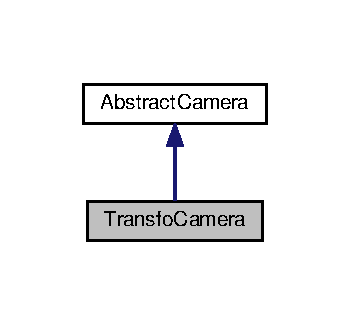
\includegraphics[width=168pt]{class_transfo_camera__inherit__graph}
\end{center}
\end{figure}


Collaboration diagram for Transfo\+Camera\+:
\nopagebreak
\begin{figure}[H]
\begin{center}
\leavevmode
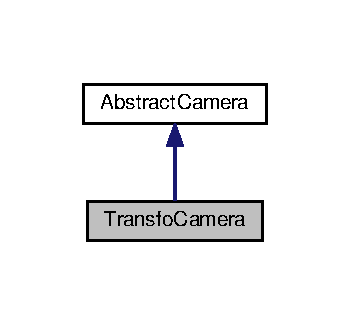
\includegraphics[width=168pt]{class_transfo_camera__coll__graph}
\end{center}
\end{figure}
\subsection*{Public Member Functions}
\begin{DoxyCompactItemize}
\item 
\hyperlink{class_transfo_camera_a3543cac1c73f91389a7509c6a6baf5f2}{Transfo\+Camera} (double px, double py, double pz, double vx, double vy, double vz, double vertx, double verty, double vertz, double zproche=1, double zeloigne=500, double angle\+Ouverture=50, double azimuth=0.\+0, double elevation=0.\+0)
\item 
virtual \hyperlink{class_transfo_camera_af1f4189a386127ee63b29b392c0a8b41}{$\sim$\+Transfo\+Camera} ()
\item 
virtual void \hyperlink{class_transfo_camera_af56c28b564652b71b7040084aaec8ff9}{Changer\+Repere\+Camera} (double position\mbox{[}3\mbox{]}, double point\+De\+Visee\mbox{[}3\mbox{]}, double vecteur\+Vertical\mbox{[}3\mbox{]})
\begin{DoxyCompactList}\small\item\em Changement du repère de la caméra. \end{DoxyCompactList}\item 
virtual void \hyperlink{class_transfo_camera_a1d02bd6398256954713d1c239d2ebcba}{Changer\+Repere\+Camera} ()
\begin{DoxyCompactList}\small\item\em Changement du repère de la caméra. \end{DoxyCompactList}\item 
void \hyperlink{class_transfo_camera_af6df80037a1b33cecd28672255c38f1f}{Set\+Azimuth} (double a)
\begin{DoxyCompactList}\small\item\em Setter de l'angle azimuth. \end{DoxyCompactList}\item 
void \hyperlink{class_transfo_camera_a4e1dc4a565df1976c07ebbbf011427b8}{Set\+Elevation} (double e)
\begin{DoxyCompactList}\small\item\em Setter de l'angle d'élévation. \end{DoxyCompactList}\item 
double \hyperlink{class_transfo_camera_a8c2f48af070cc18d0f0c33cb3edbcf72}{Get\+Azimuth} (void) const 
\begin{DoxyCompactList}\small\item\em Getter de l'angle azimuth. \end{DoxyCompactList}\item 
double \hyperlink{class_transfo_camera_aed836872b472780c197b9fd3f4b4f1a8}{Get\+Elevation} (void) const 
\begin{DoxyCompactList}\small\item\em Getter de l'angle d'élévation. \end{DoxyCompactList}\end{DoxyCompactItemize}
\subsection*{Protected Attributes}
\begin{DoxyCompactItemize}
\item 
double \hyperlink{class_transfo_camera_a6856f4b9d2af270afbb0c40bd23a7fa6}{m\+Azimuth}
\item 
double \hyperlink{class_transfo_camera_ac6afc5482df198c3a311fa02a74680e5}{m\+Elevation}
\end{DoxyCompactItemize}
\subsection*{Additional Inherited Members}


\subsection{Constructor \& Destructor Documentation}
\hypertarget{class_transfo_camera_a3543cac1c73f91389a7509c6a6baf5f2}{\index{Transfo\+Camera@{Transfo\+Camera}!Transfo\+Camera@{Transfo\+Camera}}
\index{Transfo\+Camera@{Transfo\+Camera}!Transfo\+Camera@{Transfo\+Camera}}
\subsubsection[{Transfo\+Camera}]{\setlength{\rightskip}{0pt plus 5cm}Transfo\+Camera\+::\+Transfo\+Camera (
\begin{DoxyParamCaption}
\item[{double}]{px, }
\item[{double}]{py, }
\item[{double}]{pz, }
\item[{double}]{vx, }
\item[{double}]{vy, }
\item[{double}]{vz, }
\item[{double}]{vertx, }
\item[{double}]{verty, }
\item[{double}]{vertz, }
\item[{double}]{zproche = {\ttfamily 1}, }
\item[{double}]{zeloigne = {\ttfamily 500}, }
\item[{double}]{angle\+Ouverture = {\ttfamily 50}, }
\item[{double}]{azimuth = {\ttfamily 0.0}, }
\item[{double}]{elevation = {\ttfamily 0.0}}
\end{DoxyParamCaption}
)}}\label{class_transfo_camera_a3543cac1c73f91389a7509c6a6baf5f2}
'Default' constructor \hypertarget{class_transfo_camera_af1f4189a386127ee63b29b392c0a8b41}{\index{Transfo\+Camera@{Transfo\+Camera}!````~Transfo\+Camera@{$\sim$\+Transfo\+Camera}}
\index{````~Transfo\+Camera@{$\sim$\+Transfo\+Camera}!Transfo\+Camera@{Transfo\+Camera}}
\subsubsection[{$\sim$\+Transfo\+Camera}]{\setlength{\rightskip}{0pt plus 5cm}Transfo\+Camera\+::$\sim$\+Transfo\+Camera (
\begin{DoxyParamCaption}
{}
\end{DoxyParamCaption}
)\hspace{0.3cm}{\ttfamily [virtual]}}}\label{class_transfo_camera_af1f4189a386127ee63b29b392c0a8b41}
Default destructor 

\subsection{Member Function Documentation}
\hypertarget{class_transfo_camera_af56c28b564652b71b7040084aaec8ff9}{\index{Transfo\+Camera@{Transfo\+Camera}!Changer\+Repere\+Camera@{Changer\+Repere\+Camera}}
\index{Changer\+Repere\+Camera@{Changer\+Repere\+Camera}!Transfo\+Camera@{Transfo\+Camera}}
\subsubsection[{Changer\+Repere\+Camera}]{\setlength{\rightskip}{0pt plus 5cm}void Transfo\+Camera\+::\+Changer\+Repere\+Camera (
\begin{DoxyParamCaption}
\item[{double}]{position\mbox{[}3\mbox{]}, }
\item[{double}]{point\+De\+Visee\mbox{[}3\mbox{]}, }
\item[{double}]{vecteur\+Vertical\mbox{[}3\mbox{]}}
\end{DoxyParamCaption}
)\hspace{0.3cm}{\ttfamily [virtual]}}}\label{class_transfo_camera_af56c28b564652b71b7040084aaec8ff9}


Changement du repère de la caméra. 


\begin{DoxyParams}{Parameters}
{\em double\mbox{[}$\,$\mbox{]}} & position de la caméra \\
\hline
{\em double\mbox{[}$\,$\mbox{]}} & point de visée de la caméra \\
\hline
{\em double\mbox{[}$\,$\mbox{]}} & vertical de la caméra \\
\hline
\end{DoxyParams}
\begin{DoxyReturn}{Returns}
void 
\end{DoxyReturn}


Implements \hyperlink{class_abstract_camera_aeaa6522c54a923a50137d2c0ca54238b}{Abstract\+Camera}.

\hypertarget{class_transfo_camera_a1d02bd6398256954713d1c239d2ebcba}{\index{Transfo\+Camera@{Transfo\+Camera}!Changer\+Repere\+Camera@{Changer\+Repere\+Camera}}
\index{Changer\+Repere\+Camera@{Changer\+Repere\+Camera}!Transfo\+Camera@{Transfo\+Camera}}
\subsubsection[{Changer\+Repere\+Camera}]{\setlength{\rightskip}{0pt plus 5cm}void Transfo\+Camera\+::\+Changer\+Repere\+Camera (
\begin{DoxyParamCaption}
{}
\end{DoxyParamCaption}
)\hspace{0.3cm}{\ttfamily [virtual]}}}\label{class_transfo_camera_a1d02bd6398256954713d1c239d2ebcba}


Changement du repère de la caméra. 


\begin{DoxyParams}{Parameters}
{\em void} & \\
\hline
\end{DoxyParams}
\begin{DoxyReturn}{Returns}
void 
\end{DoxyReturn}


Implements \hyperlink{class_abstract_camera_a4bfcc6ed8980d64cf1d43d7dcb60129b}{Abstract\+Camera}.

\hypertarget{class_transfo_camera_a8c2f48af070cc18d0f0c33cb3edbcf72}{\index{Transfo\+Camera@{Transfo\+Camera}!Get\+Azimuth@{Get\+Azimuth}}
\index{Get\+Azimuth@{Get\+Azimuth}!Transfo\+Camera@{Transfo\+Camera}}
\subsubsection[{Get\+Azimuth}]{\setlength{\rightskip}{0pt plus 5cm}double Transfo\+Camera\+::\+Get\+Azimuth (
\begin{DoxyParamCaption}
\item[{void}]{}
\end{DoxyParamCaption}
) const}}\label{class_transfo_camera_a8c2f48af070cc18d0f0c33cb3edbcf72}


Getter de l'angle azimuth. 


\begin{DoxyParams}{Parameters}
{\em void} & \\
\hline
\end{DoxyParams}
\begin{DoxyReturn}{Returns}
double 
\end{DoxyReturn}
\hypertarget{class_transfo_camera_aed836872b472780c197b9fd3f4b4f1a8}{\index{Transfo\+Camera@{Transfo\+Camera}!Get\+Elevation@{Get\+Elevation}}
\index{Get\+Elevation@{Get\+Elevation}!Transfo\+Camera@{Transfo\+Camera}}
\subsubsection[{Get\+Elevation}]{\setlength{\rightskip}{0pt plus 5cm}double Transfo\+Camera\+::\+Get\+Elevation (
\begin{DoxyParamCaption}
\item[{void}]{}
\end{DoxyParamCaption}
) const}}\label{class_transfo_camera_aed836872b472780c197b9fd3f4b4f1a8}


Getter de l'angle d'élévation. 


\begin{DoxyParams}{Parameters}
{\em void} & \\
\hline
\end{DoxyParams}
\begin{DoxyReturn}{Returns}
double 
\end{DoxyReturn}
\hypertarget{class_transfo_camera_af6df80037a1b33cecd28672255c38f1f}{\index{Transfo\+Camera@{Transfo\+Camera}!Set\+Azimuth@{Set\+Azimuth}}
\index{Set\+Azimuth@{Set\+Azimuth}!Transfo\+Camera@{Transfo\+Camera}}
\subsubsection[{Set\+Azimuth}]{\setlength{\rightskip}{0pt plus 5cm}void Transfo\+Camera\+::\+Set\+Azimuth (
\begin{DoxyParamCaption}
\item[{double}]{a}
\end{DoxyParamCaption}
)}}\label{class_transfo_camera_af6df80037a1b33cecd28672255c38f1f}


Setter de l'angle azimuth. 


\begin{DoxyParams}{Parameters}
{\em double} & \+: nouvel angle \\
\hline
\end{DoxyParams}
\begin{DoxyReturn}{Returns}
void 
\end{DoxyReturn}
\hypertarget{class_transfo_camera_a4e1dc4a565df1976c07ebbbf011427b8}{\index{Transfo\+Camera@{Transfo\+Camera}!Set\+Elevation@{Set\+Elevation}}
\index{Set\+Elevation@{Set\+Elevation}!Transfo\+Camera@{Transfo\+Camera}}
\subsubsection[{Set\+Elevation}]{\setlength{\rightskip}{0pt plus 5cm}void Transfo\+Camera\+::\+Set\+Elevation (
\begin{DoxyParamCaption}
\item[{double}]{e}
\end{DoxyParamCaption}
)}}\label{class_transfo_camera_a4e1dc4a565df1976c07ebbbf011427b8}


Setter de l'angle d'élévation. 


\begin{DoxyParams}{Parameters}
{\em double} & \+: nouvel angle \\
\hline
\end{DoxyParams}
\begin{DoxyReturn}{Returns}
void 
\end{DoxyReturn}


\subsection{Member Data Documentation}
\hypertarget{class_transfo_camera_a6856f4b9d2af270afbb0c40bd23a7fa6}{\index{Transfo\+Camera@{Transfo\+Camera}!m\+Azimuth@{m\+Azimuth}}
\index{m\+Azimuth@{m\+Azimuth}!Transfo\+Camera@{Transfo\+Camera}}
\subsubsection[{m\+Azimuth}]{\setlength{\rightskip}{0pt plus 5cm}double Transfo\+Camera\+::m\+Azimuth\hspace{0.3cm}{\ttfamily [protected]}}}\label{class_transfo_camera_a6856f4b9d2af270afbb0c40bd23a7fa6}
\hypertarget{class_transfo_camera_ac6afc5482df198c3a311fa02a74680e5}{\index{Transfo\+Camera@{Transfo\+Camera}!m\+Elevation@{m\+Elevation}}
\index{m\+Elevation@{m\+Elevation}!Transfo\+Camera@{Transfo\+Camera}}
\subsubsection[{m\+Elevation}]{\setlength{\rightskip}{0pt plus 5cm}double Transfo\+Camera\+::m\+Elevation\hspace{0.3cm}{\ttfamily [protected]}}}\label{class_transfo_camera_ac6afc5482df198c3a311fa02a74680e5}


The documentation for this class was generated from the following files\+:\begin{DoxyCompactItemize}
\item 
src/\hyperlink{transfo_camera_8hpp}{transfo\+Camera.\+hpp}\item 
src/\hyperlink{transfo_camera_8cpp}{transfo\+Camera.\+cpp}\end{DoxyCompactItemize}

\hypertarget{class_vecteur3_d}{\section{Vecteur3\+D Class Reference}
\label{class_vecteur3_d}\index{Vecteur3\+D@{Vecteur3\+D}}
}


Classe pour un vecteur 3\+D Cette classe encapsule les ai\+Vector3\+D.  




{\ttfamily \#include $<$vecteur3\+D.\+hpp$>$}

\subsection*{Public Member Functions}
\begin{DoxyCompactItemize}
\item 
\hyperlink{class_vecteur3_d_aa2e1f3f01cadb1a3489ab0a5ee469b01}{Vecteur3\+D} (float x=0.\+0, float y=0.\+0, float z=0.\+0)
\begin{DoxyCompactList}\small\item\em Constructeur. \end{DoxyCompactList}\item 
\hyperlink{class_vecteur3_d_ad7960e596005df06dc7404f0ebb4ad89}{Vecteur3\+D} (const \hyperlink{class_vecteur3_d}{Vecteur3\+D} \&vec)
\begin{DoxyCompactList}\small\item\em Constructeur par copie. \end{DoxyCompactList}\item 
virtual \hyperlink{class_vecteur3_d_a5f4633710eef6f25175fb811bf811112}{$\sim$\+Vecteur3\+D} ()
\begin{DoxyCompactList}\small\item\em Destructeur. \end{DoxyCompactList}\item 
float \hyperlink{class_vecteur3_d_a3a5374f1fd023d46a517f0875ed0d865}{Get\+X} () const 
\begin{DoxyCompactList}\small\item\em Getter pour la coordonnée X. \end{DoxyCompactList}\item 
float \hyperlink{class_vecteur3_d_a160e036f4b71271fd375bc14b2e1e78c}{Get\+Y} () const 
\begin{DoxyCompactList}\small\item\em Getter pour la coordonnée Y. \end{DoxyCompactList}\item 
float \hyperlink{class_vecteur3_d_a001bd37a2d98c071b59d168057735eeb}{Get\+Z} () const 
\begin{DoxyCompactList}\small\item\em Getter pour la coordonnée Z. \end{DoxyCompactList}\item 
void \hyperlink{class_vecteur3_d_a9e987e98ee43903a5281752bd310a764}{Set\+X} (float)
\begin{DoxyCompactList}\small\item\em Setter pour la coordonnée X. \end{DoxyCompactList}\item 
void \hyperlink{class_vecteur3_d_aaef5dfb35864a47ac7eb986cead20c71}{Set\+Y} (float)
\begin{DoxyCompactList}\small\item\em Setter pour la coordonnée Y. \end{DoxyCompactList}\item 
void \hyperlink{class_vecteur3_d_a0b20935a9e30452ea51da98fc8878181}{Set\+Z} (float)
\begin{DoxyCompactList}\small\item\em Setter pour la coordonnée Z. \end{DoxyCompactList}\item 
\hyperlink{class_vecteur3_d}{Vecteur3\+D} \hyperlink{class_vecteur3_d_a3da112b573b37eb696dd17c7f3a4230f}{Normalize} () const 
\begin{DoxyCompactList}\small\item\em Calcul le vecteur normalisé \end{DoxyCompactList}\item 
\hyperlink{class_vecteur3_d}{Vecteur3\+D} \hyperlink{class_vecteur3_d_a7050066f71a250c11b81e58e1466b389}{Cross} (\hyperlink{class_vecteur3_d}{Vecteur3\+D} v) const 
\begin{DoxyCompactList}\small\item\em Calcul le produit vectoriel. \end{DoxyCompactList}\item 
float \hyperlink{class_vecteur3_d_aa428d49b67ee120ae871cec35fd43805}{Dot} (\hyperlink{class_vecteur3_d}{Vecteur3\+D} \&v) const 
\begin{DoxyCompactList}\small\item\em Calcul le produit scalaire. \end{DoxyCompactList}\end{DoxyCompactItemize}


\subsection{Detailed Description}
Classe pour un vecteur 3\+D Cette classe encapsule les ai\+Vector3\+D. 

\subsection{Constructor \& Destructor Documentation}
\hypertarget{class_vecteur3_d_aa2e1f3f01cadb1a3489ab0a5ee469b01}{\index{Vecteur3\+D@{Vecteur3\+D}!Vecteur3\+D@{Vecteur3\+D}}
\index{Vecteur3\+D@{Vecteur3\+D}!Vecteur3\+D@{Vecteur3\+D}}
\subsubsection[{Vecteur3\+D}]{\setlength{\rightskip}{0pt plus 5cm}Vecteur3\+D\+::\+Vecteur3\+D (
\begin{DoxyParamCaption}
\item[{float}]{x = {\ttfamily 0.0}, }
\item[{float}]{y = {\ttfamily 0.0}, }
\item[{float}]{z = {\ttfamily 0.0}}
\end{DoxyParamCaption}
)}}\label{class_vecteur3_d_aa2e1f3f01cadb1a3489ab0a5ee469b01}


Constructeur. 


\begin{DoxyParams}{Parameters}
{\em Cooronnée} & x (0 par défaut) \\
\hline
{\em Cooronnée} & y (0 par défaut) \\
\hline
{\em Cooronnée} & z (0 par défaut) \\
\hline
\end{DoxyParams}
\hypertarget{class_vecteur3_d_ad7960e596005df06dc7404f0ebb4ad89}{\index{Vecteur3\+D@{Vecteur3\+D}!Vecteur3\+D@{Vecteur3\+D}}
\index{Vecteur3\+D@{Vecteur3\+D}!Vecteur3\+D@{Vecteur3\+D}}
\subsubsection[{Vecteur3\+D}]{\setlength{\rightskip}{0pt plus 5cm}Vecteur3\+D\+::\+Vecteur3\+D (
\begin{DoxyParamCaption}
\item[{const {\bf Vecteur3\+D} \&}]{vec}
\end{DoxyParamCaption}
)}}\label{class_vecteur3_d_ad7960e596005df06dc7404f0ebb4ad89}


Constructeur par copie. 

\hypertarget{class_vecteur3_d_a5f4633710eef6f25175fb811bf811112}{\index{Vecteur3\+D@{Vecteur3\+D}!````~Vecteur3\+D@{$\sim$\+Vecteur3\+D}}
\index{````~Vecteur3\+D@{$\sim$\+Vecteur3\+D}!Vecteur3\+D@{Vecteur3\+D}}
\subsubsection[{$\sim$\+Vecteur3\+D}]{\setlength{\rightskip}{0pt plus 5cm}Vecteur3\+D\+::$\sim$\+Vecteur3\+D (
\begin{DoxyParamCaption}
{}
\end{DoxyParamCaption}
)\hspace{0.3cm}{\ttfamily [virtual]}}}\label{class_vecteur3_d_a5f4633710eef6f25175fb811bf811112}


Destructeur. 



\subsection{Member Function Documentation}
\hypertarget{class_vecteur3_d_a7050066f71a250c11b81e58e1466b389}{\index{Vecteur3\+D@{Vecteur3\+D}!Cross@{Cross}}
\index{Cross@{Cross}!Vecteur3\+D@{Vecteur3\+D}}
\subsubsection[{Cross}]{\setlength{\rightskip}{0pt plus 5cm}{\bf Vecteur3\+D} Vecteur3\+D\+::\+Cross (
\begin{DoxyParamCaption}
\item[{{\bf Vecteur3\+D}}]{v}
\end{DoxyParamCaption}
) const}}\label{class_vecteur3_d_a7050066f71a250c11b81e58e1466b389}


Calcul le produit vectoriel. 


\begin{DoxyParams}{Parameters}
{\em Un} & \hyperlink{class_vecteur3_d}{Vecteur3\+D} pour le produit. \\
\hline
\end{DoxyParams}
\begin{DoxyReturn}{Returns}
Un \hyperlink{class_vecteur3_d}{Vecteur3\+D} contenant le vecteur produit. 
\end{DoxyReturn}
\hypertarget{class_vecteur3_d_aa428d49b67ee120ae871cec35fd43805}{\index{Vecteur3\+D@{Vecteur3\+D}!Dot@{Dot}}
\index{Dot@{Dot}!Vecteur3\+D@{Vecteur3\+D}}
\subsubsection[{Dot}]{\setlength{\rightskip}{0pt plus 5cm}float Vecteur3\+D\+::\+Dot (
\begin{DoxyParamCaption}
\item[{{\bf Vecteur3\+D} \&}]{v}
\end{DoxyParamCaption}
) const}}\label{class_vecteur3_d_aa428d49b67ee120ae871cec35fd43805}


Calcul le produit scalaire. 


\begin{DoxyParams}{Parameters}
{\em Un} & \hyperlink{class_vecteur3_d}{Vecteur3\+D} pour le produit. \\
\hline
\end{DoxyParams}
\begin{DoxyReturn}{Returns}
Un float contenant le résultat. 
\end{DoxyReturn}
\hypertarget{class_vecteur3_d_a3a5374f1fd023d46a517f0875ed0d865}{\index{Vecteur3\+D@{Vecteur3\+D}!Get\+X@{Get\+X}}
\index{Get\+X@{Get\+X}!Vecteur3\+D@{Vecteur3\+D}}
\subsubsection[{Get\+X}]{\setlength{\rightskip}{0pt plus 5cm}float Vecteur3\+D\+::\+Get\+X (
\begin{DoxyParamCaption}
{}
\end{DoxyParamCaption}
) const}}\label{class_vecteur3_d_a3a5374f1fd023d46a517f0875ed0d865}


Getter pour la coordonnée X. 

\begin{DoxyReturn}{Returns}
Un float. 
\end{DoxyReturn}
\hypertarget{class_vecteur3_d_a160e036f4b71271fd375bc14b2e1e78c}{\index{Vecteur3\+D@{Vecteur3\+D}!Get\+Y@{Get\+Y}}
\index{Get\+Y@{Get\+Y}!Vecteur3\+D@{Vecteur3\+D}}
\subsubsection[{Get\+Y}]{\setlength{\rightskip}{0pt plus 5cm}float Vecteur3\+D\+::\+Get\+Y (
\begin{DoxyParamCaption}
{}
\end{DoxyParamCaption}
) const}}\label{class_vecteur3_d_a160e036f4b71271fd375bc14b2e1e78c}


Getter pour la coordonnée Y. 

\begin{DoxyReturn}{Returns}
Un float. 
\end{DoxyReturn}
\hypertarget{class_vecteur3_d_a001bd37a2d98c071b59d168057735eeb}{\index{Vecteur3\+D@{Vecteur3\+D}!Get\+Z@{Get\+Z}}
\index{Get\+Z@{Get\+Z}!Vecteur3\+D@{Vecteur3\+D}}
\subsubsection[{Get\+Z}]{\setlength{\rightskip}{0pt plus 5cm}float Vecteur3\+D\+::\+Get\+Z (
\begin{DoxyParamCaption}
{}
\end{DoxyParamCaption}
) const}}\label{class_vecteur3_d_a001bd37a2d98c071b59d168057735eeb}


Getter pour la coordonnée Z. 

\begin{DoxyReturn}{Returns}
Un float. 
\end{DoxyReturn}
\hypertarget{class_vecteur3_d_a3da112b573b37eb696dd17c7f3a4230f}{\index{Vecteur3\+D@{Vecteur3\+D}!Normalize@{Normalize}}
\index{Normalize@{Normalize}!Vecteur3\+D@{Vecteur3\+D}}
\subsubsection[{Normalize}]{\setlength{\rightskip}{0pt plus 5cm}{\bf Vecteur3\+D} Vecteur3\+D\+::\+Normalize (
\begin{DoxyParamCaption}
{}
\end{DoxyParamCaption}
) const}}\label{class_vecteur3_d_a3da112b573b37eb696dd17c7f3a4230f}


Calcul le vecteur normalisé 

\begin{DoxyReturn}{Returns}
Un \hyperlink{class_vecteur3_d}{Vecteur3\+D} contenant le vecteur normalisé. 
\end{DoxyReturn}
\hypertarget{class_vecteur3_d_a9e987e98ee43903a5281752bd310a764}{\index{Vecteur3\+D@{Vecteur3\+D}!Set\+X@{Set\+X}}
\index{Set\+X@{Set\+X}!Vecteur3\+D@{Vecteur3\+D}}
\subsubsection[{Set\+X}]{\setlength{\rightskip}{0pt plus 5cm}void Vecteur3\+D\+::\+Set\+X (
\begin{DoxyParamCaption}
\item[{float}]{new\+X}
\end{DoxyParamCaption}
)}}\label{class_vecteur3_d_a9e987e98ee43903a5281752bd310a764}


Setter pour la coordonnée X. 


\begin{DoxyParams}{Parameters}
{\em Un} & float. \\
\hline
\end{DoxyParams}
\hypertarget{class_vecteur3_d_aaef5dfb35864a47ac7eb986cead20c71}{\index{Vecteur3\+D@{Vecteur3\+D}!Set\+Y@{Set\+Y}}
\index{Set\+Y@{Set\+Y}!Vecteur3\+D@{Vecteur3\+D}}
\subsubsection[{Set\+Y}]{\setlength{\rightskip}{0pt plus 5cm}void Vecteur3\+D\+::\+Set\+Y (
\begin{DoxyParamCaption}
\item[{float}]{new\+Y}
\end{DoxyParamCaption}
)}}\label{class_vecteur3_d_aaef5dfb35864a47ac7eb986cead20c71}


Setter pour la coordonnée Y. 


\begin{DoxyParams}{Parameters}
{\em Un} & float. \\
\hline
\end{DoxyParams}
\hypertarget{class_vecteur3_d_a0b20935a9e30452ea51da98fc8878181}{\index{Vecteur3\+D@{Vecteur3\+D}!Set\+Z@{Set\+Z}}
\index{Set\+Z@{Set\+Z}!Vecteur3\+D@{Vecteur3\+D}}
\subsubsection[{Set\+Z}]{\setlength{\rightskip}{0pt plus 5cm}void Vecteur3\+D\+::\+Set\+Z (
\begin{DoxyParamCaption}
\item[{float}]{new\+Z}
\end{DoxyParamCaption}
)}}\label{class_vecteur3_d_a0b20935a9e30452ea51da98fc8878181}


Setter pour la coordonnée Z. 


\begin{DoxyParams}{Parameters}
{\em Un} & float. \\
\hline
\end{DoxyParams}


The documentation for this class was generated from the following files\+:\begin{DoxyCompactItemize}
\item 
src/\hyperlink{vecteur3_d_8hpp}{vecteur3\+D.\+hpp}\item 
src/\hyperlink{vecteur3_d_8cpp}{vecteur3\+D.\+cpp}\end{DoxyCompactItemize}

\hypertarget{class_voiture}{\section{Voiture Class Reference}
\label{class_voiture}\index{Voiture@{Voiture}}
}


{\ttfamily \#include $<$computed\+Scene.\+hpp$>$}



Inheritance diagram for Voiture\+:
\nopagebreak
\begin{figure}[H]
\begin{center}
\leavevmode
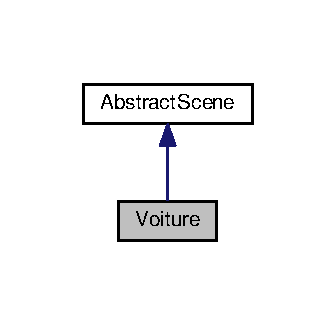
\includegraphics[width=161pt]{class_voiture__inherit__graph}
\end{center}
\end{figure}


Collaboration diagram for Voiture\+:
\nopagebreak
\begin{figure}[H]
\begin{center}
\leavevmode
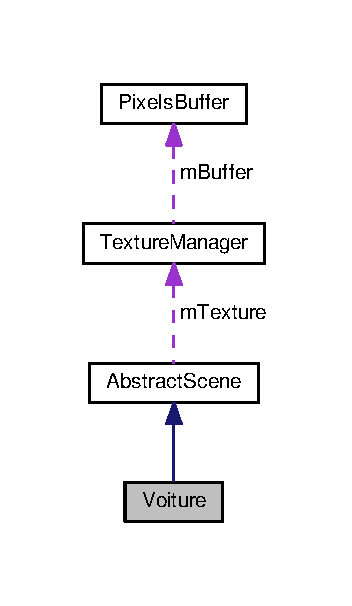
\includegraphics[width=169pt]{class_voiture__coll__graph}
\end{center}
\end{figure}
\subsection*{Public Member Functions}
\begin{DoxyCompactItemize}
\item 
\hyperlink{class_voiture_a566a3faabc5c390003fa46988e5928a1}{Voiture} (double vitesse\+Roue=0.\+1)
\begin{DoxyCompactList}\small\item\em etat max de la rotaiton des roues \end{DoxyCompactList}\item 
\hyperlink{class_voiture_afe85820a993b6908d0fdb524245e5133}{$\sim$\+Voiture} ()
\item 
void \hyperlink{class_voiture_a6232a9043c077a4f69e92b90566d9b78}{draw\+Roue} ()
\begin{DoxyCompactList}\small\item\em Dessine une roue animee. \end{DoxyCompactList}\item 
void \hyperlink{class_voiture_ab94ee125473d3b3d2b017e83e8be6f3f}{draw\+Essieu} (double longueur)
\begin{DoxyCompactList}\small\item\em dessine un essieu avec ses deux roues animees \end{DoxyCompactList}\item 
void \hyperlink{class_voiture_a7fa87c8502621808711285bf09c4b82e}{draw\+Corps} ()
\begin{DoxyCompactList}\small\item\em dessine le corps de la voiture \end{DoxyCompactList}\item 
void \hyperlink{class_voiture_a4abe5b41fc48c9cbdd0da7780dcd9a53}{render} ()
\begin{DoxyCompactList}\small\item\em Affiche la scene courante. \end{DoxyCompactList}\end{DoxyCompactItemize}
\subsection*{Additional Inherited Members}


\subsection{Detailed Description}
\hyperlink{class_scene}{Scene} renvoyant une voiture animee par transformation, calculee par Open\+G\+L 

\subsection{Constructor \& Destructor Documentation}
\hypertarget{class_voiture_a566a3faabc5c390003fa46988e5928a1}{\index{Voiture@{Voiture}!Voiture@{Voiture}}
\index{Voiture@{Voiture}!Voiture@{Voiture}}
\subsubsection[{Voiture}]{\setlength{\rightskip}{0pt plus 5cm}Voiture\+::\+Voiture (
\begin{DoxyParamCaption}
\item[{double}]{vitesse\+Roue = {\ttfamily 0.1}}
\end{DoxyParamCaption}
)\hspace{0.3cm}{\ttfamily [inline]}}}\label{class_voiture_a566a3faabc5c390003fa46988e5928a1}


etat max de la rotaiton des roues 

\hypertarget{class_voiture_afe85820a993b6908d0fdb524245e5133}{\index{Voiture@{Voiture}!````~Voiture@{$\sim$\+Voiture}}
\index{````~Voiture@{$\sim$\+Voiture}!Voiture@{Voiture}}
\subsubsection[{$\sim$\+Voiture}]{\setlength{\rightskip}{0pt plus 5cm}Voiture\+::$\sim$\+Voiture (
\begin{DoxyParamCaption}
{}
\end{DoxyParamCaption}
)\hspace{0.3cm}{\ttfamily [inline]}}}\label{class_voiture_afe85820a993b6908d0fdb524245e5133}


\subsection{Member Function Documentation}
\hypertarget{class_voiture_a7fa87c8502621808711285bf09c4b82e}{\index{Voiture@{Voiture}!draw\+Corps@{draw\+Corps}}
\index{draw\+Corps@{draw\+Corps}!Voiture@{Voiture}}
\subsubsection[{draw\+Corps}]{\setlength{\rightskip}{0pt plus 5cm}void Voiture\+::draw\+Corps (
\begin{DoxyParamCaption}
{}
\end{DoxyParamCaption}
)}}\label{class_voiture_a7fa87c8502621808711285bf09c4b82e}


dessine le corps de la voiture 

\hypertarget{class_voiture_ab94ee125473d3b3d2b017e83e8be6f3f}{\index{Voiture@{Voiture}!draw\+Essieu@{draw\+Essieu}}
\index{draw\+Essieu@{draw\+Essieu}!Voiture@{Voiture}}
\subsubsection[{draw\+Essieu}]{\setlength{\rightskip}{0pt plus 5cm}void Voiture\+::draw\+Essieu (
\begin{DoxyParamCaption}
\item[{double}]{longueur}
\end{DoxyParamCaption}
)}}\label{class_voiture_ab94ee125473d3b3d2b017e83e8be6f3f}


dessine un essieu avec ses deux roues animees 

\hypertarget{class_voiture_a6232a9043c077a4f69e92b90566d9b78}{\index{Voiture@{Voiture}!draw\+Roue@{draw\+Roue}}
\index{draw\+Roue@{draw\+Roue}!Voiture@{Voiture}}
\subsubsection[{draw\+Roue}]{\setlength{\rightskip}{0pt plus 5cm}void Voiture\+::draw\+Roue (
\begin{DoxyParamCaption}
{}
\end{DoxyParamCaption}
)}}\label{class_voiture_a6232a9043c077a4f69e92b90566d9b78}


Dessine une roue animee. 

\hypertarget{class_voiture_a4abe5b41fc48c9cbdd0da7780dcd9a53}{\index{Voiture@{Voiture}!render@{render}}
\index{render@{render}!Voiture@{Voiture}}
\subsubsection[{render}]{\setlength{\rightskip}{0pt plus 5cm}void Voiture\+::render (
\begin{DoxyParamCaption}
{}
\end{DoxyParamCaption}
)\hspace{0.3cm}{\ttfamily [virtual]}}}\label{class_voiture_a4abe5b41fc48c9cbdd0da7780dcd9a53}


Affiche la scene courante. 



Reimplemented from \hyperlink{class_abstract_scene_aaf2f4c7aa4a6401f66bed00a51d8e64f}{Abstract\+Scene}.



The documentation for this class was generated from the following files\+:\begin{DoxyCompactItemize}
\item 
src/\hyperlink{computed_scene_8hpp}{computed\+Scene.\+hpp}\item 
src/\hyperlink{computed_scene_8cpp}{computed\+Scene.\+cpp}\end{DoxyCompactItemize}

\hypertarget{struct_wrapper_s_d_l_1_1_window_manager}{\section{Wrapper\+S\+D\+L\+:\+:Window\+Manager Struct Reference}
\label{struct_wrapper_s_d_l_1_1_window_manager}\index{Wrapper\+S\+D\+L\+::\+Window\+Manager@{Wrapper\+S\+D\+L\+::\+Window\+Manager}}
}


Classe gestionnaire de la fenêtre graphique et du contexte Open\+G\+L.  




{\ttfamily \#include $<$gui.\+hpp$>$}

\subsection*{Public Member Functions}
\begin{DoxyCompactItemize}
\item 
\hyperlink{struct_wrapper_s_d_l_1_1_window_manager_ae02139a68c12d56782e1293c3c0f859a}{Window\+Manager} (int largeur\+Fenetre\+Init, int hauteur\+Fenetre\+Init, const char $\ast$window\+Title)
\item 
\hyperlink{struct_wrapper_s_d_l_1_1_window_manager_aecb08757241e2d17ac5381f9596851c3}{Window\+Manager} (const \hyperlink{struct_wrapper_s_d_l_1_1_window_manager}{Window\+Manager} \&)=delete
\item 
\hyperlink{struct_wrapper_s_d_l_1_1_window_manager}{Window\+Manager} \& \hyperlink{struct_wrapper_s_d_l_1_1_window_manager_ad6084e2189751023bfc18927891dedad}{operator=} (const \hyperlink{struct_wrapper_s_d_l_1_1_window_manager}{Window\+Manager} \&)=delete
\item 
\hyperlink{struct_wrapper_s_d_l_1_1_window_manager_a7d586fdd6fffdaa093efe52a31a4c9f6}{$\sim$\+Window\+Manager} ()
\end{DoxyCompactItemize}
\subsection*{Static Public Member Functions}
\begin{DoxyCompactItemize}
\item 
static S\+D\+L\+\_\+\+Window $\ast$ \hyperlink{struct_wrapper_s_d_l_1_1_window_manager_a04c1b0e8c5c9b685863f60d2d033fcb5}{init\+\_\+\+S\+D\+L\+\_\+\+Window} (int window\+Width, int window\+Height, const char $\ast$window\+Title)
\begin{DoxyCompactList}\small\item\em Fonction d'initialisation de la fenêtre S\+D\+L. \end{DoxyCompactList}\end{DoxyCompactItemize}
\subsection*{Public Attributes}
\begin{DoxyCompactItemize}
\item 
S\+D\+L\+\_\+\+Window $\ast$ \hyperlink{struct_wrapper_s_d_l_1_1_window_manager_a38d24f995d5ed81c582edc825aeaf3c2}{m\+Window}
\item 
S\+D\+L\+\_\+\+G\+L\+Context $\ast$ \hyperlink{struct_wrapper_s_d_l_1_1_window_manager_a8257cbe95c6577a81fcfa83519f5e036}{m\+Gl\+Context}
\end{DoxyCompactItemize}


\subsection{Detailed Description}
Classe gestionnaire de la fenêtre graphique et du contexte Open\+G\+L. 

\subsection{Constructor \& Destructor Documentation}
\hypertarget{struct_wrapper_s_d_l_1_1_window_manager_ae02139a68c12d56782e1293c3c0f859a}{\index{Wrapper\+S\+D\+L\+::\+Window\+Manager@{Wrapper\+S\+D\+L\+::\+Window\+Manager}!Window\+Manager@{Window\+Manager}}
\index{Window\+Manager@{Window\+Manager}!Wrapper\+S\+D\+L\+::\+Window\+Manager@{Wrapper\+S\+D\+L\+::\+Window\+Manager}}
\subsubsection[{Window\+Manager}]{\setlength{\rightskip}{0pt plus 5cm}Wrapper\+S\+D\+L\+::\+Window\+Manager\+::\+Window\+Manager (
\begin{DoxyParamCaption}
\item[{int}]{largeur\+Fenetre\+Init, }
\item[{int}]{hauteur\+Fenetre\+Init, }
\item[{const char $\ast$}]{window\+Title}
\end{DoxyParamCaption}
)}}\label{struct_wrapper_s_d_l_1_1_window_manager_ae02139a68c12d56782e1293c3c0f859a}
\hypertarget{struct_wrapper_s_d_l_1_1_window_manager_aecb08757241e2d17ac5381f9596851c3}{\index{Wrapper\+S\+D\+L\+::\+Window\+Manager@{Wrapper\+S\+D\+L\+::\+Window\+Manager}!Window\+Manager@{Window\+Manager}}
\index{Window\+Manager@{Window\+Manager}!Wrapper\+S\+D\+L\+::\+Window\+Manager@{Wrapper\+S\+D\+L\+::\+Window\+Manager}}
\subsubsection[{Window\+Manager}]{\setlength{\rightskip}{0pt plus 5cm}Wrapper\+S\+D\+L\+::\+Window\+Manager\+::\+Window\+Manager (
\begin{DoxyParamCaption}
\item[{const {\bf Window\+Manager} \&}]{}
\end{DoxyParamCaption}
)\hspace{0.3cm}{\ttfamily [delete]}}}\label{struct_wrapper_s_d_l_1_1_window_manager_aecb08757241e2d17ac5381f9596851c3}
\hypertarget{struct_wrapper_s_d_l_1_1_window_manager_a7d586fdd6fffdaa093efe52a31a4c9f6}{\index{Wrapper\+S\+D\+L\+::\+Window\+Manager@{Wrapper\+S\+D\+L\+::\+Window\+Manager}!````~Window\+Manager@{$\sim$\+Window\+Manager}}
\index{````~Window\+Manager@{$\sim$\+Window\+Manager}!Wrapper\+S\+D\+L\+::\+Window\+Manager@{Wrapper\+S\+D\+L\+::\+Window\+Manager}}
\subsubsection[{$\sim$\+Window\+Manager}]{\setlength{\rightskip}{0pt plus 5cm}Wrapper\+S\+D\+L\+::\+Window\+Manager\+::$\sim$\+Window\+Manager (
\begin{DoxyParamCaption}
{}
\end{DoxyParamCaption}
)}}\label{struct_wrapper_s_d_l_1_1_window_manager_a7d586fdd6fffdaa093efe52a31a4c9f6}
Destruction \+: Libération des ressources S\+D\+L 

\subsection{Member Function Documentation}
\hypertarget{struct_wrapper_s_d_l_1_1_window_manager_a04c1b0e8c5c9b685863f60d2d033fcb5}{\index{Wrapper\+S\+D\+L\+::\+Window\+Manager@{Wrapper\+S\+D\+L\+::\+Window\+Manager}!init\+\_\+\+S\+D\+L\+\_\+\+Window@{init\+\_\+\+S\+D\+L\+\_\+\+Window}}
\index{init\+\_\+\+S\+D\+L\+\_\+\+Window@{init\+\_\+\+S\+D\+L\+\_\+\+Window}!Wrapper\+S\+D\+L\+::\+Window\+Manager@{Wrapper\+S\+D\+L\+::\+Window\+Manager}}
\subsubsection[{init\+\_\+\+S\+D\+L\+\_\+\+Window}]{\setlength{\rightskip}{0pt plus 5cm}S\+D\+L\+\_\+\+Window $\ast$ Wrapper\+S\+D\+L\+::\+Window\+Manager\+::init\+\_\+\+S\+D\+L\+\_\+\+Window (
\begin{DoxyParamCaption}
\item[{int}]{window\+Width, }
\item[{int}]{window\+Height, }
\item[{const char $\ast$}]{window\+Title}
\end{DoxyParamCaption}
)\hspace{0.3cm}{\ttfamily [static]}}}\label{struct_wrapper_s_d_l_1_1_window_manager_a04c1b0e8c5c9b685863f60d2d033fcb5}


Fonction d'initialisation de la fenêtre S\+D\+L. 


\begin{DoxyParams}{Parameters}
{\em window\+Width} & largeur de la fenêtre en pixels \\
\hline
{\em window\+Width} & largeur de la fenêtre en pixels \\
\hline
{\em window\+Title} & Titre de la fenêtre dans sa barre de titre \\
\hline
\end{DoxyParams}
\hypertarget{struct_wrapper_s_d_l_1_1_window_manager_ad6084e2189751023bfc18927891dedad}{\index{Wrapper\+S\+D\+L\+::\+Window\+Manager@{Wrapper\+S\+D\+L\+::\+Window\+Manager}!operator=@{operator=}}
\index{operator=@{operator=}!Wrapper\+S\+D\+L\+::\+Window\+Manager@{Wrapper\+S\+D\+L\+::\+Window\+Manager}}
\subsubsection[{operator=}]{\setlength{\rightskip}{0pt plus 5cm}{\bf Window\+Manager}\& Wrapper\+S\+D\+L\+::\+Window\+Manager\+::operator= (
\begin{DoxyParamCaption}
\item[{const {\bf Window\+Manager} \&}]{}
\end{DoxyParamCaption}
)\hspace{0.3cm}{\ttfamily [delete]}}}\label{struct_wrapper_s_d_l_1_1_window_manager_ad6084e2189751023bfc18927891dedad}


\subsection{Member Data Documentation}
\hypertarget{struct_wrapper_s_d_l_1_1_window_manager_a8257cbe95c6577a81fcfa83519f5e036}{\index{Wrapper\+S\+D\+L\+::\+Window\+Manager@{Wrapper\+S\+D\+L\+::\+Window\+Manager}!m\+Gl\+Context@{m\+Gl\+Context}}
\index{m\+Gl\+Context@{m\+Gl\+Context}!Wrapper\+S\+D\+L\+::\+Window\+Manager@{Wrapper\+S\+D\+L\+::\+Window\+Manager}}
\subsubsection[{m\+Gl\+Context}]{\setlength{\rightskip}{0pt plus 5cm}S\+D\+L\+\_\+\+G\+L\+Context$\ast$ Wrapper\+S\+D\+L\+::\+Window\+Manager\+::m\+Gl\+Context}}\label{struct_wrapper_s_d_l_1_1_window_manager_a8257cbe95c6577a81fcfa83519f5e036}
\hypertarget{struct_wrapper_s_d_l_1_1_window_manager_a38d24f995d5ed81c582edc825aeaf3c2}{\index{Wrapper\+S\+D\+L\+::\+Window\+Manager@{Wrapper\+S\+D\+L\+::\+Window\+Manager}!m\+Window@{m\+Window}}
\index{m\+Window@{m\+Window}!Wrapper\+S\+D\+L\+::\+Window\+Manager@{Wrapper\+S\+D\+L\+::\+Window\+Manager}}
\subsubsection[{m\+Window}]{\setlength{\rightskip}{0pt plus 5cm}S\+D\+L\+\_\+\+Window$\ast$ Wrapper\+S\+D\+L\+::\+Window\+Manager\+::m\+Window}}\label{struct_wrapper_s_d_l_1_1_window_manager_a38d24f995d5ed81c582edc825aeaf3c2}


The documentation for this struct was generated from the following files\+:\begin{DoxyCompactItemize}
\item 
src/\hyperlink{gui_8hpp}{gui.\+hpp}\item 
src/\hyperlink{gui_8cpp}{gui.\+cpp}\end{DoxyCompactItemize}

\hypertarget{struct_wrapper_s_d_l}{\section{Wrapper\+S\+D\+L Struct Reference}
\label{struct_wrapper_s_d_l}\index{Wrapper\+S\+D\+L@{Wrapper\+S\+D\+L}}
}


{\ttfamily \#include $<$gui.\+hpp$>$}



Collaboration diagram for Wrapper\+S\+D\+L\+:
\nopagebreak
\begin{figure}[H]
\begin{center}
\leavevmode
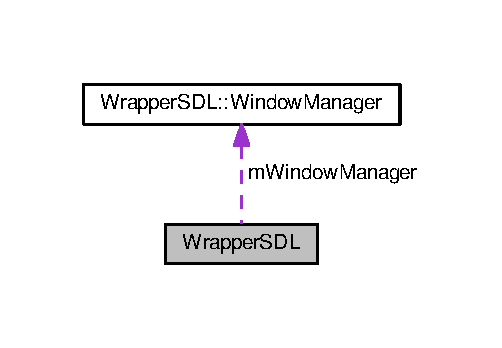
\includegraphics[width=241pt]{struct_wrapper_s_d_l__coll__graph}
\end{center}
\end{figure}
\subsection*{Classes}
\begin{DoxyCompactItemize}
\item 
struct \hyperlink{struct_wrapper_s_d_l_1_1_event_controller}{Event\+Controller}
\item 
struct \hyperlink{struct_wrapper_s_d_l_1_1_window_manager}{Window\+Manager}
\begin{DoxyCompactList}\small\item\em Classe gestionnaire de la fenêtre graphique et du contexte Open\+G\+L. \end{DoxyCompactList}\end{DoxyCompactItemize}
\subsection*{Public Member Functions}
\begin{DoxyCompactItemize}
\item 
void \hyperlink{struct_wrapper_s_d_l_a22e3212f89893ca93010a76df861726b}{Do\+Events\+Loop} (\hyperlink{class_display_manager}{Display\+Manager} $\ast$p\+\_\+\+Params\+Affichage)
\item 
\hyperlink{struct_wrapper_s_d_l_ae0484ea23c2afaae3cdc6ec0a425bdeb}{Wrapper\+S\+D\+L} (int largeur\+Fenetre\+Init, int hauteur\+Fenetre\+Init, const char $\ast$window\+Title)
\item 
void \hyperlink{struct_wrapper_s_d_l_a6731fd378a5431029257edae59bbb6d1}{Init} (\hyperlink{class_display_manager}{Display\+Manager} $\ast$p\+\_\+\+Params\+Affichage)
\end{DoxyCompactItemize}
\subsection*{Public Attributes}
\begin{DoxyCompactItemize}
\item 
\hyperlink{struct_wrapper_s_d_l_1_1_window_manager}{Window\+Manager} \hyperlink{struct_wrapper_s_d_l_a5a50735f512fac9cdae12eb6602589cb}{m\+Window\+Manager}
\end{DoxyCompactItemize}


\subsection{Detailed Description}
Classe Wrapper pour S\+D\+L et assurant les fonctionnalités de la G\+U\+I 

\subsection{Constructor \& Destructor Documentation}
\hypertarget{struct_wrapper_s_d_l_ae0484ea23c2afaae3cdc6ec0a425bdeb}{\index{Wrapper\+S\+D\+L@{Wrapper\+S\+D\+L}!Wrapper\+S\+D\+L@{Wrapper\+S\+D\+L}}
\index{Wrapper\+S\+D\+L@{Wrapper\+S\+D\+L}!Wrapper\+S\+D\+L@{Wrapper\+S\+D\+L}}
\subsubsection[{Wrapper\+S\+D\+L}]{\setlength{\rightskip}{0pt plus 5cm}Wrapper\+S\+D\+L\+::\+Wrapper\+S\+D\+L (
\begin{DoxyParamCaption}
\item[{int}]{largeur\+Fenetre\+Init, }
\item[{int}]{hauteur\+Fenetre\+Init, }
\item[{const char $\ast$}]{window\+Title}
\end{DoxyParamCaption}
)}}\label{struct_wrapper_s_d_l_ae0484ea23c2afaae3cdc6ec0a425bdeb}
Construit la fenêtre graphique au dimensions, ainsi que le contexte Open\+G\+L 

\subsection{Member Function Documentation}
\hypertarget{struct_wrapper_s_d_l_a22e3212f89893ca93010a76df861726b}{\index{Wrapper\+S\+D\+L@{Wrapper\+S\+D\+L}!Do\+Events\+Loop@{Do\+Events\+Loop}}
\index{Do\+Events\+Loop@{Do\+Events\+Loop}!Wrapper\+S\+D\+L@{Wrapper\+S\+D\+L}}
\subsubsection[{Do\+Events\+Loop}]{\setlength{\rightskip}{0pt plus 5cm}void Wrapper\+S\+D\+L\+::\+Do\+Events\+Loop (
\begin{DoxyParamCaption}
\item[{{\bf Display\+Manager} $\ast$}]{p\+\_\+\+Params\+Affichage}
\end{DoxyParamCaption}
)}}\label{struct_wrapper_s_d_l_a22e3212f89893ca93010a76df861726b}
Boucle d'attente des événements \hypertarget{struct_wrapper_s_d_l_a6731fd378a5431029257edae59bbb6d1}{\index{Wrapper\+S\+D\+L@{Wrapper\+S\+D\+L}!Init@{Init}}
\index{Init@{Init}!Wrapper\+S\+D\+L@{Wrapper\+S\+D\+L}}
\subsubsection[{Init}]{\setlength{\rightskip}{0pt plus 5cm}void Wrapper\+S\+D\+L\+::\+Init (
\begin{DoxyParamCaption}
\item[{{\bf Display\+Manager} $\ast$}]{p\+\_\+\+Params\+Affichage}
\end{DoxyParamCaption}
)}}\label{struct_wrapper_s_d_l_a6731fd378a5431029257edae59bbb6d1}
Initialisation de l'instance contenant les données pour implémenter les événements (vue, modèle...) 

\subsection{Member Data Documentation}
\hypertarget{struct_wrapper_s_d_l_a5a50735f512fac9cdae12eb6602589cb}{\index{Wrapper\+S\+D\+L@{Wrapper\+S\+D\+L}!m\+Window\+Manager@{m\+Window\+Manager}}
\index{m\+Window\+Manager@{m\+Window\+Manager}!Wrapper\+S\+D\+L@{Wrapper\+S\+D\+L}}
\subsubsection[{m\+Window\+Manager}]{\setlength{\rightskip}{0pt plus 5cm}{\bf Window\+Manager} Wrapper\+S\+D\+L\+::m\+Window\+Manager}}\label{struct_wrapper_s_d_l_a5a50735f512fac9cdae12eb6602589cb}
Instance de la classe gérant la fenêtre graphique 

The documentation for this struct was generated from the following files\+:\begin{DoxyCompactItemize}
\item 
src/\hyperlink{gui_8hpp}{gui.\+hpp}\item 
src/\hyperlink{gui_8cpp}{gui.\+cpp}\end{DoxyCompactItemize}

\chapter{File Documentation}
\hypertarget{abstract_camera_8cpp}{}\section{src/abstract\+Camera.cpp File Reference}
\label{abstract_camera_8cpp}\index{src/abstract\+Camera.\+cpp@{src/abstract\+Camera.\+cpp}}


Classe abstraite de caméra.  


{\ttfamily \#include \char`\"{}abstract\+Camera.\+hpp\char`\"{}}\\*
{\ttfamily \#include \char`\"{}./camera\+Params/transform.\+hpp\char`\"{}}\\*
Include dependency graph for abstract\+Camera.\+cpp\+:

\hypertarget{abstract_camera_8hpp}{}\section{architecture/abstract\+Camera.hpp File Reference}
\label{abstract_camera_8hpp}\index{architecture/abstract\+Camera.\+hpp@{architecture/abstract\+Camera.\+hpp}}


Classe abstraite de caméra.  


This graph shows which files directly or indirectly include this file\+:
% FIG 0
\subsection*{Classes}
\begin{DoxyCompactItemize}
\item 
class \hyperlink{class_abstract_camera}{Abstract\+Camera}
\begin{DoxyCompactList}\small\item\em Classe de caméra abstraite Classe de caméra abstraite. \end{DoxyCompactList}\end{DoxyCompactItemize}


\subsection{Detailed Description}
Classe abstraite de caméra. 

\begin{DoxyAuthor}{Author}
Pierre Chevalier et Benoît Garçon 
\end{DoxyAuthor}
\begin{DoxyVersion}{Version}
1.\+0 
\end{DoxyVersion}
\begin{DoxyDate}{Date}
Octobre 2016 
\end{DoxyDate}

\hypertarget{abstract_scene_8hpp}{}\section{architecture/abstract\+Scene.hpp File Reference}
\label{abstract_scene_8hpp}\index{architecture/abstract\+Scene.\+hpp@{architecture/abstract\+Scene.\+hpp}}
This graph shows which files directly or indirectly include this file\+:
% FIG 0
\subsection*{Classes}
\begin{DoxyCompactItemize}
\item 
class \hyperlink{class_abstract_scene}{Abstract\+Scene}
\end{DoxyCompactItemize}

\hypertarget{transform_8cpp}{}\section{src/camera\+Params/transform.cpp File Reference}
\label{transform_8cpp}\index{src/camera\+Params/transform.\+cpp@{src/camera\+Params/transform.\+cpp}}


Diverses transformations.  


{\ttfamily \#include \char`\"{}transform.\+hpp\char`\"{}}\\*
Include dependency graph for transform.\+cpp\+:
% FIG 0


\subsection{Detailed Description}
Diverses transformations. 

\begin{DoxyAuthor}{Author}
Pierre Chevalier et Benoît Garçon 
\end{DoxyAuthor}
\begin{DoxyVersion}{Version}
1.\+0 
\end{DoxyVersion}
\begin{DoxyDate}{Date}
Octobre 2016 
\end{DoxyDate}

\hypertarget{transform_8hpp}{}\section{src/camera\+Params/transform.hpp File Reference}
\label{transform_8hpp}\index{src/camera\+Params/transform.\+hpp@{src/camera\+Params/transform.\+hpp}}


Diverses transformations.  


{\ttfamily \#include $<$S\+D\+L2/\+S\+D\+L.\+h$>$}\\*
{\ttfamily \#include $<$S\+D\+L2/\+S\+D\+L\+\_\+opengl.\+h$>$}\\*
{\ttfamily \#include $<$G\+L/glut.\+h$>$}\\*
Include dependency graph for transform.\+hpp\+:
% FIG 0
This graph shows which files directly or indirectly include this file\+:
% FIG 1
\subsection*{Classes}
\begin{DoxyCompactItemize}
\item 
struct \hyperlink{struct_geometric_transform}{Geometric\+Transform}
\end{DoxyCompactItemize}


\subsection{Detailed Description}
Diverses transformations. 

\begin{DoxyAuthor}{Author}
Pierre Chevalier et Benoît Garçon 
\end{DoxyAuthor}
\begin{DoxyVersion}{Version}
1.\+0 
\end{DoxyVersion}
\begin{DoxyDate}{Date}
Octobre 2016 
\end{DoxyDate}

\hypertarget{computed_scene_8cpp}{\section{src/computed\+Scene.cpp File Reference}
\label{computed_scene_8cpp}\index{src/computed\+Scene.\+cpp@{src/computed\+Scene.\+cpp}}
}
{\ttfamily \#include \char`\"{}computed\+Scene.\+hpp\char`\"{}}\\*
Include dependency graph for computed\+Scene.\+cpp\+:
\nopagebreak
\begin{figure}[H]
\begin{center}
\leavevmode
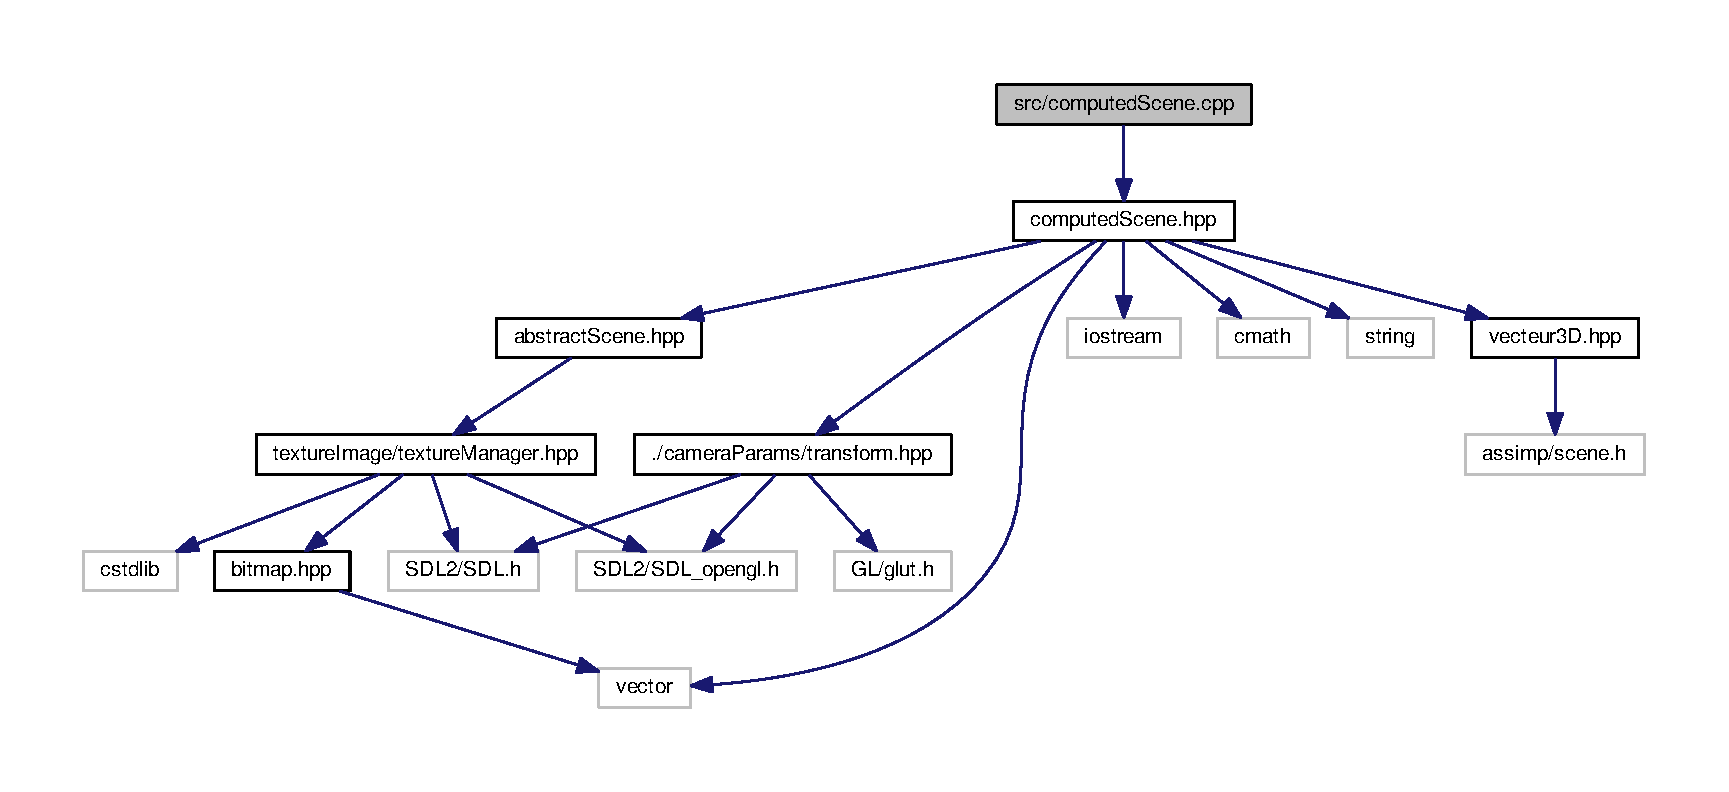
\includegraphics[width=350pt]{computed_scene_8cpp__incl}
\end{center}
\end{figure}

\hypertarget{computed_scene_8hpp}{\section{src/computed\+Scene.hpp File Reference}
\label{computed_scene_8hpp}\index{src/computed\+Scene.\+hpp@{src/computed\+Scene.\+hpp}}
}


\hyperlink{class_scene}{Scene} chargee calculee en temps reel par open\+G\+L.  


{\ttfamily \#include \char`\"{}abstract\+Scene.\+hpp\char`\"{}}\\*
{\ttfamily \#include \char`\"{}./camera\+Params/transform.\+hpp\char`\"{}}\\*
{\ttfamily \#include $<$iostream$>$}\\*
{\ttfamily \#include $<$cmath$>$}\\*
{\ttfamily \#include $<$vector$>$}\\*
{\ttfamily \#include $<$string$>$}\\*
{\ttfamily \#include \char`\"{}vecteur3\+D.\+hpp\char`\"{}}\\*
Include dependency graph for computed\+Scene.\+hpp\+:
\nopagebreak
\begin{figure}[H]
\begin{center}
\leavevmode
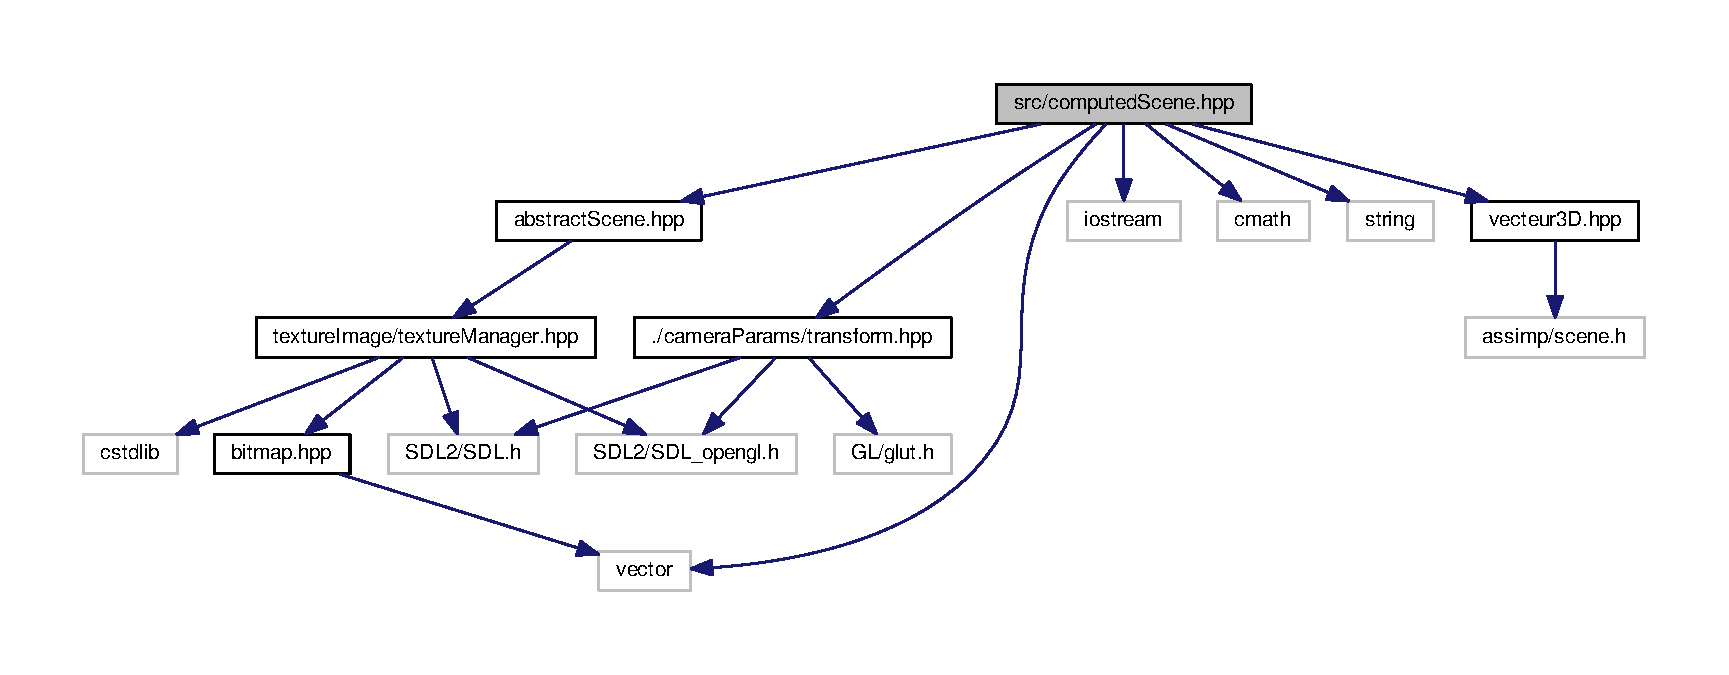
\includegraphics[width=350pt]{computed_scene_8hpp__incl}
\end{center}
\end{figure}
This graph shows which files directly or indirectly include this file\+:
\nopagebreak
\begin{figure}[H]
\begin{center}
\leavevmode
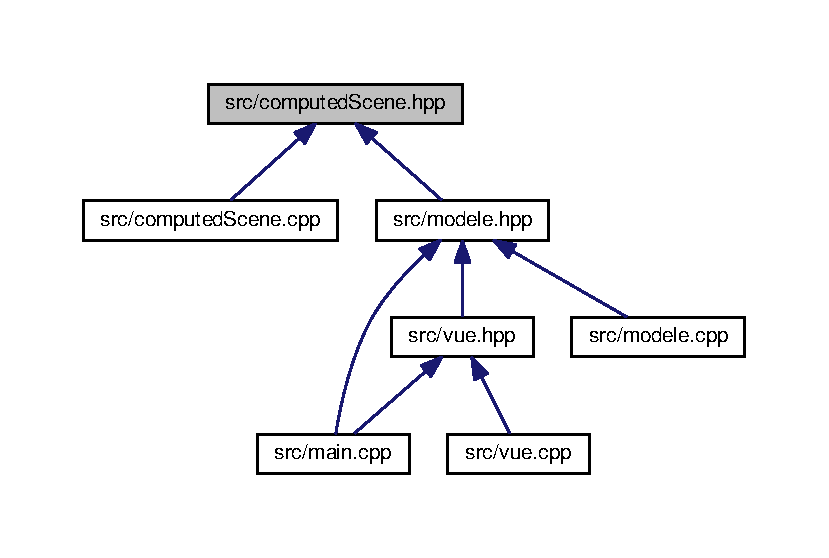
\includegraphics[width=350pt]{computed_scene_8hpp__dep__incl}
\end{center}
\end{figure}
\subsection*{Classes}
\begin{DoxyCompactItemize}
\item 
class \hyperlink{class_teapot}{Teapot}
\item 
class \hyperlink{class_systeme_solaire}{Systeme\+Solaire}
\item 
class \hyperlink{class_voiture}{Voiture}
\item 
class \hyperlink{class_cylindre}{Cylindre}
\end{DoxyCompactItemize}


\subsection{Detailed Description}
\hyperlink{class_scene}{Scene} chargee calculee en temps reel par open\+G\+L. 

\begin{DoxyAuthor}{Author}
Pierre Chevalier et Benoît Garçon 
\end{DoxyAuthor}
\begin{DoxyVersion}{Version}
1.\+0 
\end{DoxyVersion}
\begin{DoxyDate}{Date}
Octobre 2016 
\end{DoxyDate}

\hypertarget{events_handling_8cpp}{\section{src/events\+Handling.cpp File Reference}
\label{events_handling_8cpp}\index{src/events\+Handling.\+cpp@{src/events\+Handling.\+cpp}}
}
{\ttfamily \#include \char`\"{}gui.\+hpp\char`\"{}}\\*
{\ttfamily \#include $<$list$>$}\\*
{\ttfamily \#include $<$algorithm$>$}\\*
{\ttfamily \#include $<$iostream$>$}\\*
Include dependency graph for events\+Handling.\+cpp\+:
\nopagebreak
\begin{figure}[H]
\begin{center}
\leavevmode
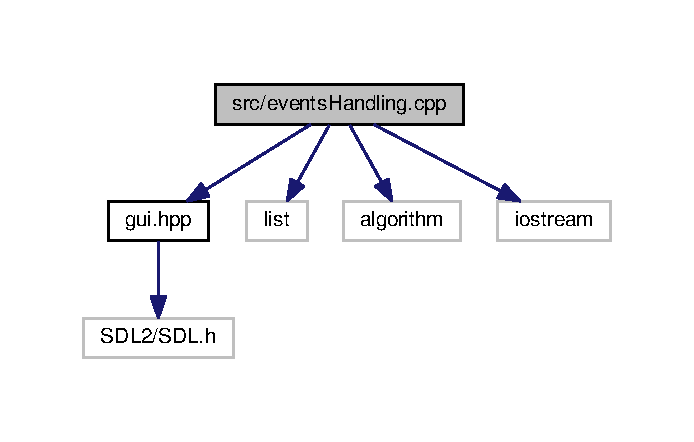
\includegraphics[width=333pt]{events_handling_8cpp__incl}
\end{center}
\end{figure}
This graph shows which files directly or indirectly include this file\+:
\nopagebreak
\begin{figure}[H]
\begin{center}
\leavevmode
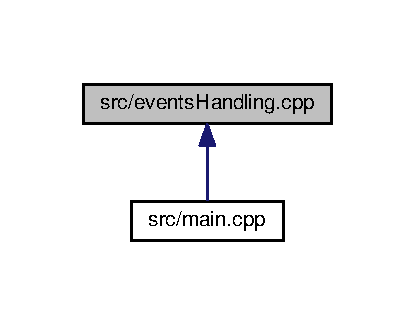
\includegraphics[width=199pt]{events_handling_8cpp__dep__incl}
\end{center}
\end{figure}
\subsection*{Macros}
\begin{DoxyCompactItemize}
\item 
\#define \hyperlink{events_handling_8cpp_aee5cc60cf83fe16165b0a0a0158cce48}{V\+I\+T\+E\+S\+S\+E\+K\+E\+Y}~10
\item 
\#define \hyperlink{events_handling_8cpp_a89a95330796f9b63426f99f954d2f959}{V\+I\+T\+E\+S\+S\+E\+M\+O\+U}~100
\item 
\#define \hyperlink{events_handling_8cpp_a86cdb1366106e812b372a5d1cd16cebf}{V\+I\+T\+E\+S\+S\+E\+R\+O\+T}~5
\end{DoxyCompactItemize}
\subsection*{Functions}
\begin{DoxyCompactItemize}
\item 
bool \hyperlink{events_handling_8cpp_a097d525e851b25aa1aee029411df940b}{manage\+Pressed\+Keys} (std\+::list$<$ int $>$ keys, \hyperlink{class_display_manager}{Display\+Manager} $\ast$p\+\_\+\+Params\+Affichage)
\begin{DoxyCompactList}\small\item\em Gestion d'un événement S\+D\+L extrait de la file. \end{DoxyCompactList}\item 
void \hyperlink{events_handling_8cpp_a1fc0df626da9b5be5381611bff4536de}{manage\+Cam\+Move} (\hyperlink{class_display_manager}{Display\+Manager} $\ast$p\+\_\+\+Params\+Affichage)
\begin{DoxyCompactList}\small\item\em Gère le déplacement de la caméra. \end{DoxyCompactList}\item 
void \hyperlink{events_handling_8cpp_a1627593ba47af47c7f1bc466937cd58e}{manage\+Cam\+Angle} (\hyperlink{class_display_manager}{Display\+Manager} $\ast$p\+\_\+\+Params\+Affichage)
\begin{DoxyCompactList}\small\item\em Gère l'orientation de la caméra. \end{DoxyCompactList}\end{DoxyCompactItemize}


\subsection{Macro Definition Documentation}
\hypertarget{events_handling_8cpp_aee5cc60cf83fe16165b0a0a0158cce48}{\index{events\+Handling.\+cpp@{events\+Handling.\+cpp}!V\+I\+T\+E\+S\+S\+E\+K\+E\+Y@{V\+I\+T\+E\+S\+S\+E\+K\+E\+Y}}
\index{V\+I\+T\+E\+S\+S\+E\+K\+E\+Y@{V\+I\+T\+E\+S\+S\+E\+K\+E\+Y}!events\+Handling.\+cpp@{events\+Handling.\+cpp}}
\subsubsection[{V\+I\+T\+E\+S\+S\+E\+K\+E\+Y}]{\setlength{\rightskip}{0pt plus 5cm}\#define V\+I\+T\+E\+S\+S\+E\+K\+E\+Y~10}}\label{events_handling_8cpp_aee5cc60cf83fe16165b0a0a0158cce48}
\hypertarget{events_handling_8cpp_a89a95330796f9b63426f99f954d2f959}{\index{events\+Handling.\+cpp@{events\+Handling.\+cpp}!V\+I\+T\+E\+S\+S\+E\+M\+O\+U@{V\+I\+T\+E\+S\+S\+E\+M\+O\+U}}
\index{V\+I\+T\+E\+S\+S\+E\+M\+O\+U@{V\+I\+T\+E\+S\+S\+E\+M\+O\+U}!events\+Handling.\+cpp@{events\+Handling.\+cpp}}
\subsubsection[{V\+I\+T\+E\+S\+S\+E\+M\+O\+U}]{\setlength{\rightskip}{0pt plus 5cm}\#define V\+I\+T\+E\+S\+S\+E\+M\+O\+U~100}}\label{events_handling_8cpp_a89a95330796f9b63426f99f954d2f959}
\hypertarget{events_handling_8cpp_a86cdb1366106e812b372a5d1cd16cebf}{\index{events\+Handling.\+cpp@{events\+Handling.\+cpp}!V\+I\+T\+E\+S\+S\+E\+R\+O\+T@{V\+I\+T\+E\+S\+S\+E\+R\+O\+T}}
\index{V\+I\+T\+E\+S\+S\+E\+R\+O\+T@{V\+I\+T\+E\+S\+S\+E\+R\+O\+T}!events\+Handling.\+cpp@{events\+Handling.\+cpp}}
\subsubsection[{V\+I\+T\+E\+S\+S\+E\+R\+O\+T}]{\setlength{\rightskip}{0pt plus 5cm}\#define V\+I\+T\+E\+S\+S\+E\+R\+O\+T~5}}\label{events_handling_8cpp_a86cdb1366106e812b372a5d1cd16cebf}


\subsection{Function Documentation}
\hypertarget{events_handling_8cpp_a1627593ba47af47c7f1bc466937cd58e}{\index{events\+Handling.\+cpp@{events\+Handling.\+cpp}!manage\+Cam\+Angle@{manage\+Cam\+Angle}}
\index{manage\+Cam\+Angle@{manage\+Cam\+Angle}!events\+Handling.\+cpp@{events\+Handling.\+cpp}}
\subsubsection[{manage\+Cam\+Angle}]{\setlength{\rightskip}{0pt plus 5cm}void manage\+Cam\+Angle (
\begin{DoxyParamCaption}
\item[{{\bf Display\+Manager} $\ast$}]{p\+\_\+\+Params\+Affichage}
\end{DoxyParamCaption}
)}}\label{events_handling_8cpp_a1627593ba47af47c7f1bc466937cd58e}


Gère l'orientation de la caméra. 


\begin{DoxyParams}{Parameters}
{\em Le} & display manager \\
\hline
\end{DoxyParams}
\hypertarget{events_handling_8cpp_a1fc0df626da9b5be5381611bff4536de}{\index{events\+Handling.\+cpp@{events\+Handling.\+cpp}!manage\+Cam\+Move@{manage\+Cam\+Move}}
\index{manage\+Cam\+Move@{manage\+Cam\+Move}!events\+Handling.\+cpp@{events\+Handling.\+cpp}}
\subsubsection[{manage\+Cam\+Move}]{\setlength{\rightskip}{0pt plus 5cm}void manage\+Cam\+Move (
\begin{DoxyParamCaption}
\item[{{\bf Display\+Manager} $\ast$}]{p\+\_\+\+Params\+Affichage}
\end{DoxyParamCaption}
)}}\label{events_handling_8cpp_a1fc0df626da9b5be5381611bff4536de}


Gère le déplacement de la caméra. 


\begin{DoxyParams}{Parameters}
{\em Le} & display manager \\
\hline
\end{DoxyParams}
\hypertarget{events_handling_8cpp_a097d525e851b25aa1aee029411df940b}{\index{events\+Handling.\+cpp@{events\+Handling.\+cpp}!manage\+Pressed\+Keys@{manage\+Pressed\+Keys}}
\index{manage\+Pressed\+Keys@{manage\+Pressed\+Keys}!events\+Handling.\+cpp@{events\+Handling.\+cpp}}
\subsubsection[{manage\+Pressed\+Keys}]{\setlength{\rightskip}{0pt plus 5cm}bool manage\+Pressed\+Keys (
\begin{DoxyParamCaption}
\item[{std\+::list$<$ int $>$}]{keys, }
\item[{{\bf Display\+Manager} $\ast$}]{p\+\_\+\+Params\+Affichage}
\end{DoxyParamCaption}
)}}\label{events_handling_8cpp_a097d525e851b25aa1aee029411df940b}


Gestion d'un événement S\+D\+L extrait de la file. 


\begin{DoxyParams}{Parameters}
{\em p\+\_\+evenement} & données de l'événement \\
\hline
{\em window} & Fenêtre S\+D\+L (pour gérer les S\+D\+L\+\_\+\+W\+I\+N\+D\+O\+W\+E\+V\+E\+N\+T) \\
\hline
{\em p\+\_\+\+Params\+Affichage} & instance de la classe Vue \\
\hline
\end{DoxyParams}
\begin{DoxyReturn}{Returns}
true si l'événement est S\+D\+L\+\_\+\+Q\+U\+I\+T (fermeture de la fenêtre) 
\end{DoxyReturn}

\hypertarget{frames_8cpp}{}\section{architecture/frames.cpp File Reference}
\label{frames_8cpp}\index{architecture/frames.\+cpp@{architecture/frames.\+cpp}}
{\ttfamily \#include \char`\"{}frames.\+hpp\char`\"{}}\\*
{\ttfamily \#include $<$cstdio$>$}\\*
{\ttfamily \#include $<$cstring$>$}\\*
{\ttfamily \#include $<$S\+D\+L2/\+S\+D\+L.\+h$>$}\\*
Include dependency graph for frames.\+cpp\+:
% FIG 0

\hypertarget{frames_8hpp}{\section{src/frames.hpp File Reference}
\label{frames_8hpp}\index{src/frames.\+hpp@{src/frames.\+hpp}}
}


Classe de gestion des frames.  


This graph shows which files directly or indirectly include this file\+:
\nopagebreak
\begin{figure}[H]
\begin{center}
\leavevmode
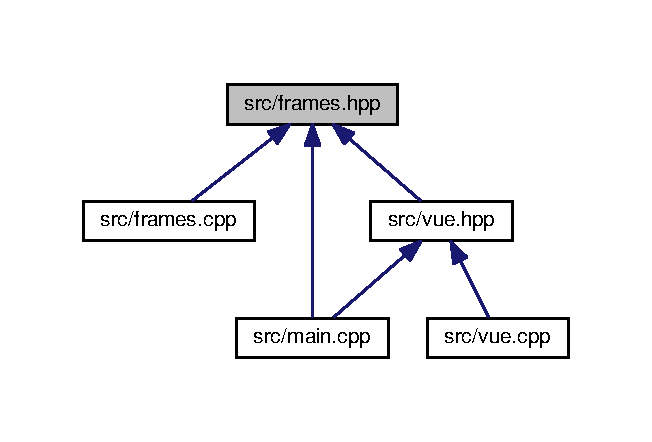
\includegraphics[width=313pt]{frames_8hpp__dep__incl}
\end{center}
\end{figure}
\subsection*{Classes}
\begin{DoxyCompactItemize}
\item 
class \hyperlink{class_frames_data}{Frames\+Data}
\end{DoxyCompactItemize}


\subsection{Detailed Description}
Classe de gestion des frames. 

\begin{DoxyAuthor}{Author}
Pierre Chevalier et Benoît Garçon 
\end{DoxyAuthor}
\begin{DoxyVersion}{Version}
1.\+0 
\end{DoxyVersion}
\begin{DoxyDate}{Date}
Octobre 2016 
\end{DoxyDate}

\hypertarget{gui_8cpp}{\section{src/gui.cpp File Reference}
\label{gui_8cpp}\index{src/gui.\+cpp@{src/gui.\+cpp}}
}


Wrapper S\+D\+L.  


{\ttfamily \#include \char`\"{}gui.\+hpp\char`\"{}}\\*
Include dependency graph for gui.\+cpp\+:
\nopagebreak
\begin{figure}[H]
\begin{center}
\leavevmode
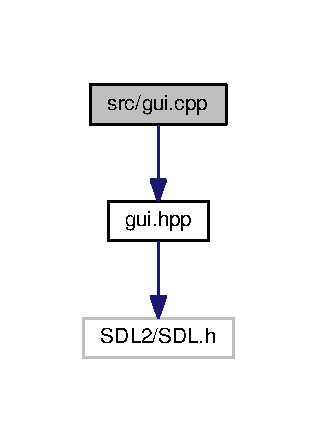
\includegraphics[width=152pt]{gui_8cpp__incl}
\end{center}
\end{figure}


\subsection{Detailed Description}
Wrapper S\+D\+L. 

\begin{DoxyAuthor}{Author}
Pierre Chevalier et Benoît Garçon 
\end{DoxyAuthor}
\begin{DoxyVersion}{Version}
1.\+0 
\end{DoxyVersion}
\begin{DoxyDate}{Date}
Octobre 2016 
\end{DoxyDate}

\hypertarget{gui_8hpp}{}\section{architecture/gui.hpp File Reference}
\label{gui_8hpp}\index{architecture/gui.\+hpp@{architecture/gui.\+hpp}}
{\ttfamily \#include $<$S\+D\+L2/\+S\+D\+L.\+h$>$}\\*
Include dependency graph for gui.\+hpp\+:
% FIG 0
This graph shows which files directly or indirectly include this file\+:
% FIG 1
\subsection*{Classes}
\begin{DoxyCompactItemize}
\item 
struct \hyperlink{struct_wrapper_s_d_l}{Wrapper\+S\+DL}
\item 
struct \hyperlink{struct_wrapper_s_d_l_1_1_event_controller}{Wrapper\+S\+D\+L\+::\+Event\+Controller}
\item 
struct \hyperlink{struct_wrapper_s_d_l_1_1_window_manager}{Wrapper\+S\+D\+L\+::\+Window\+Manager}
\begin{DoxyCompactList}\small\item\em Classe gestionnaire de la fenêtre graphique et du contexte Open\+GL. \end{DoxyCompactList}\end{DoxyCompactItemize}

\hypertarget{look_at_camera_8cpp}{}\section{src/look\+At\+Camera.cpp File Reference}
\label{look_at_camera_8cpp}\index{src/look\+At\+Camera.\+cpp@{src/look\+At\+Camera.\+cpp}}


Classe de caméra utilisant glu\+Look\+At.  


{\ttfamily \#include \char`\"{}look\+At\+Camera.\+hpp\char`\"{}}\\*
{\ttfamily \#include \char`\"{}./camera\+Params/transform.\+hpp\char`\"{}}\\*
{\ttfamily \#include $<$iostream$>$}\\*
Include dependency graph for look\+At\+Camera.\+cpp\+:
% FIG 0


\subsection{Detailed Description}
Classe de caméra utilisant glu\+Look\+At. 

\begin{DoxyAuthor}{Author}
Pierre Chevalier et Benoît Garçon 
\end{DoxyAuthor}
\begin{DoxyVersion}{Version}
1.\+0 
\end{DoxyVersion}
\begin{DoxyDate}{Date}
Octobre 2016 
\end{DoxyDate}

\hypertarget{look_at_camera_8hpp}{}\section{src/look\+At\+Camera.hpp File Reference}
\label{look_at_camera_8hpp}\index{src/look\+At\+Camera.\+hpp@{src/look\+At\+Camera.\+hpp}}


Classe de caméra utilisant glu\+Look\+At.  


{\ttfamily \#include \char`\"{}abstract\+Camera.\+hpp\char`\"{}}\\*
Include dependency graph for look\+At\+Camera.\+hpp\+:
% FIG 0
This graph shows which files directly or indirectly include this file\+:
% FIG 1
\subsection*{Classes}
\begin{DoxyCompactItemize}
\item 
class \hyperlink{class_look_at_camera}{Look\+At\+Camera}
\begin{DoxyCompactList}\small\item\em Classe de caméra utilisant glu\+Look\+At Classe de caméra utilisant glu\+Look\+At et héritant de \hyperlink{class_abstract_camera}{Abstract\+Camera}. \end{DoxyCompactList}\end{DoxyCompactItemize}


\subsection{Detailed Description}
Classe de caméra utilisant glu\+Look\+At. 

\begin{DoxyAuthor}{Author}
Pierre Chevalier et Benoît Garçon 
\end{DoxyAuthor}
\begin{DoxyVersion}{Version}
1.\+0 
\end{DoxyVersion}
\begin{DoxyDate}{Date}
Octobre 2016 
\end{DoxyDate}

\hypertarget{maillage_8cpp}{\section{src/maillage.cpp File Reference}
\label{maillage_8cpp}\index{src/maillage.\+cpp@{src/maillage.\+cpp}}
}


Classe de maillage.  


{\ttfamily \#include \char`\"{}maillage.\+hpp\char`\"{}}\\*
Include dependency graph for maillage.\+cpp\+:
\nopagebreak
\begin{figure}[H]
\begin{center}
\leavevmode
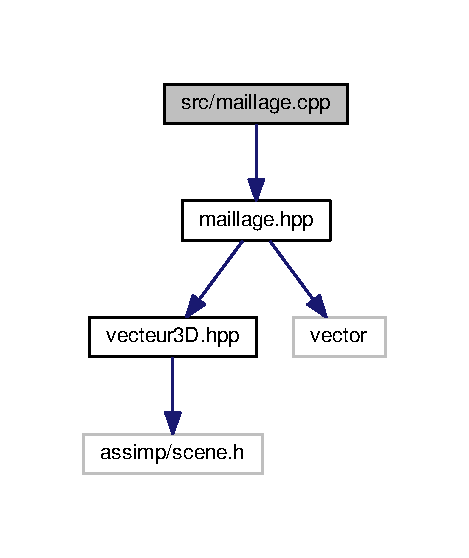
\includegraphics[width=225pt]{maillage_8cpp__incl}
\end{center}
\end{figure}


\subsection{Detailed Description}
Classe de maillage. 

\begin{DoxyAuthor}{Author}
Pierre Chevalier et Benoît Garçon 
\end{DoxyAuthor}
\begin{DoxyVersion}{Version}
1.\+0 
\end{DoxyVersion}
\begin{DoxyDate}{Date}
Octobre 2016 
\end{DoxyDate}

\hypertarget{maillage_8hpp}{\section{src/maillage.hpp File Reference}
\label{maillage_8hpp}\index{src/maillage.\+hpp@{src/maillage.\+hpp}}
}


Classe de maillage.  


{\ttfamily \#include \char`\"{}vecteur3\+D.\+hpp\char`\"{}}\\*
{\ttfamily \#include $<$vector$>$}\\*
Include dependency graph for maillage.\+hpp\+:
\nopagebreak
\begin{figure}[H]
\begin{center}
\leavevmode
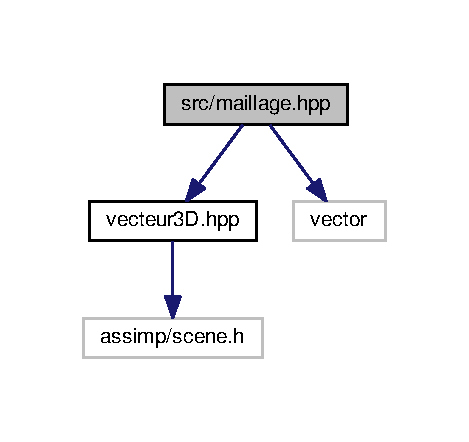
\includegraphics[width=225pt]{maillage_8hpp__incl}
\end{center}
\end{figure}
This graph shows which files directly or indirectly include this file\+:
\nopagebreak
\begin{figure}[H]
\begin{center}
\leavevmode
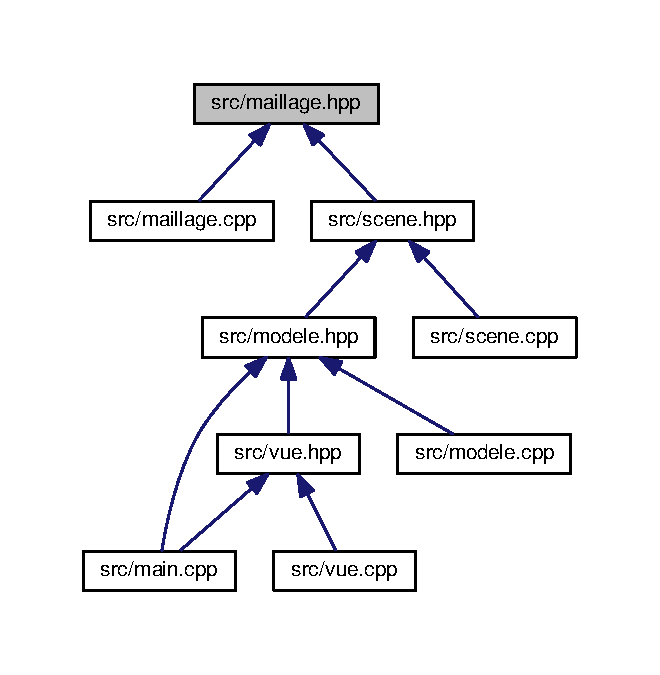
\includegraphics[width=317pt]{maillage_8hpp__dep__incl}
\end{center}
\end{figure}
\subsection*{Classes}
\begin{DoxyCompactItemize}
\item 
class \hyperlink{class_maillage}{Maillage}
\end{DoxyCompactItemize}


\subsection{Detailed Description}
Classe de maillage. 

\begin{DoxyAuthor}{Author}
Pierre Chevalier et Benoît Garçon 
\end{DoxyAuthor}
\begin{DoxyVersion}{Version}
1.\+0 
\end{DoxyVersion}
\begin{DoxyDate}{Date}
Octobre 2016 
\end{DoxyDate}

\hypertarget{main_8cpp}{}\section{architecture/main.cpp File Reference}
\label{main_8cpp}\index{architecture/main.\+cpp@{architecture/main.\+cpp}}
{\ttfamily \#include $<$stdlib.\+h$>$}\\*
{\ttfamily \#include $<$stdio.\+h$>$}\\*
{\ttfamily \#include $<$S\+D\+L2/\+S\+D\+L.\+h$>$}\\*
{\ttfamily \#include $<$S\+D\+L2/\+S\+D\+L\+\_\+opengl.\+h$>$}\\*
{\ttfamily \#include $<$G\+L/glut.\+h$>$}\\*
{\ttfamily \#include \char`\"{}frames.\+hpp\char`\"{}}\\*
{\ttfamily \#include \char`\"{}modele.\+hpp\char`\"{}}\\*
{\ttfamily \#include \char`\"{}../camera\+Params/transform.\+hpp\char`\"{}}\\*
{\ttfamily \#include \char`\"{}vue.\+hpp\char`\"{}}\\*
{\ttfamily \#include \char`\"{}mouse.\+hpp\char`\"{}}\\*
{\ttfamily \#include \char`\"{}gui.\+hpp\char`\"{}}\\*
{\ttfamily \#include \char`\"{}events\+Handling.\+cpp\char`\"{}}\\*
Include dependency graph for main.\+cpp\+:
% FIG 0
\subsection*{Classes}
\begin{DoxyCompactItemize}
\item 
struct \hyperlink{struct_main_application}{Main\+Application}
\end{DoxyCompactItemize}
\subsection*{Functions}
\begin{DoxyCompactItemize}
\item 
int \hyperlink{main_8cpp_a3c04138a5bfe5d72780bb7e82a18e627}{main} (int argc, char $\ast$$\ast$argv)
\end{DoxyCompactItemize}


\subsection{Function Documentation}
\index{main.\+cpp@{main.\+cpp}!main@{main}}
\index{main@{main}!main.\+cpp@{main.\+cpp}}
\subsubsection[{\texorpdfstring{main(int argc, char $\ast$$\ast$argv)}{main(int argc, char **argv)}}]{\setlength{\rightskip}{0pt plus 5cm}int main (
\begin{DoxyParamCaption}
\item[{int}]{argc, }
\item[{char $\ast$$\ast$}]{argv}
\end{DoxyParamCaption}
)}\hypertarget{main_8cpp_a3c04138a5bfe5d72780bb7e82a18e627}{}\label{main_8cpp_a3c04138a5bfe5d72780bb7e82a18e627}

\hypertarget{modele_8cpp}{\section{src/modele.cpp File Reference}
\label{modele_8cpp}\index{src/modele.\+cpp@{src/modele.\+cpp}}
}


Classe du modèle de M\+V\+C.  


{\ttfamily \#include \char`\"{}modele.\+hpp\char`\"{}}\\*
Include dependency graph for modele.\+cpp\+:
\nopagebreak
\begin{figure}[H]
\begin{center}
\leavevmode
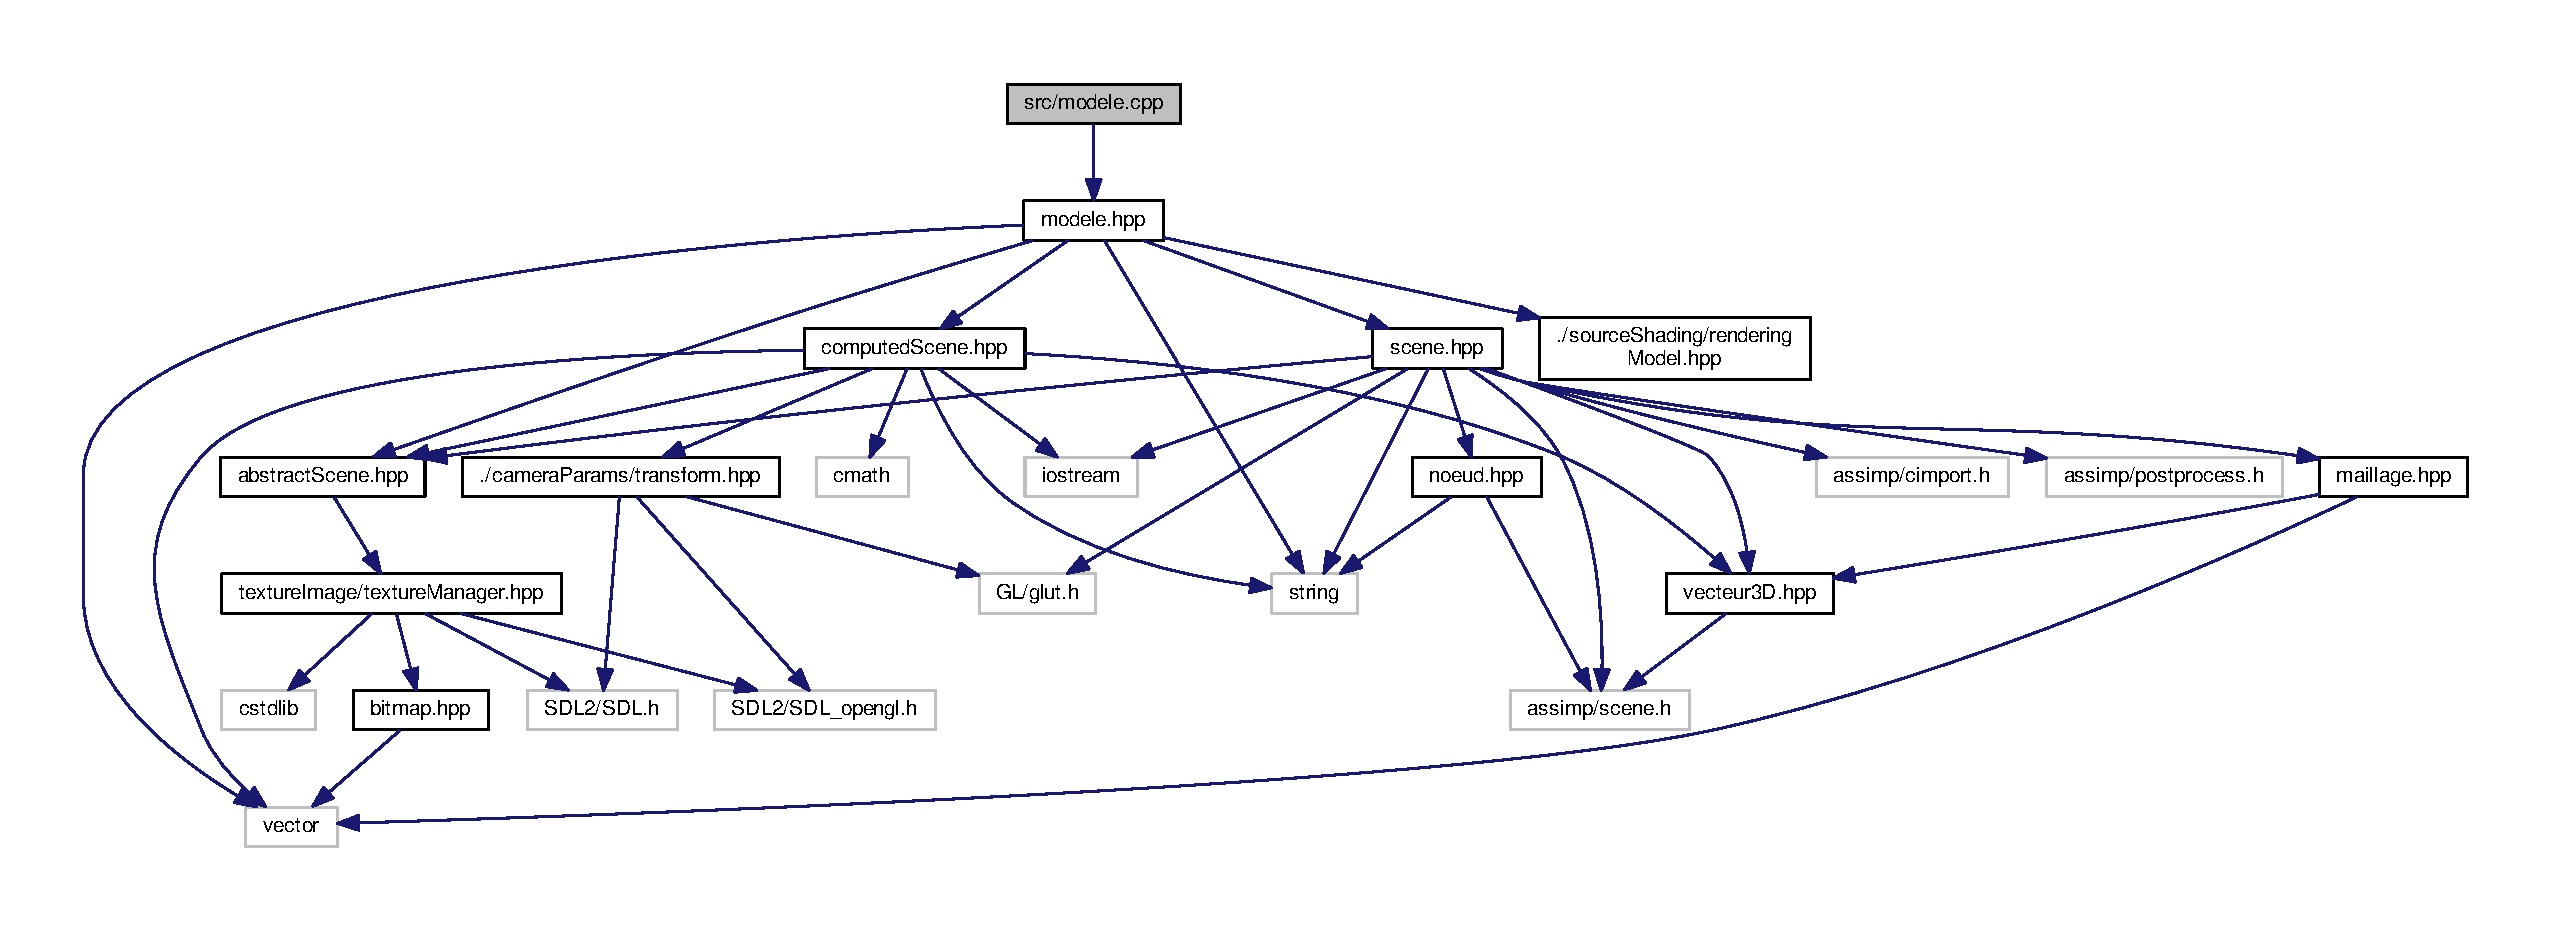
\includegraphics[width=350pt]{modele_8cpp__incl}
\end{center}
\end{figure}


\subsection{Detailed Description}
Classe du modèle de M\+V\+C. 

\begin{DoxyAuthor}{Author}
Pierre Chevalier et Benoît Garçon 
\end{DoxyAuthor}
\begin{DoxyVersion}{Version}
1.\+0 
\end{DoxyVersion}
\begin{DoxyDate}{Date}
Octobre 2016 
\end{DoxyDate}

\hypertarget{modele_8hpp}{}\section{architecture/modele.hpp File Reference}
\label{modele_8hpp}\index{architecture/modele.\+hpp@{architecture/modele.\+hpp}}
{\ttfamily \#include $<$string$>$}\\*
{\ttfamily \#include $<$vector$>$}\\*
{\ttfamily \#include \char`\"{}scene.\+hpp\char`\"{}}\\*
{\ttfamily \#include \char`\"{}abstract\+Scene.\+hpp\char`\"{}}\\*
{\ttfamily \#include \char`\"{}computed\+Scene.\+hpp\char`\"{}}\\*
{\ttfamily \#include \char`\"{}../source\+Shading/rendering\+Model.\+hpp\char`\"{}}\\*
Include dependency graph for modele.\+hpp\+:
% FIG 0
This graph shows which files directly or indirectly include this file\+:
% FIG 1
\subsection*{Classes}
\begin{DoxyCompactItemize}
\item 
class \hyperlink{class_modele}{Modele}
\end{DoxyCompactItemize}

\hypertarget{mouse_8cpp}{\section{src/mouse.cpp File Reference}
\label{mouse_8cpp}\index{src/mouse.\+cpp@{src/mouse.\+cpp}}
}


Classe de gestion de la souris.  


{\ttfamily \#include \char`\"{}mouse.\+hpp\char`\"{}}\\*
Include dependency graph for mouse.\+cpp\+:
\nopagebreak
\begin{figure}[H]
\begin{center}
\leavevmode
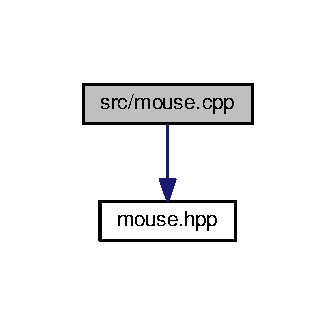
\includegraphics[width=161pt]{mouse_8cpp__incl}
\end{center}
\end{figure}


\subsection{Detailed Description}
Classe de gestion de la souris. 

\begin{DoxyAuthor}{Author}
Pierre Chevalier et Benoît Garçon 
\end{DoxyAuthor}
\begin{DoxyVersion}{Version}
1.\+0 
\end{DoxyVersion}
\begin{DoxyDate}{Date}
Octobre 2016 
\end{DoxyDate}

\hypertarget{mouse_8hpp}{}\section{src/mouse.hpp File Reference}
\label{mouse_8hpp}\index{src/mouse.\+hpp@{src/mouse.\+hpp}}


Classe de gestion de la souris.  


This graph shows which files directly or indirectly include this file\+:
% FIG 0
\subsection*{Classes}
\begin{DoxyCompactItemize}
\item 
class \hyperlink{class_mouse_data}{Mouse\+Data}
\begin{DoxyCompactList}\small\item\em Modèle pour la souris (interaction utilisateur) Paramètres concernant la souris (état, vitesse, etc) \end{DoxyCompactList}\end{DoxyCompactItemize}


\subsection{Detailed Description}
Classe de gestion de la souris. 

\begin{DoxyAuthor}{Author}
Pierre Chevalier et Benoît Garçon 
\end{DoxyAuthor}
\begin{DoxyVersion}{Version}
1.\+0 
\end{DoxyVersion}
\begin{DoxyDate}{Date}
Octobre 2016 
\end{DoxyDate}

\hypertarget{noeud_8cpp}{}\section{src/noeud.cpp File Reference}
\label{noeud_8cpp}\index{src/noeud.\+cpp@{src/noeud.\+cpp}}
{\ttfamily \#include \char`\"{}noeud.\+hpp\char`\"{}}\\*
Include dependency graph for noeud.\+cpp\+:
% FIG 0

\hypertarget{noeud_8hpp}{}\section{architecture/noeud.hpp File Reference}
\label{noeud_8hpp}\index{architecture/noeud.\+hpp@{architecture/noeud.\+hpp}}
{\ttfamily \#include $<$assimp/scene.\+h$>$}\\*
{\ttfamily \#include $<$string$>$}\\*
Include dependency graph for noeud.\+hpp\+:
% FIG 0
This graph shows which files directly or indirectly include this file\+:
% FIG 1
\subsection*{Classes}
\begin{DoxyCompactItemize}
\item 
class \hyperlink{class_noeud}{Noeud}
\end{DoxyCompactItemize}

\hypertarget{scene_8cpp}{}\section{src/scene.cpp File Reference}
\label{scene_8cpp}\index{src/scene.\+cpp@{src/scene.\+cpp}}
{\ttfamily \#include \char`\"{}scene.\+hpp\char`\"{}}\\*
Include dependency graph for scene.\+cpp\+:
% FIG 0

\hypertarget{scene_8hpp}{\section{src/scene.hpp File Reference}
\label{scene_8hpp}\index{src/scene.\+hpp@{src/scene.\+hpp}}
}


\hyperlink{class_scene}{Scene} chargee par fichier.  


{\ttfamily \#include $<$string$>$}\\*
{\ttfamily \#include $<$iostream$>$}\\*
{\ttfamily \#include $<$assimp/cimport.\+h$>$}\\*
{\ttfamily \#include $<$assimp/scene.\+h$>$}\\*
{\ttfamily \#include $<$assimp/postprocess.\+h$>$}\\*
{\ttfamily \#include $<$G\+L/glut.\+h$>$}\\*
{\ttfamily \#include \char`\"{}abstract\+Scene.\+hpp\char`\"{}}\\*
{\ttfamily \#include \char`\"{}vecteur3\+D.\+hpp\char`\"{}}\\*
{\ttfamily \#include \char`\"{}noeud.\+hpp\char`\"{}}\\*
{\ttfamily \#include \char`\"{}maillage.\+hpp\char`\"{}}\\*
Include dependency graph for scene.\+hpp\+:
\nopagebreak
\begin{figure}[H]
\begin{center}
\leavevmode
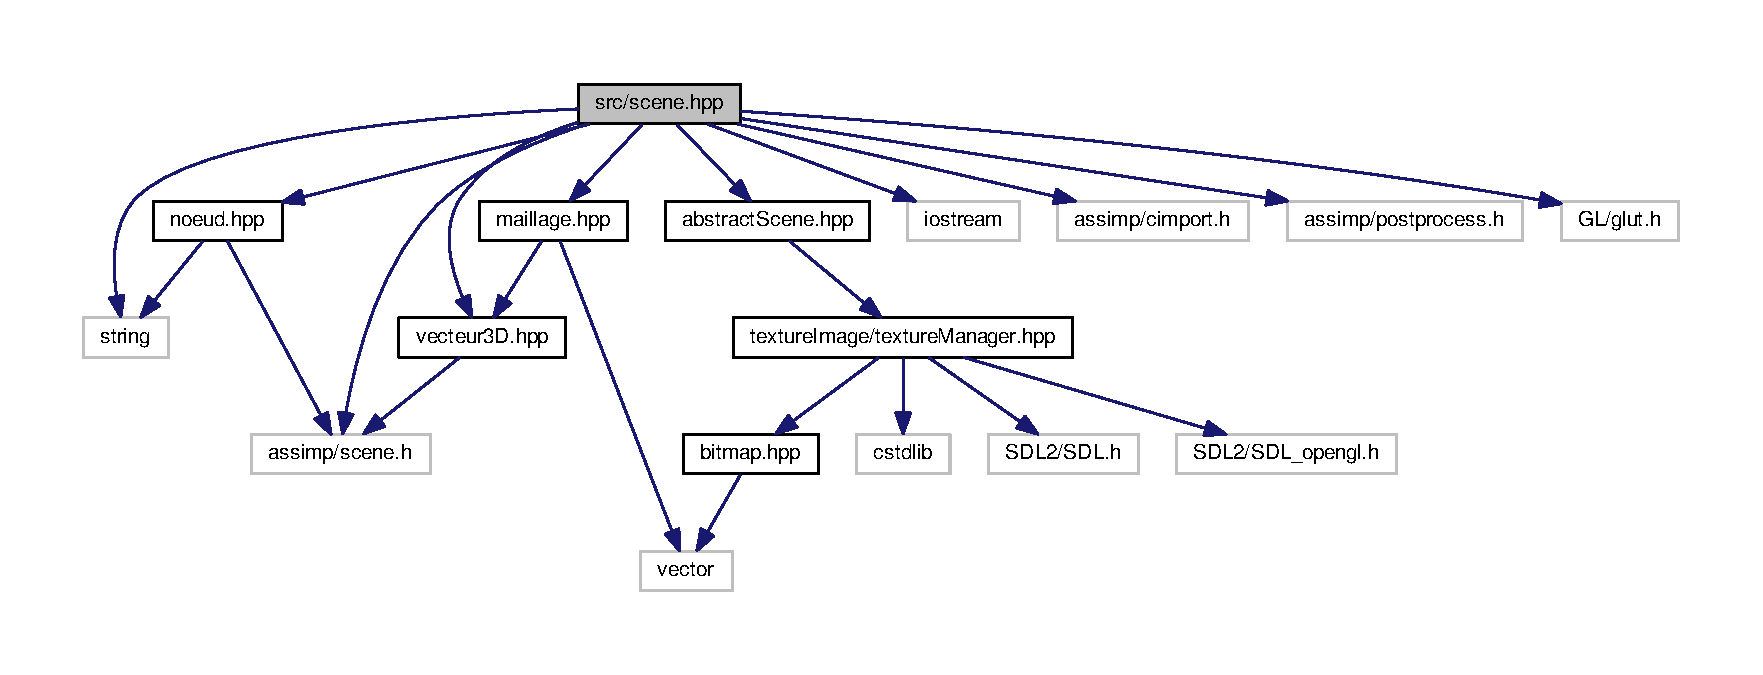
\includegraphics[width=350pt]{scene_8hpp__incl}
\end{center}
\end{figure}
This graph shows which files directly or indirectly include this file\+:
\nopagebreak
\begin{figure}[H]
\begin{center}
\leavevmode
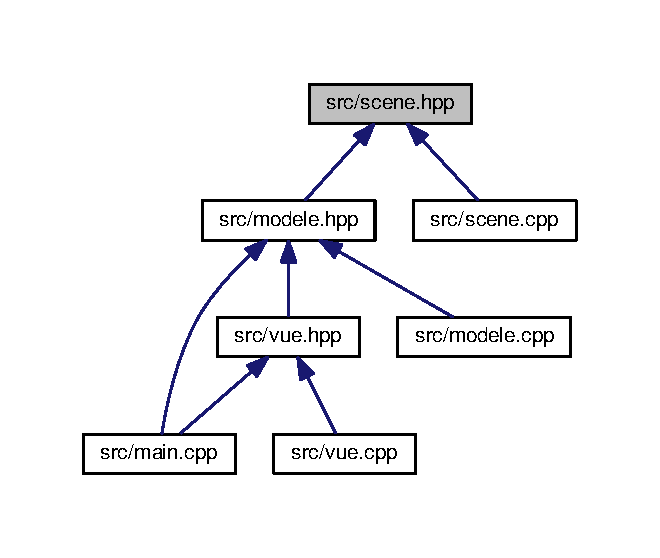
\includegraphics[width=317pt]{scene_8hpp__dep__incl}
\end{center}
\end{figure}
\subsection*{Classes}
\begin{DoxyCompactItemize}
\item 
class \hyperlink{class_scene}{Scene}
\end{DoxyCompactItemize}
\subsection*{Macros}
\begin{DoxyCompactItemize}
\item 
\#define \hyperlink{scene_8hpp_ae19f66e94255e323687e3dcdd5362125}{aisgl\+\_\+min}(x, y)~(x$<$y?x\+:y)
\item 
\#define \hyperlink{scene_8hpp_a5d7d752ed7ce95f82f595ac2e5e300aa}{aisgl\+\_\+max}(x, y)~(y$>$x?y\+:x)
\end{DoxyCompactItemize}


\subsection{Detailed Description}
\hyperlink{class_scene}{Scene} chargee par fichier. 

\begin{DoxyAuthor}{Author}
Pierre Chevalier et Benoît Garçon 
\end{DoxyAuthor}
\begin{DoxyVersion}{Version}
1.\+0 
\end{DoxyVersion}
\begin{DoxyDate}{Date}
Octobre 2016 
\end{DoxyDate}


\subsection{Macro Definition Documentation}
\hypertarget{scene_8hpp_a5d7d752ed7ce95f82f595ac2e5e300aa}{\index{scene.\+hpp@{scene.\+hpp}!aisgl\+\_\+max@{aisgl\+\_\+max}}
\index{aisgl\+\_\+max@{aisgl\+\_\+max}!scene.\+hpp@{scene.\+hpp}}
\subsubsection[{aisgl\+\_\+max}]{\setlength{\rightskip}{0pt plus 5cm}\#define aisgl\+\_\+max(
\begin{DoxyParamCaption}
\item[{}]{x, }
\item[{}]{y}
\end{DoxyParamCaption}
)~(y$>$x?y\+:x)}}\label{scene_8hpp_a5d7d752ed7ce95f82f595ac2e5e300aa}
\hypertarget{scene_8hpp_ae19f66e94255e323687e3dcdd5362125}{\index{scene.\+hpp@{scene.\+hpp}!aisgl\+\_\+min@{aisgl\+\_\+min}}
\index{aisgl\+\_\+min@{aisgl\+\_\+min}!scene.\+hpp@{scene.\+hpp}}
\subsubsection[{aisgl\+\_\+min}]{\setlength{\rightskip}{0pt plus 5cm}\#define aisgl\+\_\+min(
\begin{DoxyParamCaption}
\item[{}]{x, }
\item[{}]{y}
\end{DoxyParamCaption}
)~(x$<$y?x\+:y)}}\label{scene_8hpp_ae19f66e94255e323687e3dcdd5362125}

\hypertarget{light_8hpp}{}\section{src/source\+Shading/light.hpp File Reference}
\label{light_8hpp}\index{src/source\+Shading/light.\+hpp@{src/source\+Shading/light.\+hpp}}


Classes de lumière.  


{\ttfamily \#include $<$vector$>$}\\*
{\ttfamily \#include \char`\"{}rendering\+Model.\+hpp\char`\"{}}\\*
Include dependency graph for light.\+hpp\+:
% FIG 0
This graph shows which files directly or indirectly include this file\+:
% FIG 1
\subsection*{Classes}
\begin{DoxyCompactItemize}
\item 
struct \hyperlink{struct_light_source_data}{Light\+Source\+Data}
\item 
struct \hyperlink{struct_light_source_data_1_1_point_light_source}{Light\+Source\+Data\+::\+Point\+Light\+Source}
\end{DoxyCompactItemize}


\subsection{Detailed Description}
Classes de lumière. 

\begin{DoxyAuthor}{Author}
Pierre Chevalier et Benoît Garçon 
\end{DoxyAuthor}
\begin{DoxyVersion}{Version}
1.\+0 
\end{DoxyVersion}
\begin{DoxyDate}{Date}
Octobre 2016 
\end{DoxyDate}

\hypertarget{rendering_model_8hpp}{}\section{src/source\+Shading/rendering\+Model.hpp File Reference}
\label{rendering_model_8hpp}\index{src/source\+Shading/rendering\+Model.\+hpp@{src/source\+Shading/rendering\+Model.\+hpp}}


Fichier contenant les wrappers Open\+GL gerant la lumiere (rendering\+Model) et les materiaux (\hyperlink{struct_material}{Material})  


This graph shows which files directly or indirectly include this file\+:
% FIG 0
\subsection*{Classes}
\begin{DoxyCompactItemize}
\item 
struct \hyperlink{struct_material}{Material}
\item 
struct \hyperlink{struct_rendering_model}{Rendering\+Model}
\end{DoxyCompactItemize}


\subsection{Detailed Description}
Fichier contenant les wrappers Open\+GL gerant la lumiere (rendering\+Model) et les materiaux (\hyperlink{struct_material}{Material}) 

\begin{DoxyAuthor}{Author}
Pierre Chevalier et Benoît Garçon 
\end{DoxyAuthor}
\begin{DoxyVersion}{Version}
1.\+0 
\end{DoxyVersion}
\begin{DoxyDate}{Date}
Octobre 2016 
\end{DoxyDate}

\hypertarget{transfo_camera_8cpp}{}\section{architecture/transfo\+Camera.cpp File Reference}
\label{transfo_camera_8cpp}\index{architecture/transfo\+Camera.\+cpp@{architecture/transfo\+Camera.\+cpp}}
{\ttfamily \#include \char`\"{}transfo\+Camera.\+hpp\char`\"{}}\\*
{\ttfamily \#include \char`\"{}../camera\+Params/transform.\+hpp\char`\"{}}\\*
{\ttfamily \#include \char`\"{}vecteur3\+D.\+hpp\char`\"{}}\\*
{\ttfamily \#include $<$iostream$>$}\\*
{\ttfamily \#include $<$cstring$>$}\\*
{\ttfamily \#include $<$cmath$>$}\\*
Include dependency graph for transfo\+Camera.\+cpp\+:
% FIG 0

\hypertarget{transfo_camera_8hpp}{}\section{architecture/transfo\+Camera.hpp File Reference}
\label{transfo_camera_8hpp}\index{architecture/transfo\+Camera.\+hpp@{architecture/transfo\+Camera.\+hpp}}


Classe de caméra utilisant des transformations.  


{\ttfamily \#include \char`\"{}abstract\+Camera.\+hpp\char`\"{}}\\*
Include dependency graph for transfo\+Camera.\+hpp\+:
% FIG 0
This graph shows which files directly or indirectly include this file\+:
% FIG 1
\subsection*{Classes}
\begin{DoxyCompactItemize}
\item 
class \hyperlink{class_transfo_camera}{Transfo\+Camera}
\end{DoxyCompactItemize}


\subsection{Detailed Description}
Classe de caméra utilisant des transformations. 

\begin{DoxyAuthor}{Author}
Pierre Chevalier et Benoît Garçon 
\end{DoxyAuthor}
\begin{DoxyVersion}{Version}
1.\+0 
\end{DoxyVersion}
\begin{DoxyDate}{Date}
Octobre 2016 
\end{DoxyDate}

\hypertarget{vecteur3_d_8cpp}{\section{src/vecteur3\+D.cpp File Reference}
\label{vecteur3_d_8cpp}\index{src/vecteur3\+D.\+cpp@{src/vecteur3\+D.\+cpp}}
}


Classe de vecteur en trois dimensions.  


{\ttfamily \#include \char`\"{}vecteur3\+D.\+hpp\char`\"{}}\\*
Include dependency graph for vecteur3\+D.\+cpp\+:
\nopagebreak
\begin{figure}[H]
\begin{center}
\leavevmode
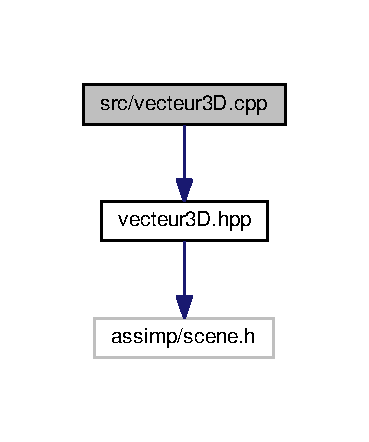
\includegraphics[width=177pt]{vecteur3_d_8cpp__incl}
\end{center}
\end{figure}


\subsection{Detailed Description}
Classe de vecteur en trois dimensions. 

\begin{DoxyAuthor}{Author}
Pierre Chevalier et Benoît Garçon 
\end{DoxyAuthor}
\begin{DoxyVersion}{Version}
1.\+0 
\end{DoxyVersion}
\begin{DoxyDate}{Date}
Octobre 2016 
\end{DoxyDate}

\hypertarget{vecteur3_d_8hpp}{\section{src/vecteur3\+D.hpp File Reference}
\label{vecteur3_d_8hpp}\index{src/vecteur3\+D.\+hpp@{src/vecteur3\+D.\+hpp}}
}


Classe de vecteur en trois dimensions.  


{\ttfamily \#include $<$assimp/scene.\+h$>$}\\*
Include dependency graph for vecteur3\+D.\+hpp\+:
\nopagebreak
\begin{figure}[H]
\begin{center}
\leavevmode
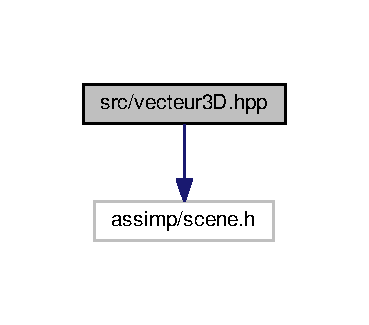
\includegraphics[width=177pt]{vecteur3_d_8hpp__incl}
\end{center}
\end{figure}
This graph shows which files directly or indirectly include this file\+:
\nopagebreak
\begin{figure}[H]
\begin{center}
\leavevmode
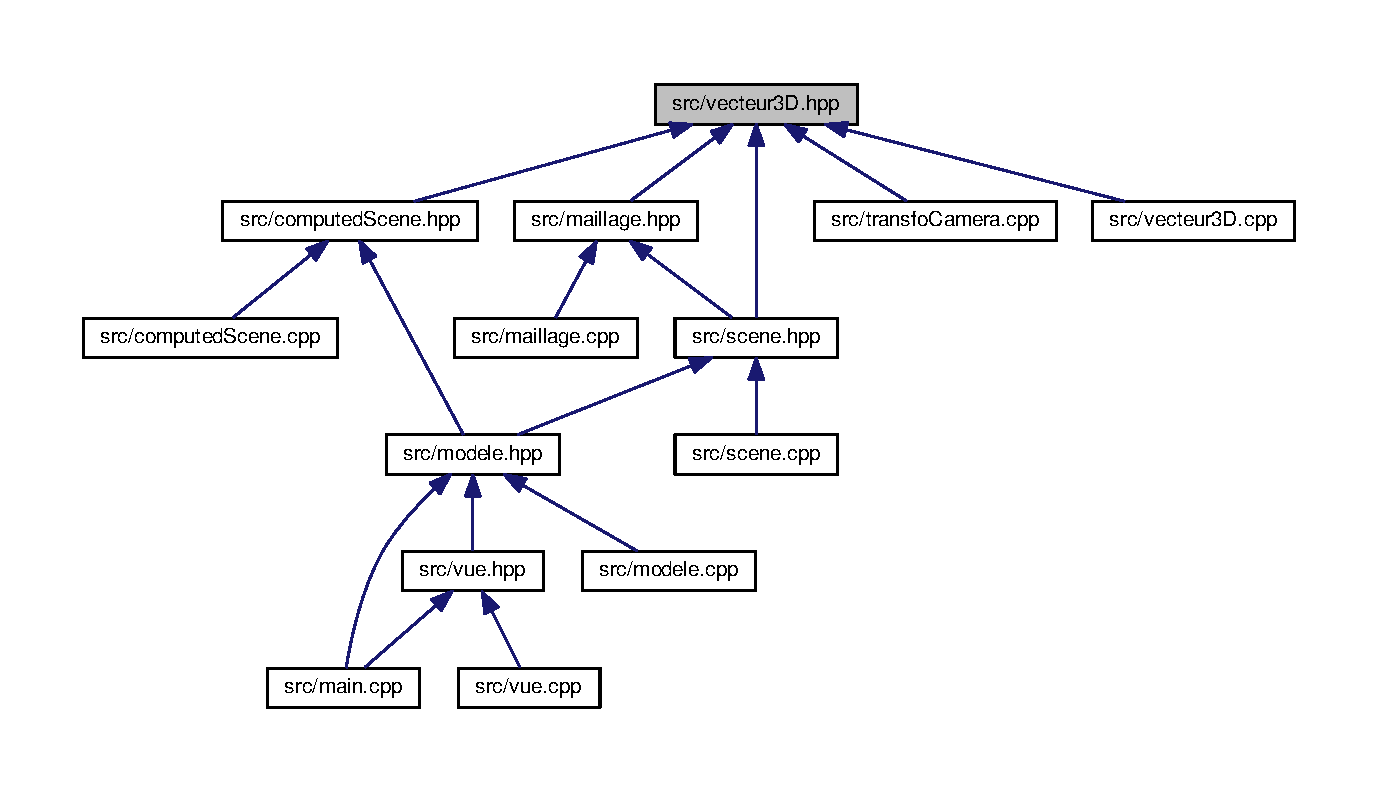
\includegraphics[width=350pt]{vecteur3_d_8hpp__dep__incl}
\end{center}
\end{figure}
\subsection*{Classes}
\begin{DoxyCompactItemize}
\item 
class \hyperlink{class_vecteur3_d}{Vecteur3\+D}
\begin{DoxyCompactList}\small\item\em Classe pour un vecteur 3\+D Cette classe encapsule les ai\+Vector3\+D. \end{DoxyCompactList}\end{DoxyCompactItemize}


\subsection{Detailed Description}
Classe de vecteur en trois dimensions. 

\begin{DoxyAuthor}{Author}
Pierre Chevalier et Benoît Garçon 
\end{DoxyAuthor}
\begin{DoxyVersion}{Version}
1.\+0 
\end{DoxyVersion}
\begin{DoxyDate}{Date}
Octobre 2016 
\end{DoxyDate}

\hypertarget{vue_8cpp}{}\section{src/vue.cpp File Reference}
\label{vue_8cpp}\index{src/vue.\+cpp@{src/vue.\+cpp}}


Classe de gestion de l\textquotesingle{}affichage.  


{\ttfamily \#include \char`\"{}vue.\+hpp\char`\"{}}\\*
{\ttfamily \#include $<$cstdio$>$}\\*
Include dependency graph for vue.\+cpp\+:
% FIG 0


\subsection{Detailed Description}
Classe de gestion de l\textquotesingle{}affichage. 

\begin{DoxyAuthor}{Author}
Pierre Chevalier et Benoît Garçon 
\end{DoxyAuthor}
\begin{DoxyVersion}{Version}
1.\+0 
\end{DoxyVersion}
\begin{DoxyDate}{Date}
Octobre 2016 
\end{DoxyDate}

\hypertarget{vue_8hpp}{\section{src/vue.hpp File Reference}
\label{vue_8hpp}\index{src/vue.\+hpp@{src/vue.\+hpp}}
}


Classe de gestion de l'affichage.  


{\ttfamily \#include $<$unistd.\+h$>$}\\*
{\ttfamily \#include $<$G\+L/glut.\+h$>$}\\*
{\ttfamily \#include \char`\"{}modele.\+hpp\char`\"{}}\\*
{\ttfamily \#include \char`\"{}frames.\+hpp\char`\"{}}\\*
{\ttfamily \#include \char`\"{}transfo\+Camera.\+hpp\char`\"{}}\\*
{\ttfamily \#include \char`\"{}look\+At\+Camera.\+hpp\char`\"{}}\\*
{\ttfamily \#include \char`\"{}./source\+Shading/light.\+hpp\char`\"{}}\\*
Include dependency graph for vue.\+hpp\+:
\nopagebreak
\begin{figure}[H]
\begin{center}
\leavevmode
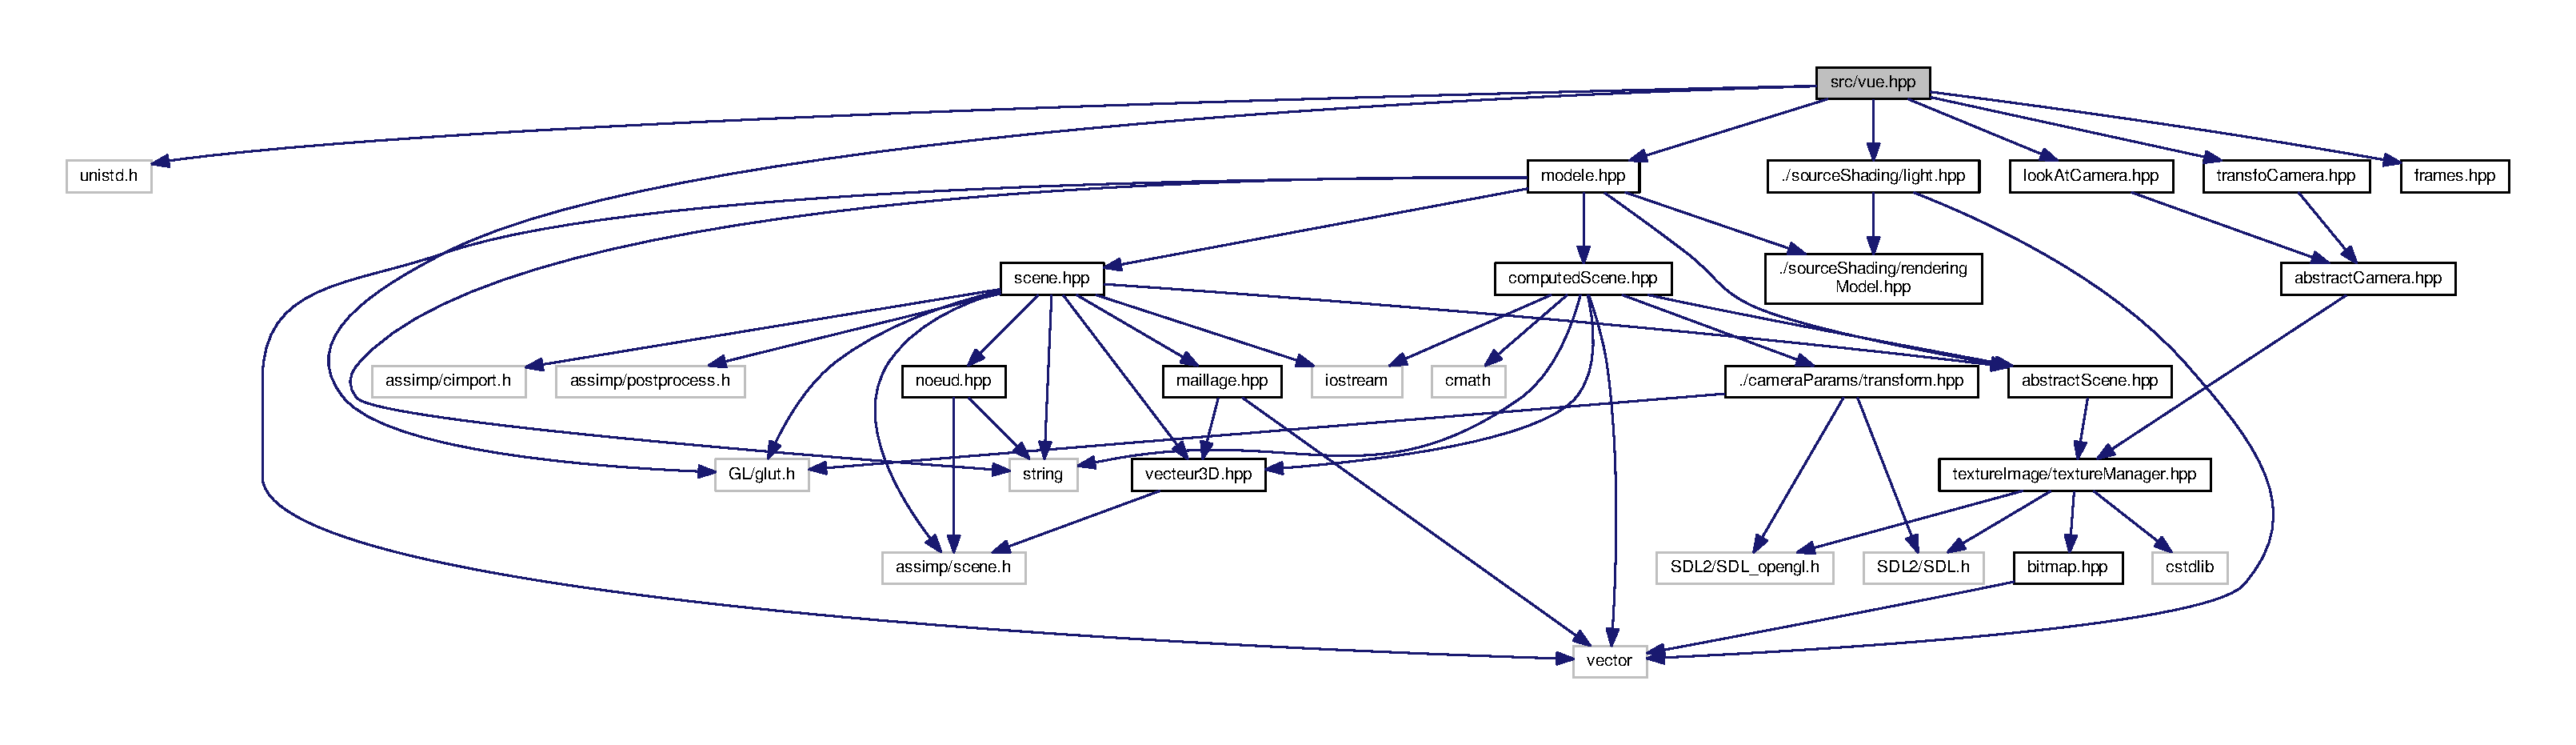
\includegraphics[width=350pt]{vue_8hpp__incl}
\end{center}
\end{figure}
This graph shows which files directly or indirectly include this file\+:
\nopagebreak
\begin{figure}[H]
\begin{center}
\leavevmode
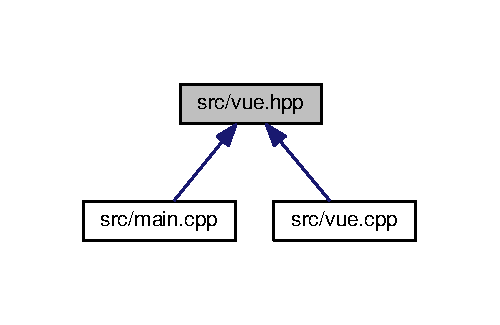
\includegraphics[width=240pt]{vue_8hpp__dep__incl}
\end{center}
\end{figure}
\subsection*{Classes}
\begin{DoxyCompactItemize}
\item 
class \hyperlink{class_display_manager}{Display\+Manager}
\begin{DoxyCompactList}\small\item\em Classe de gestion de l'affichage. Classe de gestion de l'affichage. \end{DoxyCompactList}\end{DoxyCompactItemize}


\subsection{Detailed Description}
Classe de gestion de l'affichage. 

\begin{DoxyAuthor}{Author}
Pierre Chevalier et Benoît Garçon 
\end{DoxyAuthor}
\begin{DoxyVersion}{Version}
1.\+0 
\end{DoxyVersion}
\begin{DoxyDate}{Date}
Octobre 2016 
\end{DoxyDate}

%--- End generated contents ---

% Index
\backmatter
\newpage
\phantomsection
\clearemptydoublepage
\addcontentsline{toc}{chapter}{Index}
\printindex

\end{document}
